\documentclass[11pt,a4paper,hidelinks]{article}

\setlength{\headheight}{26pt}

% Packages
\usepackage[left=25mm, right=25mm, top=35mm, bottom=25mm]{geometry} % defines whitespaces on the edges
\usepackage[bottom, hang]{footmisc}
\usepackage{hyperref}             % for \nameref and cite
\usepackage{footnotebackref}      % used for getting back from the footnote to the main text
\usepackage{enumitem}
\usepackage{graphicx}
\usepackage{fancyhdr}
\usepackage{lastpage}
\usepackage[export]{adjustbox}
\usepackage{float}
\usepackage[ngerman]{babel}
\usepackage[ngerman]{datetime}
\usepackage{apacite}
\usepackage[utf8]{inputenc}
\usepackage{listings}
\usepackage{xcolor}
\usepackage{pdfpages}
\usepackage{url}
\usepackage{outlines}
\usepackage{tocloft}
\usepackage[utf8]{inputenc}
\usepackage{amsmath}
\usepackage{mathtools}
\usepackage[acronym]{glossaries}
\usepackage{titlesec}             % for \titleformat
\usepackage{textcomp}             % for \degree sign
\usepackage{gensymb}              % for \degree sign
\usepackage{csvsimple}            % for using csv-files for tables
\usepackage{lscape}               % for landscape mode
\usepackage{parskip}              % inserts space after paragraph automatically
\usepackage{svg}                  % used to include svg with the help of inkscape which converts svg to pdf
\usepackage{wasysym}              % for \diameter symbol
\usepackage{xfrac}                % for \sfrac

\frenchspacing  % Use same space size between words and between sentences

% change section titles' font size
\titleformat*{\section}{\huge\bfseries}
\titleformat*{\subsection}{\LARGE\bfseries}
\titleformat*{\subsubsection}{\Large\bfseries}
\titleformat{\paragraph}[hang]{\large\bfseries}{\theparagraph}{1em}{}
\titleformat{\subparagraph}[hang]{\normalsize\bfseries}{\thesubparagraph}{1em}{}

\definecolor{codegreen}{rgb}{0,0.6,0}
\definecolor{codegray}{rgb}{0.5,0.5,0.5}
\definecolor{codepurple}{rgb}{0.58,0,0.82}
\definecolor{codeorange}{rgb}{1,0.5,0.15}
\definecolor{backcolour}{rgb}{0.9,0.9,0.9}

\lstdefinestyle{mystyle}{
    backgroundcolor=\color{backcolour},
    commentstyle=\color{codegreen},
    keywordstyle=\color{magenta},
    numberstyle=\tiny\color{codegray},
    stringstyle=\color{codepurple},
    basicstyle=\ttfamily\footnotesize,
    breakatwhitespace=false,
    breaklines=true,
    captionpos=b,
    keepspaces=true,
    numbers=left,
    numbersep=5pt,
    showspaces=false,
    showstringspaces=false,
    showtabs=false,
    tabsize=4
}
\lstset{style=mystyle}

\lstset{
    literate={~} {$\sim$}{1}
}

\lstset{%
    breaklines=true,
    breakatwhitespace=true,
}

\DeclarePairedDelimiter\abs{\lvert}{\rvert} % make scalable absolute stripes
\DeclarePairedDelimiter\parenth{(}{)} % make scalable parentheses

\let\phi\varphi{} % change style of \phi sign

\setlength{\parindent}{0mm} % disable paragraph indent

\newdateformat{mydate}{\THEDAY{. }\monthnamengerman[\THEMONTH] \THEYEAR}

\renewcommand{\listfigurename}{}
\renewcommand\contentsname{Inhaltsverzeichnis}
\renewcommand\lstlistingname{Code}

\makeglossaries{}

% Header/Footer Setting
\setlength\footnotemargin{15pt}
\pagestyle{fancy}
\fancyhf{}
\renewcommand{\footrulewidth}{0.4pt} % footer line
\rhead{\textbf{\vUniversity}\\\vModule}
\lhead{\textbf{\vTitle}\\
    Projektarbeit}
\lfoot{\vAuthorFirstName{} \vAuthorLastName}
\cfoot{\mydate\today}
\rfoot{S.~\thepage~/~\pageref{LastPage}}

% Redefine the plain page style, otherwise there is no header and footer for chapter pages
\fancypagestyle{plain}{%
    \fancyhf{}
    \renewcommand{\footrulewidth}{0.4pt} % footer line
    \rhead{\textbf{\vUniversity}\\\vModule}
    \lhead{\textbf{\vTitle}\\
        Projektarbeit}
    \lfoot{\vAuthorFirstName{} \vAuthorLastName}
    \cfoot{\mydate\today}
    \rfoot{S.~\thepage~/~\pageref{LastPage}}
}

\bibliographystyle{apacite}

% Settings for the equation list
\newcommand{\listequationsname}{}
\newlistof{myequations}{equ}{\listequationsname}
\renewcommand{\cftmyequationsaftersnum}{\hfill}
\renewcommand{\cftmyequationspresnum}{\hfill}
\setlength{\cftmyequationsnumwidth}{3.5em}
\newcommand{\myequations}[1]{%
\addcontentsline{equ}{myequations}{\protect\numberline{\theequation}#1}\par}

\newcommand{\mytable}[4]
{
    \centering
    \begin{tabular}{#1}\hline%
        #2 \\ \hline
        \csvreader[
            separator=semicolon,
            head to column names,
            late after line=\\,
        ]{#4}{}{#3}
        \hline
    \end{tabular}
}


% Variables
\newcommand{\vTitle}{DIY Optische ToF Distanzmessung}
\newcommand{\vModule}{CAS Sensorik und Sensor Signal Conditioning}
\newcommand{\vAuthorFirstName}{Matthias Schär,}
\newcommand{\vAuthorLastName}{Timon Burkard}
\newcommand{\vUniversity}{OST -- Ostschweizer Fachhochschule}
\newcommand{\vDegree}{CAS Sensorik und Sensor Signal Conditioning}
\newcommand{\vSemester}{HS24}
\newcommand{\vProfessor}{Prof. Guido Keel, Michael Lehmann}
\newcommand{\vCity}{Rapperswil}
\newcommand{\vAbstract}{
    Diese Projektarbeit behandelt die Entwicklung eines \acrfull{diy} Systems zur optischen \acrfull{tof} Distanzmessung.

    Um die Signallaufzeit präzise zu messen, wird ein \acrfull{tdc} eingesetzt. Zu Testzwecken wird ein zweiter
    \acrshort{tdc} verwendet, der rein elektrisch betrieben wird, um die Länge unterschiedlicher Kupferkabel zu
    bestimmen.

    Die Arbeit umfasst die Entwicklung der Hardware, einschließlich Lasertreiber, Photodetektor und
    Transimpedanzverstärker, sowie die Implementierung der Firmware zur Signalauswertung. Simulationen und Messungen
    wurden durchgeführt, um die Genauigkeit zu optimieren und Störfaktoren zu minimieren.

    Die elektrischen Messungen zeigen, dass der \acrshort{tdc} eine zeitliche Auflösung im Bereich einiger Dutzend
    Pikosekunden erreicht. Damit lassen sich Kabellängen auf wenige cm genau bestimmen.

    Die optischen Messungen zeigen, dass eine grobe Distanzmessung bis ca. 30~cm möglich ist, wenn ein Spiegel als
    Target eingesetzt wird. Um die Distanz zu einer Wand messen zu können, sind weiterführende Verbesserungen des
    Demonstrators notwendig.
}

% Acronyms
\newacronym{pcb}{PCB}{Printed Circuit Board}
\newacronym{tof}{ToF}{Time of Flight}
\newacronym{diy}{DIY}{Do It Yourself}
\newacronym{adc}{ADC}{Analog to Digital Converter}
\newacronym{tdc}{TDC}{Time to Digital Converter}
\newacronym{tia}{TIA}{Trans-Impedance Amplifier}
\newacronym{mcu}{MCU}{Microcontroller Unit}
\newacronym{cpu}{CPU}{Central Processing Unit}
\newacronym{hal}{HAL}{Hardware Abstraction Layer}
\newacronym{gpio}{GPIO}{General Purpose Input/Output}
\newacronym{uart}{UART}{Universal Asynchronous Receiver/Transmitter}
\newacronym{dso}{DSO}{Digital Storage Oscilloscope}
\newacronym{spi}{SPI}{Serial Peripheral Interface}
\newacronym{ic}{IC}{Integrated Circuit}
\newacronym{usb}{USB}{Universal Serial Bus}
\newacronym{hsi}{HSI}{High Speed Internal}
\newacronym{pll}{PLL}{Phase-Locked Loop}
\newacronym{ams}{AMS}{Analog/Mixed Signal}
\newacronym{fw}{FW}{Firmware}

\begin{document}

\title{\vspace{-40pt}\begin{huge}\textbf{\vTitle}\end{huge}\\
\ \\ \vModule}
\author{\\\\\textbf{\vAuthorFirstName{} \vAuthorLastName}\\
    \vUniversity{}\\
    \\\\}

\date{\mydate\today}
\maketitle\thispagestyle{empty}  % removes footer from first page

\vspace{35pt}

\begin{figure}[H]
    \centering
    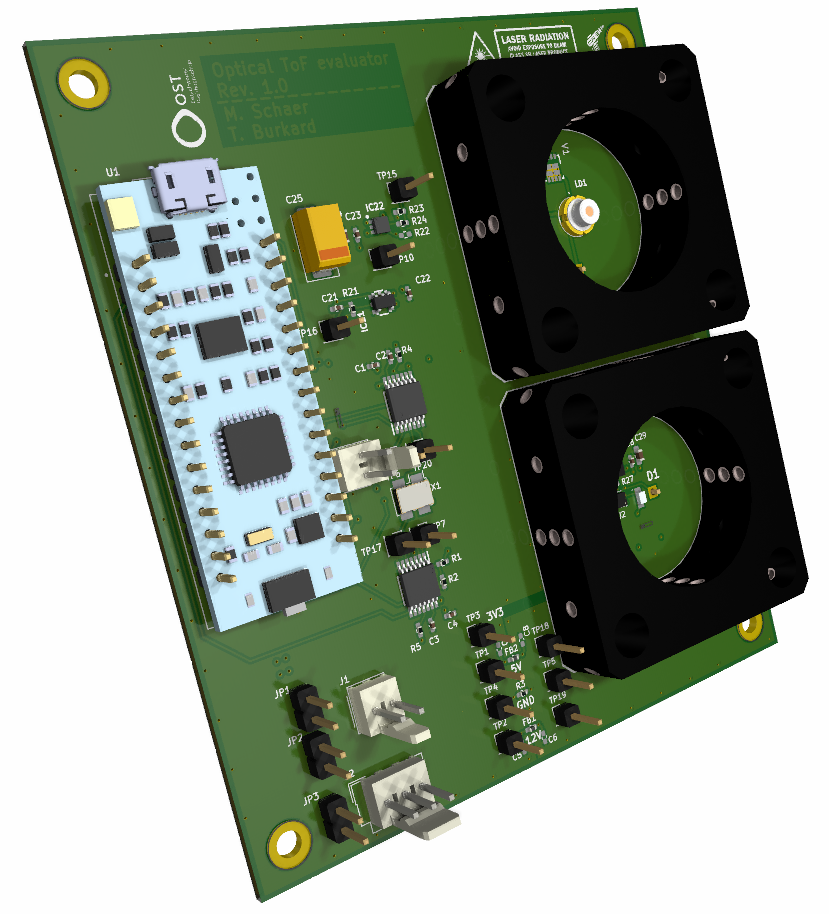
\includegraphics[width=0.6\textwidth]{graphics/cover_picture.png}
\end{figure}

\vspace{30pt}

\begin{figure}[H]
    \centering
    \begin{minipage}[b]{0.3\textwidth}
        \includesvg[width=\textwidth]{graphics/OST_Logo.svg}\label{fig:OST_Logo}
    \end{minipage}
\end{figure}

\pagebreak

\thispagestyle{empty}

\textbf{}
\vspace{5mm}

\begin{flushleft}
    \textbf{\large{\vModule{} an der \vUniversity{}}}
\end{flushleft}

\begin{flushleft}
    \begin{small}
        \begin{tabular}{@{}lll}
            \\
            \textbf{Titel}                 & & \textbf{\vTitle}\\
            \\
            \textbf{Diplomandin/Diplomand} & & \textbf{\vAuthorFirstName{} \vAuthorLastName}\\
            \\
            \textbf{Studiengang}           & & \textbf{\vDegree}\\
            \\
            \textbf{Semester}              & & \textbf{\vSemester}\\
            \\
            \textbf{Dozentin/Dozent}       & & \textbf{\vProfessor}\\
        \end{tabular}
    \end{small}
\end{flushleft}

\vspace{10mm}

% abstracts
\begin{flushleft}
    \begin{small}
        \textbf{Abstract} \\
        \vAbstract{}
        \vspace{15mm}
    \end{small}
\end{flushleft}

% copyright
\begin{flushleft}
    \begin{small}
        Ort, Datum\hspace{30mm}\vCity, \date{\mydate\today} \\
        \textbf{\textcopyright\hspace{1mm}\vAuthorFirstName{} \vAuthorLastName, \vUniversity{}}
    \end{small}
\end{flushleft}

\mbox{}
\vfill

\noindent\makebox[\linewidth]{\rule{\textwidth}{1pt}}
% copyright notice
\begin{flushleft}
    \begin{small}
        Alle Rechte vorbehalten. Die Arbeit oder Teile davon dürfen ohne schriftliche Genehmigung der Rechteinhaber weder in irgendeiner Form reproduziert noch elektronisch gespeichert, verarbeitet, vervielfältigt oder verbreitet werden.\\~\\
        Sofern die Arbeit auf der Website der Ostschweizer Fachhochschule online veröffentlicht wird, können abweichende Nutzungsbedingungen unter Creative-Commons-Lizenzen gelten. Massgebend ist in diesem Fall die auf der Website angezeigte Creative-Commons-Lizenz.
    \end{small}
\end{flushleft}

\pagebreak

\section*{Inhaltsverzeichnis}
\vspace{-25pt}
\renewcommand*\contentsname{}
\tableofcontents

\pagebreak

\section*{Abkürzungsverzeichnis}
\vspace{-25pt}
\printglossary[type=\acronymtype,title={}]

\pagebreak

\section*{Abbildungsverzeichnis}
\vspace{-25pt}
\renewcommand{\listfigurename}{}
\listoffigures

\pagebreak

\section*{Formelverzeichnis}
\vspace{-25pt}
\listofmyequations{}

\pagebreak

\section*{Tabellenverzeichnis}
\vspace{-25pt}
\renewcommand{\listtablename}{}
\listoftables

\pagebreak

\section*{Codeverzeichnis}
\vspace{-33pt}
\renewcommand{\lstlistlistingname}{}
\lstlistoflistings{}

\pagebreak


%%%%%%%%%%%%%%%%%%%%%% CONTENT START %%%%%%%%%%%%%%%%%%%%%%

\section{Einleitung}\label{sec:introduction}
Bei dieser Projektarbeit geht es darum ein \acrfull{diy} optisches \acrfull{tof} Distanzmesssystem aufzubauen. Dazu soll
ein \acrfull{tdc} verwendet werden.

\dots

\pagebreak

\section{Theorie}\label{sec:theory}
\subsection{Time of Flight}

Bei \acrshort{tof} handelt es sich um \dots

\pagebreak

\subsection{Photostrom}

Zur Berechnung des theoretisch zu erwartenden Photostrom wird von einer Distanz zur Wand von $10~m$ ausgegangen.

Der Laserstrahl gehe idealisiert mit $0\degree$ zur Wand und werde dort uniform Halbkugel-förmig gestreut. In der
Realität wird der Laser nicht mit $0\degree$ zur Wand gehen und die Streuung wird sich nicht uniform verteilen, sondern
in der Mitte stärker konzentriert sein.

Die Berechnung der empfangenen Strahlungsleistung, der Strahlungsintensität, dem Raumwinkel und dem Photostrom sind in
Formel~\ref{eq:pin}, \ref{eq:ie}, \ref{eq:omega} bzw. \ref{eq:iph} gezeigt.

\begin{equation}\label{eq:pin}
    P_{in} = E_e \cdot A = \frac{I_e}{r^2} \cdot A
\end{equation}
\myequations{Eintreffende Lichtleistung}

\begin{equation}\label{eq:ie}
    I_e = \frac{P_{out}}{\Omega}
\end{equation}
\myequations{Strahlungsintensität}

\begin{equation}\label{eq:omega}
    \Omega = \frac{4\cdot \pi \cdot 0.5}{d}
\end{equation}
\myequations{Raumwinkel}

\begin{equation}\label{eq:iph}
    I_{ph} = S \cdot P_{in}
\end{equation}
\myequations{Photostrom}

\subsubsection{Berechnung mit RLD94PZJ5 und BPV23NF}

Ersten Berechnungen wurden mit der Laserdiode RLD94PZJ5 \cite{rohm2020rld94pzj5_datasheet} und der Photodiode BPV23NF
\cite{vishay2024bpv23nf_datasheet} durchgeführt.

Die relevanten Werte aus den Datenblättern sind in Formel~\ref{eq:rld94pzj5_num} und \ref{eq:rbpv23nf_num} aufgelistet.

\begin{equation}\label{eq:rld94pzj5_num}
    P_{out} = 285~mW
\end{equation}
\myequations{Werte des RLD94PZJ5}

\begin{equation}\label{eq:rbpv23nf_num}
    \begin{split}
        A &= 4.4~mm^2\\
        S &= 0.6~\frac{A}{W}
    \end{split}
\end{equation}
\myequations{Werte des BPV23NF}

Diese Werte eingesetzt in Formel~\ref{eq:ie}, \ref{eq:pin} und \ref{eq:iph} ergibt die Resultate in
Formel~\ref{eq:rld94pzj5_rbpv23nf_num}.

\begin{equation}\label{eq:rld94pzj5_rbpv23nf_num}
    \begin{split}
        I_e    &= \frac{P_{out}}{\Omega} = \frac{285~mW}{\frac{4\cdot \pi \cdot 0.5}{d}} = \frac{285~mW}{\frac{4\cdot \pi \cdot 0.5}{10~m}} = 45~\frac{mW}{sr}\\
        P_{in} &= \frac{I_e}{r^2} \cdot A = 45~\frac{mW}{sr} \cdot 4.4~mm^2 = 2~nW\\
        I_{ph} &= S \cdot P_{in} = 0.6~\frac{A}{W} \cdot 2~nW = 1.2~nA
    \end{split}
\end{equation}
\myequations{Nummerische Resultate mit RLD94PZJ5 und BPV23NF}

\subsubsection{Berechnung mit RLD65NZX1 and NJL6401R-3}

Die Laserdiode RLD94PZJ5 hat im Bezug auf diese Projektarbeit zwei Nachteile: Sehr hohe Leistung, welche für das
menschliche Auge gefährlich werden kann und ein Wellenlängenbereich, der für das menschliche Auge nicht sichtbar ist.

Aus diesen Gründen wurde eine zweite Laserdiode evaluiert: RLD65NZX1 \cite{rohm2019rld65nzx1_datasheet}. Gepaart wird
sie mit der Photodiode NJL6401R-3 \cite{jrc2014njl6401r3_datasheet}. Die folgenden Berechnungen wurden basierend auf
diesen beiden Komponenten durchgeführt.

Die relevanten Werte aus den Datenblättern sind in Formel~\ref{eq:rld65nzx1_num} und \ref{eq:njl6401r3_num} aufgelistet.

\begin{equation}\label{eq:rld65nzx1_num}
    P_{out} = 10~mW
\end{equation}
\myequations{Werte des RLD65NZX1}

\begin{equation}\label{eq:njl6401r3_num}
    \begin{split}
        A &= 0.7~mm \cdot 0.7~mm = 0.49~mm^2\\
        S &= 0.42~\frac{A}{W}
    \end{split}
\end{equation}
\myequations{Werte des NJL6401R-3}

Diese Werte eingesetzt in Formel~\ref{eq:ie}, \ref{eq:pin} und \ref{eq:iph} ergibt die Resultate in
Formel~\ref{eq:rld65nzx1_njl6401r3_num}.

\begin{equation}\label{eq:rld65nzx1_njl6401r3_num}
    \begin{split}
        I_e    &= \frac{P_{out}}{\Omega} = \frac{10~mW}{\frac{4\cdot \pi \cdot 0.5}{d}} = \frac{10~mW}{\frac{4\cdot \pi \cdot 0.5}{10~m}} = 1.6~\frac{mW}{sr}\\
        P_{in} &= \frac{I_e}{r^2} \cdot A = 45~\frac{mW}{sr} \cdot 0.49~mm^2 = 8~pW\\
        I_{ph} &= S \cdot P_{in} = 0.42~\frac{A}{W} \cdot 8~pW = 3.3~pA
    \end{split}
\end{equation}
\myequations{Nummerische Resultate mit RLD65NZX1 and NJL6401R-3}

\subsubsection{Berechnung mit Empfangs-Linse}

Auf Vorschlag der Dozenten wurden verschiedene Optiken aus einem Baukasten-System von QIOPTIQ ausprobiert.
Besonders vielversprechend erschien hierbei eine Linse mit einem Durchmesser von 17~mm bei einer Brennweite von
40~mm. Die Linse ist in Abbildung~\ref{fig:lens} dargestellt.

\begin{figure}[H]
    \centering
    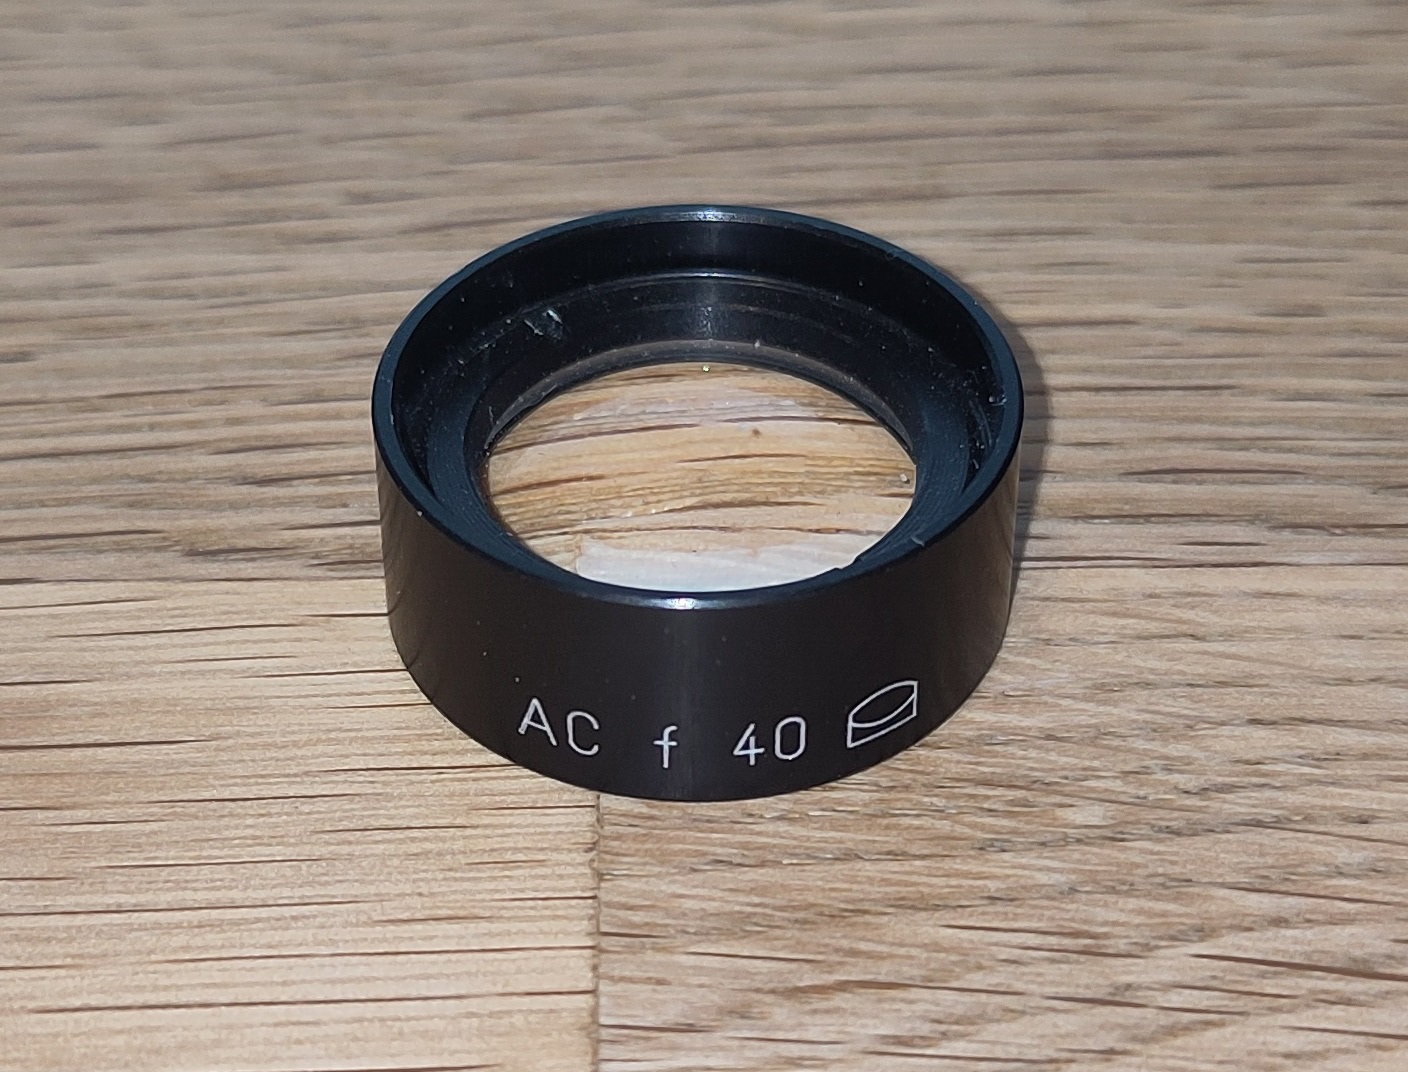
\includegraphics[width=0.5\textwidth]{graphics/photo_lens.jpg}
    \caption{Linse von QIOPTIQ}\label{fig:lens}
\end{figure}

Eine Solche Linse vergrössert die effektive Fläche, auf welcher der Lichtstrom empfangen werden kann, was
eine höhere Empfangsleistung, sprich einen höheren Lichtstrom zur Folge hat.

Im Idealfall kann diese Optik die Fläche um etwa folgenden Faktor vergrössern:

\begin{equation}\label{eq:njl6401r3_lens}
    A' = \frac{A_{L}}{A_{PD}} = \frac{(\frac{17~mm}{2})^2 \cdot \pi}{0.49~mm^2} = 463.2
\end{equation}
\myequations{Vergrösserung der Empfangsfläche durch Linse}

\textcolor{red}{TODO: Wollen wir hier noch eine bessere Annäherung für den Laser machen?}

\pagebreak

\subsection{Transimpedanzverstärker}

Bei einem \acrfull{tia} handelt es sich um \dots

\pagebreak

\section{Konzept}\label{sec:concept}
Die folgenden Unterkapitel klären über die Entwicklungsarbeiten auf, welche für das Umsetzen des \acrshort{tof}-Demonstrators
nötig sind. Hierbei wird vor allem darauf eingegangen, wie die Elektronik aufgebaut sein kann. Zudem werden weitere
Herausforderungen eines solchen Systems und die mögliche Bewältigung ebendieser aufgezeigt.

\subsection{Signalkette}

Nachfolgend sind einige Erklärungen dazu zu finden, wie die \acrshort{tof}-Messung realisiert wird.

Ein Blockdiagramm des Gesamtprojektes, bestehend aus dem elektrischen und dem optischen Teil, ist in
Abbildung~\ref{fig:blockdiagram} dargestellt.

\begin{figure}[H]
    \centering
    \includegraphics[width=0.8\textwidth]{diagrams/blockdiagram.pdf}
    \caption{Blockdiagramm}\label{fig:blockdiagram}
\end{figure}

Eine detailliertere Skizze der optischen Signalkette ist in der Abbildung~\ref{fig:konzept_signalpfad} ersichtlich.

\begin{figure}[H]
    \centering
    \includegraphics[width=\textwidth]{diagrams/konzept_signalpfad.pdf}
    \caption{Konzeptioneller Signalpfad}\label{fig:konzept_signalpfad}
\end{figure}

Eine \acrshort{mcu} kümmert sich um das Starten und Auswerten der Messresultate. Das Generieren eines Startsignals hat
zur Folge, dass über einen Laser-Treiber eine Laser-Diode mit einem Puls angesteuert wird. Dieser Puls, nach der Laser-Diode
in Form eines Lichtpulses, wird dann von einem Target reflektiert, welches in einer variablen Distanz zur Elektronik steht.

Der reflektierte Lichtpuls wird über eine Optik fokussiert und anschliessend von einer Photo-Diode in einen
Lichtstrom umgewandelt. Dieser Lichtstrom wird von einem Transimpedanzverstärker in eine Spannung umgewandelt. Bevor die
\acrshort{mcu} diese Spannung auswerten kann, muss diese erst digitalisiert werden. Dies passiert unter Verwendung eines Komparators.
Dieser kann als 1~bit \acrshort{adc} verstanden werden, da bloss eine Unterscheidung der beiden Zustände \dq Licht\dq\ und
\dq kein Licht\dq\ notwendig ist. Es ergibt sich also ein Empfangspuls.

Wird nun die Zeit gemessen zwischen Startsignal und empfangenem Puls, ist es möglich einen Rückschluss zu ziehen über die variable Strecke
zwischen Elektronik und Target. Die Zeitmessung unterliegt höchsten Anforderungen. Als Versinnbildlichung: Innert einer Nanosekunde
kann Licht eine Distanz von 30~cm zurücklegen. Wie eine solche Zeitmessung realisiert werden kann, erklärt das nächste Unterkapitel.

\subsection{Zeitmessung}

Damit ein direct \acrshort{tof}-Signal ausgewertet werden kann, benötigt es eine hochaufgelöste
Zeitmessung. Die Firma Texas Instruments bietet dafür mit dem TDC7200 eine gute Lösung
an. Laut Datenblatt \cite{ti2016tdc7200_datasheet} kann dieser bis zu 55~ps auflösen, mit einer
Standardabweichung von 35~ps. Setzt man nun die Lichtgeschwindigkeit sowie diese minimale
zeitliche Auflösung in eine Bewegungsgleichung ein, sollte der Baustein gemäss der Formel~\ref{eq:tdc_max_resolution}
folgende räumliche Auflösung erreichen:

\begin{equation}\label{eq:tdc_max_resolution}
        s_{min} = c \cdot t = 299.8 \cdot 10^6~\frac{m}{s} \cdot 55~ps = 16.5~mm
\end{equation}
\myequations{Maximale räumliche Auflösung des TDC7200}

Prinzipiell soll die \acrshort{tof}-Funktionalität in zwei Schritten in Betrieb genommen werden.
In einem ersten Teil soll es rein darum gehen, den TDC7200 \acrshort{ic} genauer
kennenzulernen.

Bemerkung: In der Realität wird eine solche Auflösung nicht erreichbar sein. Die Herausforderungen
bestehen beispielsweise darin, dass in der gesamten Signalkette diverse Verzögerungen vorhanden sind.
So spielen zum Beispiel das Einschalten der Laser-Diode, die Bandbreite des Verstärkers sowie
die Schaltzeit des Komparators eine grosse Rolle. Auch der Jitter der \acrshort{mcu} beim Ein- und Ausschalten
ihrer Ausgänge wird bei der minimalen Auflösung ins Gewicht fallen. Im Kapitel~\ref{sec:electrical_measurements}
wird mittels verschiedener Messungen dargestellt, wie nah an die vom TDC7200 vorgegebene Grenze herangekommen wird.

\subsection{Vorgehensweise}\label{sec:approach}

Wie bereits erläutert ist davon auszugehen, dass der gesamte Signalpfad eine Ungenauigkeit in die Messung einbringt,
welche weit ausserhalb derjenigen des TDC7200 liegt. Es bietet sich also an, dass diese im Vorfeld untersucht wird.
Dazu wird ein zweiter TDC7200 auf der Elektronik eingesetzt, welcher zur Messung eines rein elektrischen Signals
zuständig ist.

\begin{figure}[H]
    \centering
    \includegraphics[width=\textwidth]{diagrams/konzept_tdc_electrical.pdf}
    \caption{Konzept Betrieb \acrshort{tdc} rein elektrisch}\label{fig:konzept_tdc_electrical}
\end{figure}

In Abbildung~\ref{fig:konzept_tdc_electrical} sei skizziert, wie eine solche Schaltung aussehen könnte. Die gewellte,
rot markierte Linie versinnbildlicht dabei einen variablen Messpfad. Über einen Stecker können hier unterschiedlich lange
Kabel angeschlossen werden. Somit ist es möglich, die Messgenauigkeit des TDC7200 rein elektrisch nachzuweisen.

Folgende Punkte können mit einer solchen Erweiterung überprüft werden:

\begin{itemize}
    \item Messung Jitter der Ausgänge der verwendeten \acrshort{mcu}
    \item Konfiguration und Inbetriebnahme TDC7200 (z.B. verschiedene Messmodi)
    \item Auswertung der Resultate des TDC7200
\end{itemize}

\pagebreak

\section{Simulationen}\label{sec:simulations}
In diesem Kapitel werden die durchgeführten Simulationen dokumentiert.

Zur Simulation wird das Tool \dq Xpedition AMS\dq\ von Siemens verwendet. Wie der Name sagt, unterstützt dieses Tool
\acrfull{ams} Analyse. \cite{siemens2025xpeditionams}

\subsection{Laser Treiber}

In Abbildung~\ref{fig:simulation_laser_driver_schematic} ist das Schema für die Simulation des Laser-Treibers
dargestellt. Dies entspricht der Schaltung aus Kapitel~\ref{sec:schematic_laser_driver}.

\begin{figure}[H]
    \centering
    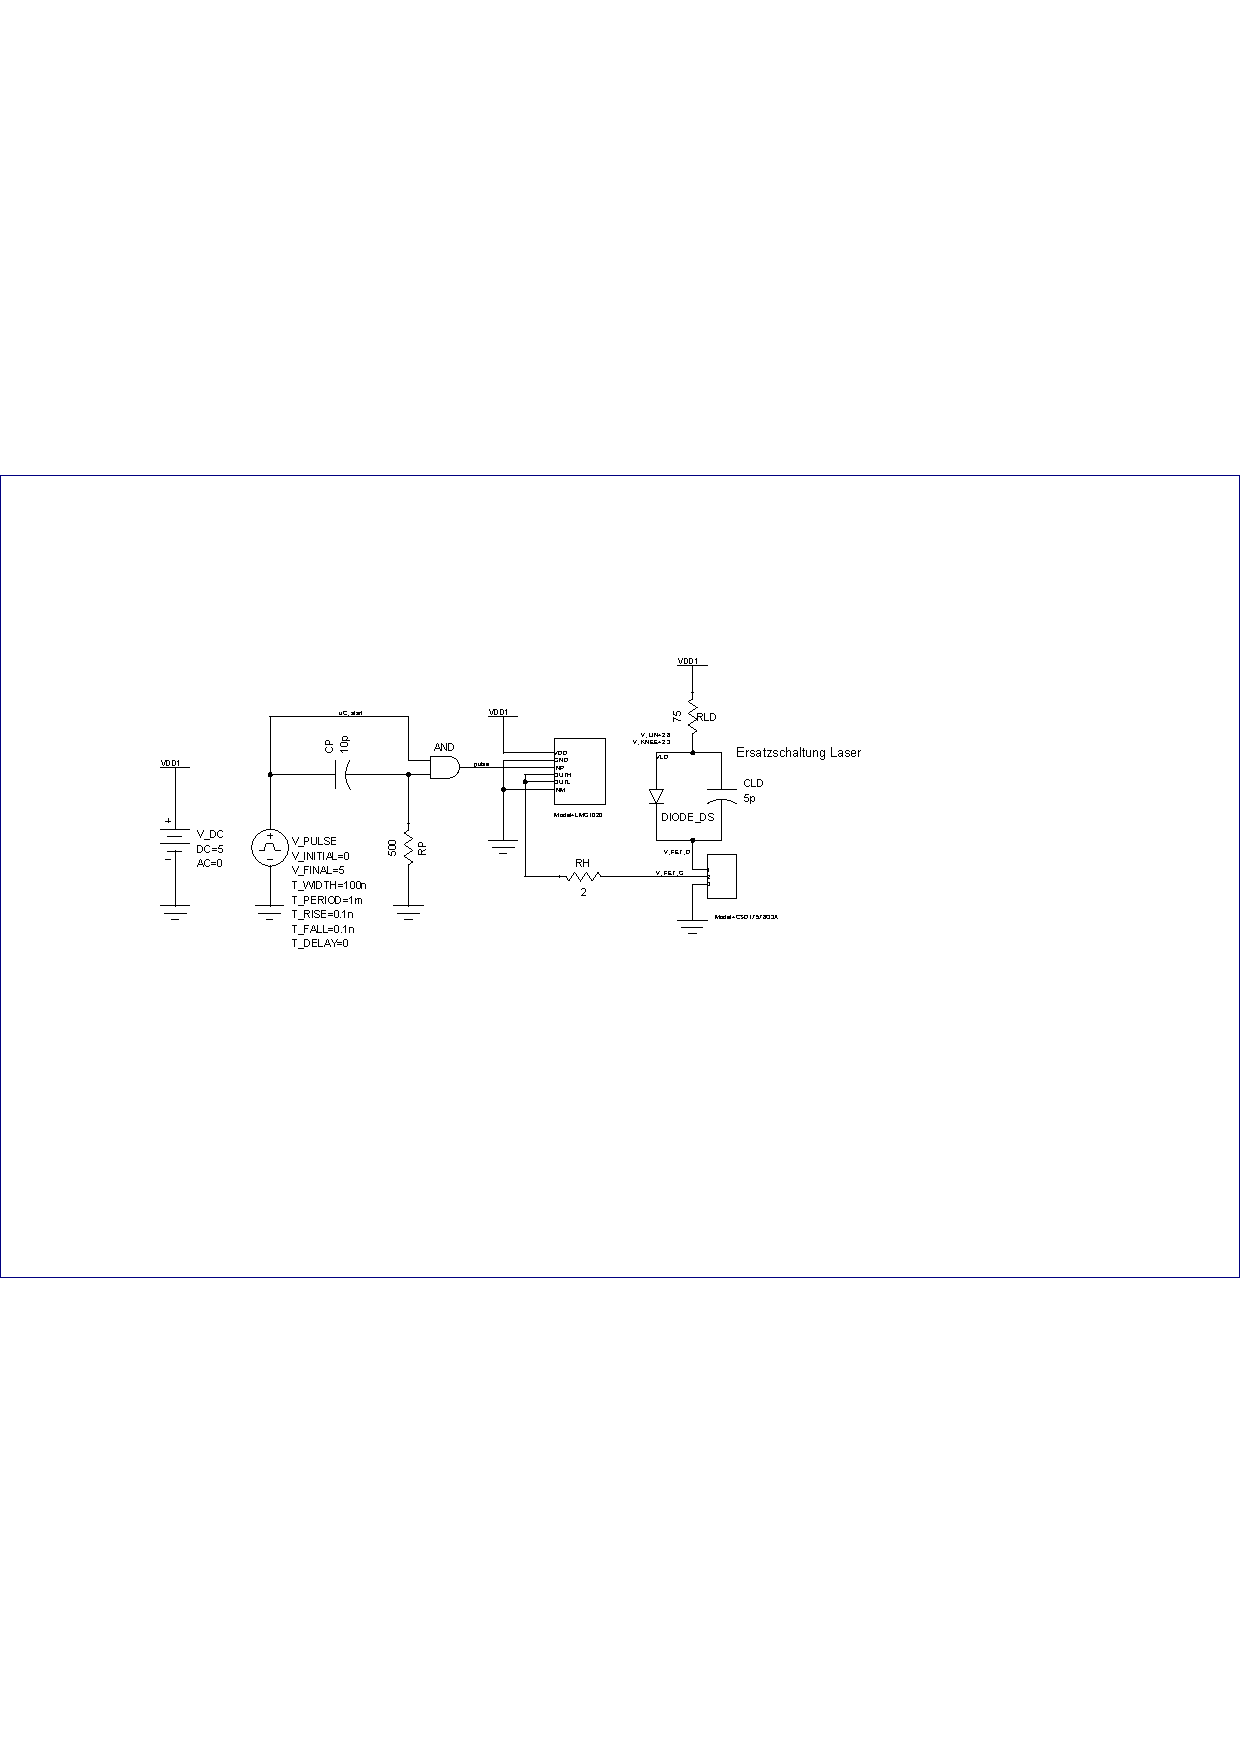
\includegraphics[trim=70 380 180 310, clip, width=0.9\textwidth]{attachments/simulation_laser_driver_schematic.pdf}
    \caption{Simulation Laser-Treiber - Schema}\label{fig:simulation_laser_driver_schematic}
\end{figure}

Das SPICE-Modell des Gate-Treibers LMG1025-Q1 ist dasselbe wie für LMG1020 und wurde von der Website von TI
heruntergeladen \cite{ti2024lmg1025q1}.

Das SPICE-Modell des NexFET CSD17578Q3A wurde ebenfalls von der Website von TI heruntergeladen
\cite{ti2024csd17578q3a}.

Für die Laser-Diode RLD65NZX1 konnte kein SPICE-Modell gefunden werden, es wurde deshalb eine Ersatzschaltung aus Diode
und paralleler, parasitärer Kapazität eingefügt.

Das Resultat der Simulation ist in Abbildung~\ref{fig:simulation_laser_driver_plot} dargestellt.

\begin{figure}[H]
    \centering
    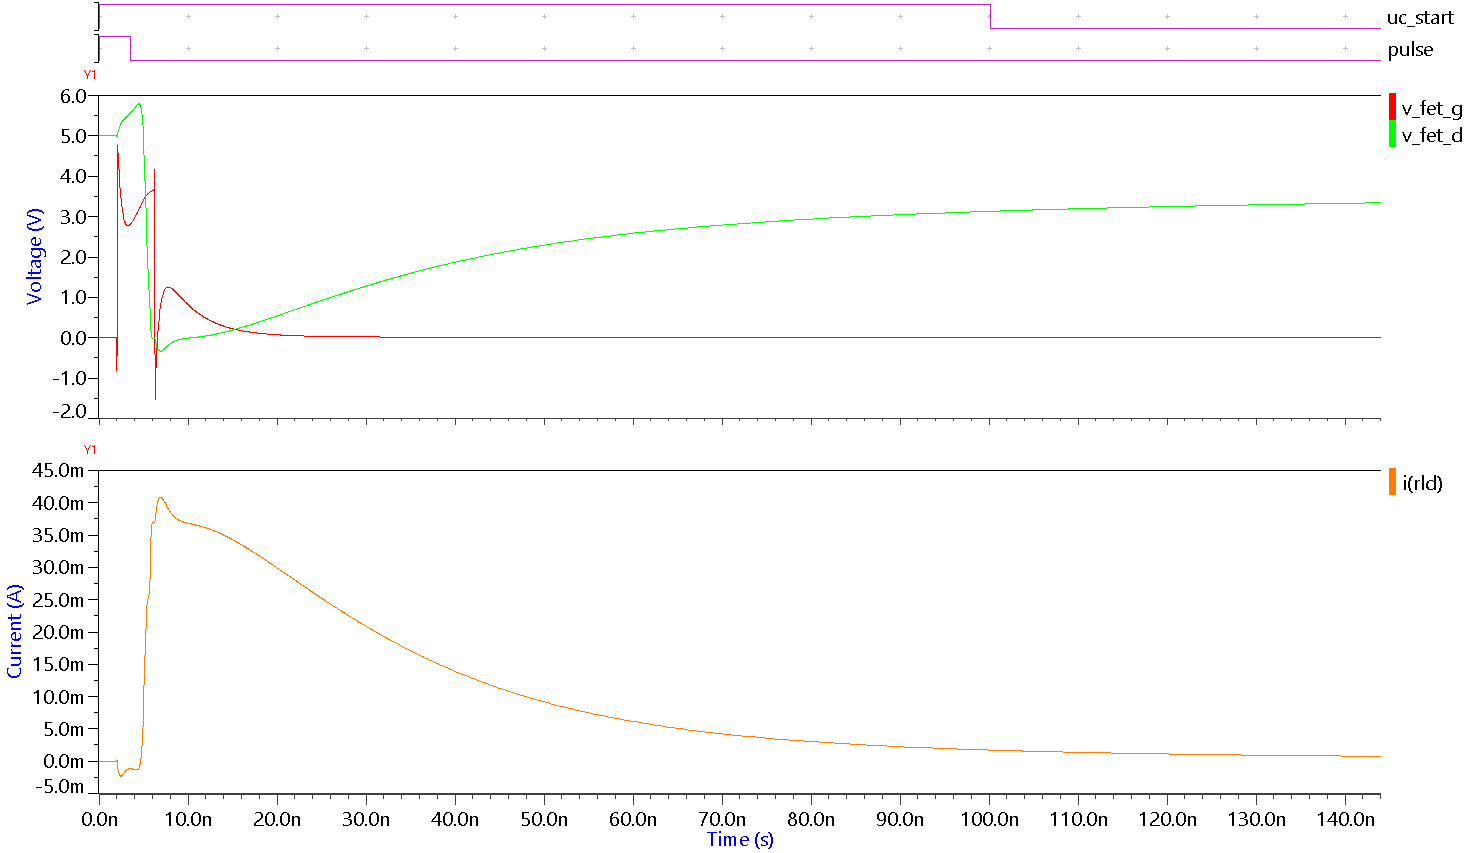
\includegraphics[width=\textwidth]{graphics/simulation_laser_driver_plot.png}
    \caption{Simulation Laser-Treiber - Plot}\label{fig:simulation_laser_driver_plot}
\end{figure}

Es ist zu erkennen, dass der Laser sehr schnell einschalten kann (2 \dots 3~ns). Das Ausschalten dauert etwas länger
(ca. 100~ns). Da die \acrshort{tof} bis zur ersten Flanke gemessen wird, ist eine längere Ausschaltzeit für diese
Anwendung kein Problem.

\subsection{Transimpedanzverstärker}

In Abbildung~\ref{fig:simulation_tia_schematic} ist das Schema für die Simulation des Transimpedanzverstärkers
dargestellt. Dies entspricht der Schaltung aus Kapitel~\ref{sec:schematic_photo_receiver}, ohne den Komparator.

\begin{figure}[H]
    \centering
    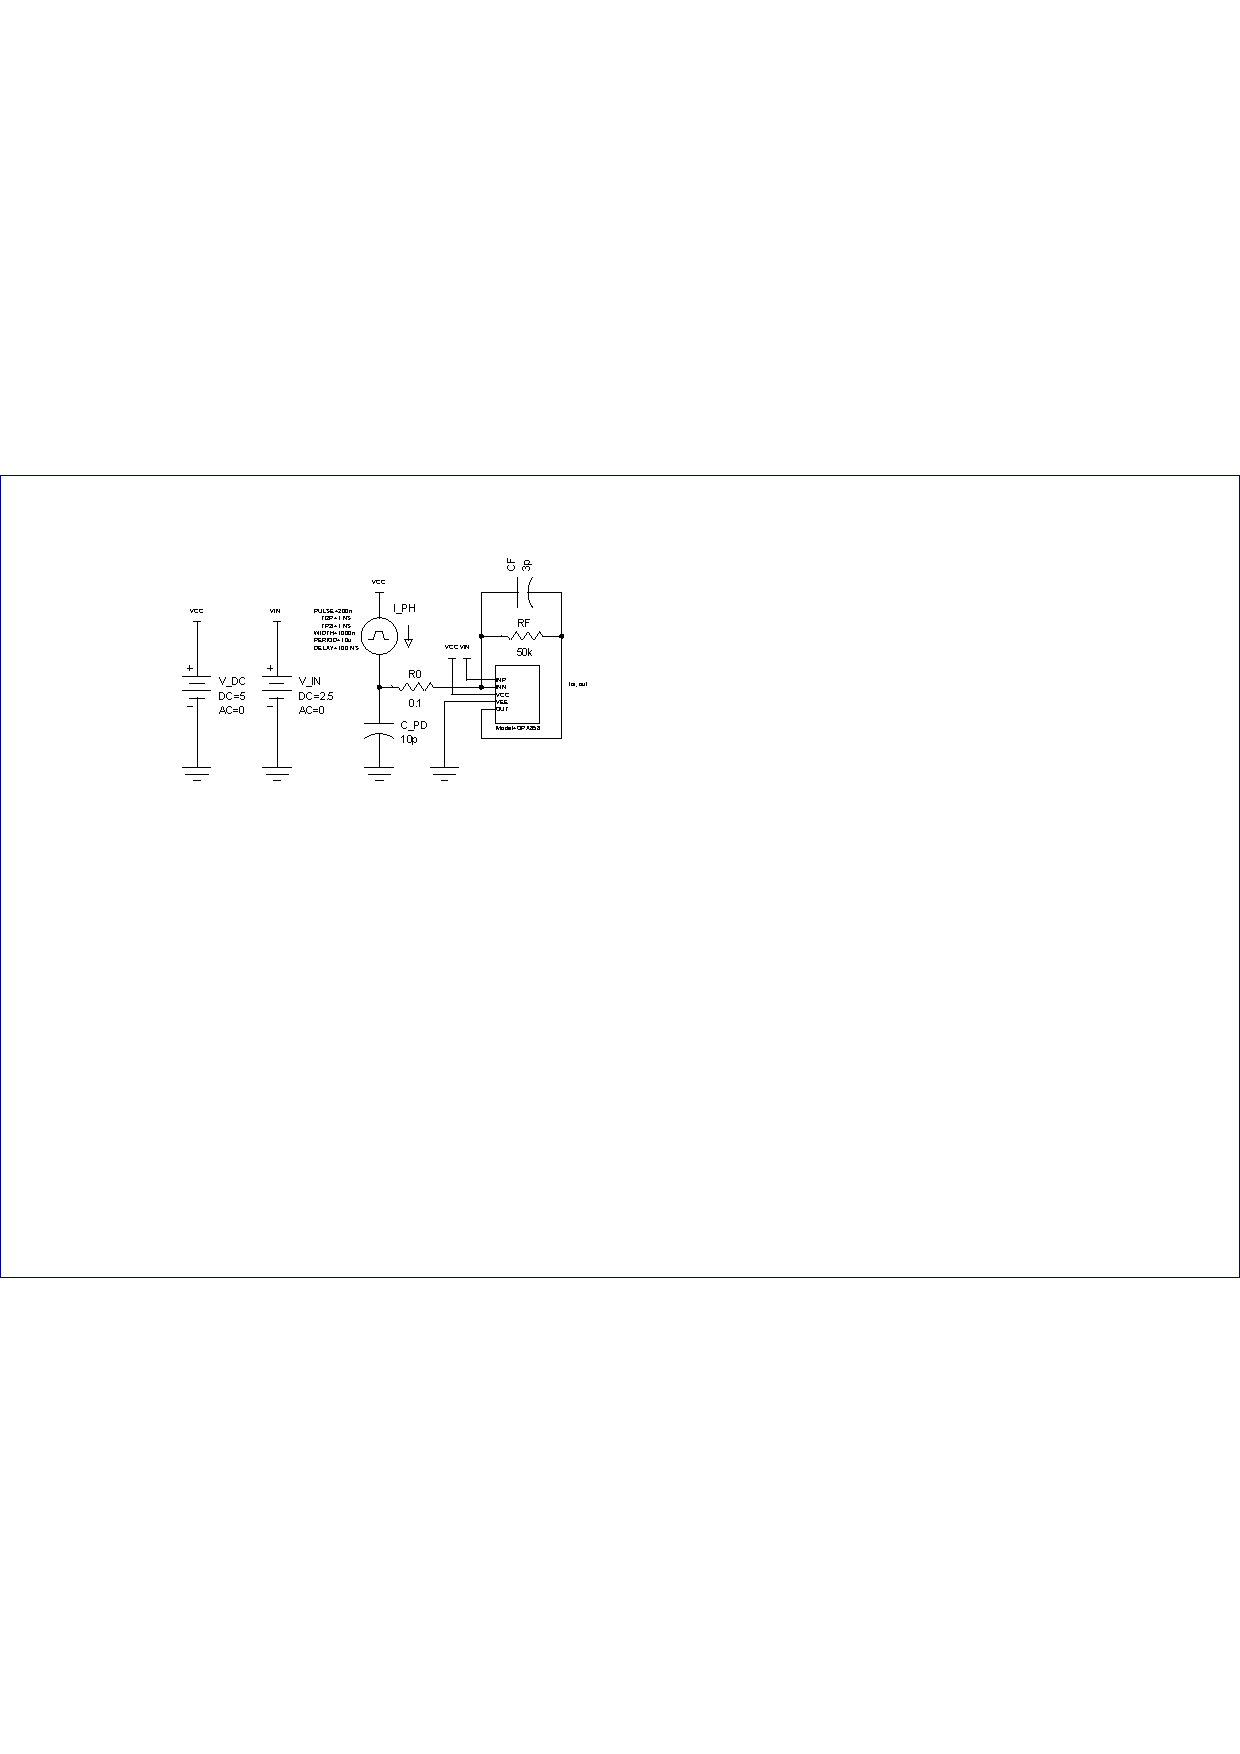
\includegraphics[trim=80 465 310 265, clip, width=0.7\textwidth]{attachments/simulation_tia_schematic.pdf}
    \caption{Simulation \acrshort{tia} - Schema}\label{fig:simulation_tia_schematic}
\end{figure}

Das SPICE-Modell des Operationsverstärkers OPA858 wurde von der Website von TI heruntergeladen \cite{ti2024opa858}.

Für die Photo-Diode NJL6401R konnte kein SPICE-Modell gefunden werden, es wurde deshalb eine Ersatzschaltung aus
Strompuls-Quelle und paralleler, parasitärer Kapazität eingefügt.

Das Resultat der Simulation ist in Abbildung~\ref{fig:simulation_tia_plot} dargestellt.

\begin{figure}[H]
    \centering
    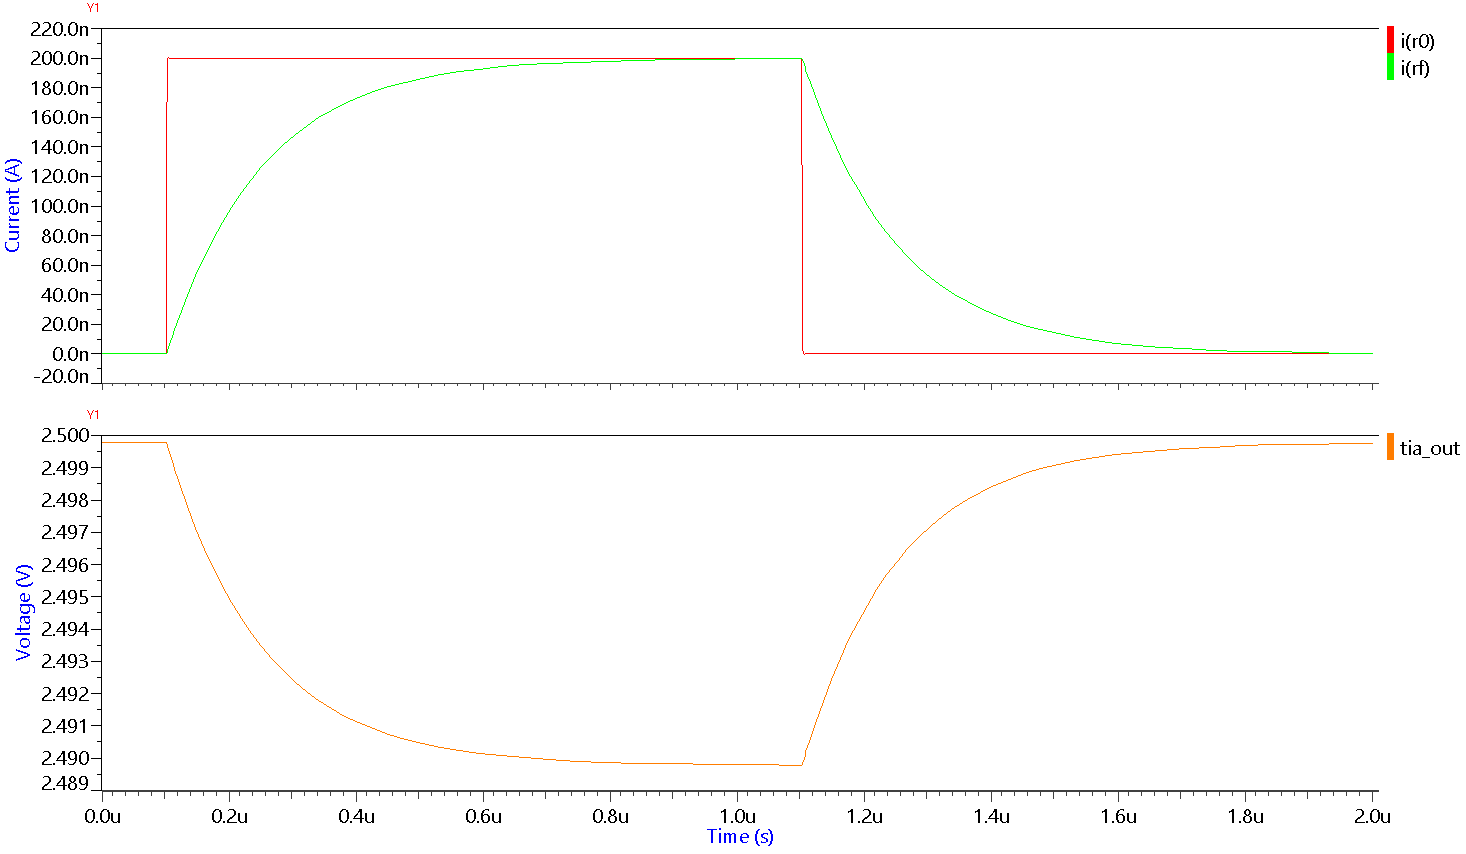
\includegraphics[width=\textwidth]{graphics/simulation_tia_plot.png}
    \caption{Simulation \acrshort{tia} - Plot}\label{fig:simulation_tia_plot}
\end{figure}

Es ist zu erkennen, dass die Zeitkonstante des Stroms durch den Feedback-Widerstand \lstinline|RF| gemäss
Formel~\ref{eq:tia_tau} bestimmt werden kann.

\begin{equation}\label{eq:tia_tau}
    \tau = R_F \cdot C_F = 50~k\Omega \cdot 3~pF = 150~ns
\end{equation}
\myequations{\acrshort{tia} Zeitkonstante}

Beliebig klein kann der Feedback-Kondensator \lstinline|CF| jedoch nicht gewählt werden, da die Schaltung sonst schwingt.

In Abbildung~\ref{fig:simulation_tia_plot_wo_cf} ist das Simulations-Resultat ohne den Feedback-Kondensator
\lstinline|CF| dargestellt.

\begin{figure}[H]
    \centering
    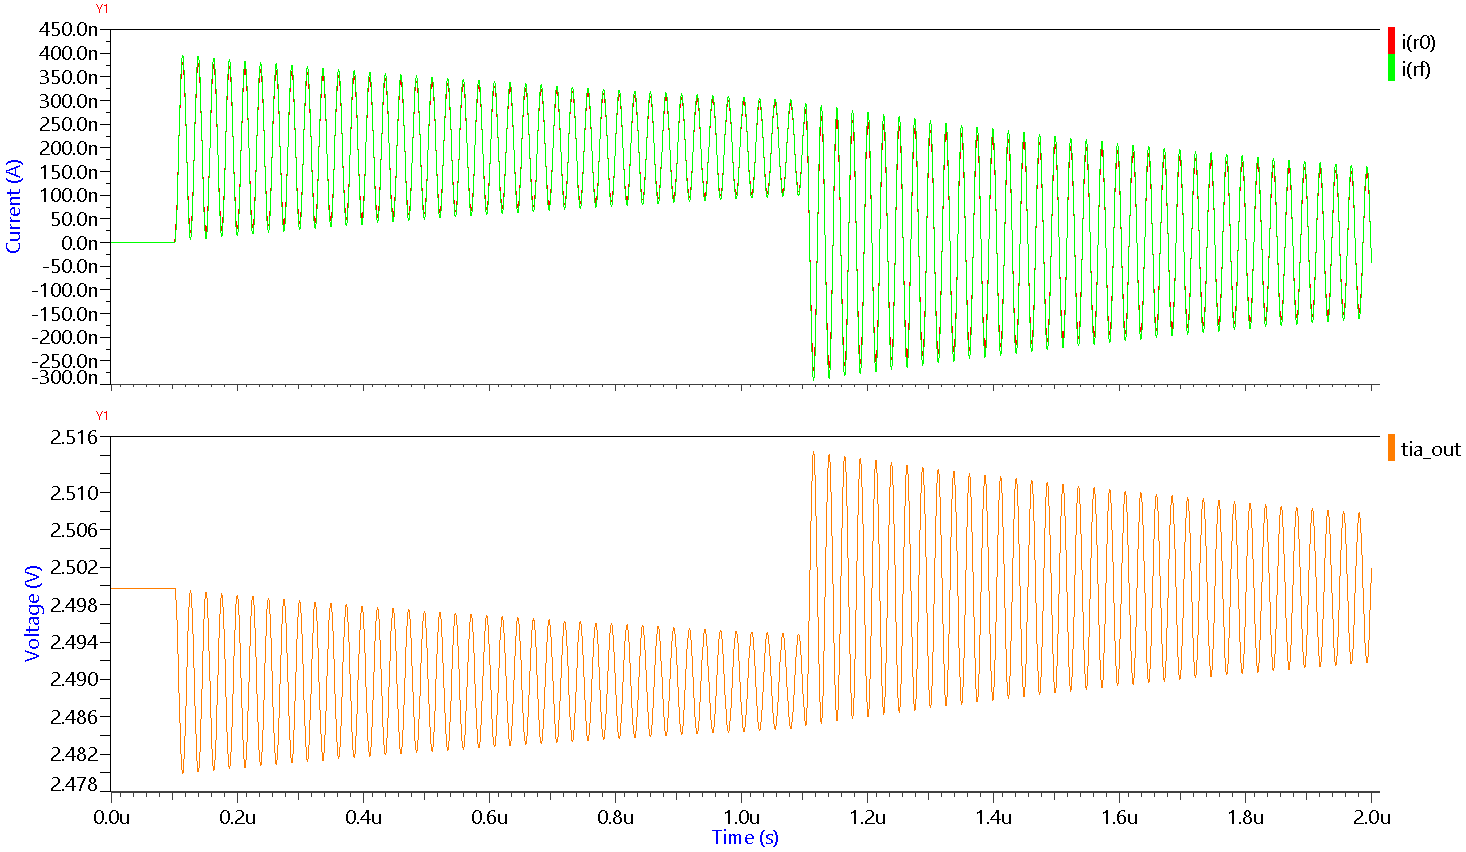
\includegraphics[width=\textwidth]{graphics/simulation_tia_plot_wo_cf.png}
    \caption{Simulation \acrshort{tia} - Plot ohne \lstinline|CF|}\label{fig:simulation_tia_plot_wo_cf}
\end{figure}

Die genaue Dimensionierung von \lstinline|CF| wird durch Tests mit dem \acrshort{pcb} bestimmt werden. Eventuell, je
nach parasitären Kapazitäten auf dem \acrshort{pcb}, wird \lstinline|CF| auch gar nicht bestückt werden müssen.

\pagebreak

\section{Umsetzung}\label{sec:realisation}
In diesem Kapitel wird die Umsetzung des Demonstrators dokumentiert.

Im Anhang~\ref{sec:photos} sind Fotos des Demonstrators abgelegt.

\pagebreak

\subsection{Firmware}

Der selbst entwickelte Firmware-Treiber für den \acrshort{tdc} befindet im Anhang~\ref{sec:tdc_driver}.

\pagebreak

\subsection{Schaltungen}
Nachfolgend werden sämtliche Teil-Schaltungen thematisiert, welche für das entwickelten \acrshort{tof}-Evaluationsmodul
nötig sind. Ein vollständiges Schema kann dem Anhang~\ref{sec:schematic_apdx} entnommen werden. Die kompletten
Projekt-Dateien sind im elektronischen Anhang dieses Projektes verfügbar.

Designt wurde das Schema mit Hilfe des Open-Source Tools \dq KiCad EDA 8.0\dq.

\subsubsection{Selective Input Voltage}

Abbildung~\ref{fig:selective_input_voltage} zeigt die Beschaltung zur Selektion der Speisung.

\begin{figure}[H]
    \centering
    \includegraphics[page=2, trim=80 590 750 50, clip, width=0.9\textwidth]{attachments/schematic.pdf}
    \caption{Selective Input Voltage}\label{fig:selective_input_voltage}
\end{figure}

Für die Speisung des Nucleo-Boards bestehen die folgenden Möglichkeiten:

\begin{itemize}
    \item 5~V von USB-Buchse
    \item 5~V von externem Power-Supply (\lstinline|JP1| + \lstinline|JP2|)
    \item 12~V von externem Power-Supply (\lstinline|JP3|)
\end{itemize}

Siehe dazu auch Kapitel~\ref{sec:schematic_nucleo}.

Für die Speisung der 5~V Elektronik bestehen die folgenden Möglichkeiten:

\begin{itemize}
    \item 5~V von Nucleo-Board (\lstinline|JP1|)
    \item 5~V von externem Power-Supply (\lstinline|JP2|)
    \item 12~V von externem Power-Supply via Nucleo-Board (\lstinline|JP1| + \lstinline|JP3|)
\end{itemize}

Für die Speisung der Photodiode bestehen die folgenden Möglichkeiten:

\begin{itemize}
    \item 5~V von 5~V-Elektronik (\lstinline|SW2| Position 3)
    \item 12~V von externem Power-Supply (\lstinline|SW2| Position 1)
\end{itemize}

Siehe dazu auch Kapitel~\ref{sec:schematic_photo_receiver}.

\subsubsection{Nucleo Board}\label{sec:schematic_nucleo}

Die Beschaltung des NUCLEO-F042K6 Boards \cite{st2024nucleof042k6_usermanual} ist in Abbildung~\ref{fig:nucleo_board}
gezeigt.

\begin{figure}[H]
    \centering
    \includegraphics[page=2, trim=530 580 300 50, clip, width=0.9\textwidth]{attachments/schematic.pdf}
    \caption{Nucleo Board}\label{fig:nucleo_board}
\end{figure}

Das NUCLEO Board ist ein sogenanntes \dq Development-Kit\dq, welches eine STM32F042K6 \acrshort{mcu}
beinhaltet. Am Rand des Boards werden diverse Pins der \acrfull{mcu} via Pin-Header
einfach zur Verfügung gestellt. Dies erleichtert die Integration in eine eigene Elektronik
enorm. Programmiert wird die \acrshort{mcu} über eine \acrshort{usb}-Schnittstelle.

In diesem Design wird das Entwicklerboard dazu benötigt, die TDC7200 ICs zu
bedienen. Dazu wird einerseits ein \acrfull{spi} benötigt, um die Mess-ICs zu konfigurieren
und auch auszulesen (siehe SPI-Bus in der Abbildung). Weiter können auf beiden \acrshort{tdc}s Messungen
gestartet werden mit den Signalen \lstinline|start_ele|, resp. \lstinline|start_opt|. Für den
\acrshort{tdc} welcher sich um die elektrischen Signale kümmert kann zudem mit \lstinline|stop_ele| ein
Stopp-Puls generiert werden.
Zu guter Letzt ist das NUCLEO dafür zuständig, die Laser-Diode anzusteuern, was mit den Signalen
\lstinline|LD_pulse| sowie $\overline{\mbox{\lstinline|LD_enable|}}$ geschieht.

\subsubsection{TDC Electrical Signal}

Die Beschaltung des TDC7200 \cite{ti2016tdc7200_datasheet} für den elektrischen Teil ist in
Abbildung~\ref{fig:tdc_ele_signal} gezeigt.

\begin{figure}[H]
    \centering
    \includegraphics[page=2, trim=80 330 750 310, clip, width=0.9\textwidth]{attachments/schematic.pdf}
    \caption{\acrshort{tdc} Electrical Signal}\label{fig:tdc_ele_signal}
\end{figure}

Der TDC7200 ist über die die Start- und Stopp-Leitungen, ein Enable-Signal sowie die \acrshort{spi}-Leitungen mit der
\acrshort{mcu} verbunden.

Wie bereits im Kapitel~\ref{sec:approach} angesprochen, wird der elektrische \acrshort{tdc} dazu verwendet, den Chip
erstmalig in Betrieb zu nehmen und sich damit vertraut zu machen. Am Anschluss \lstinline|J3| kann in einem nächsten
Schritt ein beliebig langes Kabel angeschlossen werden. Dies ermöglicht es, erste Messresultate, natürlich rein elektrisch,
vom TDC7200 auszulesen.

Mittels Schalter \lstinline|SW1| kann das \lstinline|STOP|-Signal wahlweise via \lstinline|stop_ele| oder
\lstinline|start_ele| generiert werden. Dies bietet zum einen die Möglichkeit, die Zeit zwischen dem Schalten von zwei
\acrshort{gpio}s zu messen. Zum anderen, kann derselbe \acrshort{gpio}-Pin zum Generieren des \lstinline|START|- und
\lstinline|STOP|-Signals verwendet werden, wodurch von der Verzögerungszeit direkt auf die Kabellänge an \lstinline|J3|
geschlossen werden kann.

\subsubsection{TDC Optical Signal}

Die Beschaltung des TDC7200 \cite{ti2016tdc7200_datasheet} für den optischen Teil ist in
Abbildung~\ref{fig:tdc_opt_signal} gezeigt.

\begin{figure}[H]
    \centering
    \includegraphics[page=2, trim=530 330 300 310, clip, width=0.9\textwidth]{attachments/schematic.pdf}
    \caption{\acrshort{tdc} Optical Signal}\label{fig:tdc_opt_signal}
\end{figure}

Die Beschaltung des \acrshort{tdc}s für die optische Messung gestaltet sich praktisch gleich wie beim elektrischen
Gegenstück. Der Hauptunterschied ist, hier aber, dass dessen \lstinline|STOP|-Signal nicht von der \acrshort{mcu} selber generiert
wird, sondern von einem Komparator, welcher am Ende des optischen Messpfades steht. Da der Komparator mit einem 5~V Pegel
arbeitet, ist der Spannungsteiler \lstinline|R1| / \lstinline|R2| vonnöten, welcher den 5~V Puls auf die geeigneten 3.3~V
herunterteilt.

\subsubsection{Oscillator For TDCs}

Die Beschaltung des Oszillators für die beiden \acrshort{tdc} ist in Abbildung~\ref{fig:oscillator_tdc} gezeigt. Es
handelt sich hierbei um einen normalen Quartz-Oszillator mit integriertem Schwingkreis. Praktischerweise ist bei diesem
also keine weitere Beschaltung notwendig.

\begin{figure}[H]
    \centering
    \includegraphics[page=2, trim=80 90 930 550, clip, width=0.45\textwidth]{attachments/schematic.pdf}
    \caption{Oscillator for \acrshort{tdc}s}\label{fig:oscillator_tdc}
\end{figure}

\subsubsection{Power Supply Separation}

Für die Beschaltung der Photodiode, inkl. \acrshort{tia} und Komparator, macht es Sinn eine Spannungsversorgung mit
möglichst wenig Rauschen zu haben.

Dazu wurde die Separierung vorgenommen, welche in Abbildung~\ref{fig:power_supply_separation} dargestellt ist.

\begin{figure}[H]
    \centering
    \includegraphics[page=2, trim=260 90 640 550, clip, width=0.7\textwidth]{attachments/schematic.pdf}
    \caption{Power Supply Separation}\label{fig:power_supply_separation}
\end{figure}

Prinzipiell sollen die Speisungen über eine Ferrit-Perle etwas entstört werden. Massgeblich ist hier natürlich auch der
physikalische Verlauf des Speisungspfades auf dem Layout. Dazu mehr im entsprechenden Kapitel~\ref{sec:layout}. Wahlweise
besteht nebst den Ferrit-Perlen die Möglichkeit, mittels Kondensatoren die Speisung weiter zu entkoppeln. Es wird jedoch
davon ausgegangen, dass dies in einem ersten Schritt nicht notwendig ist.

\subsubsection{Laser Driver}

Die Laser Diode RLD65NZX1 \cite{rohm2019rld65nzx1_datasheet} wird mittels Lasertreiber LMG1025-Q1 \cite{ti2024lmg1025q1_datasheet}
und NexFET \cite{ti2016csd17578q3a_datasheet} angesteuert. Für die Generierung eines kurzen Pulses (0.5 \dots 100~ns)
wurde mittels Hochpass und AND-Gatter \cite{diodes202074lvc1g08q_datasheet} implementiert. Siehe dazu Abbildung~\ref{fig:laser_driver}.

Der Widerstand \lstinline|R25| bildet den Vorwiderstand für die Laser-Diode, welcher sich gemäss der Formel~\ref{eq:ld_resistor} berechnet.

\begin{equation}\label{eq:ld_resistor}
    R_{v} = \frac{V_{cc} - V_{fld}}{I_{ld}} = \frac{5~V - 2~V}{40~mA} = 75~\Omega
\end{equation}

Im Schema eingezeichnet ist aktuell ein Platzhalterwert. Während der Inbetriebnahme wird der Widerstand je nach Bedarf
verändert. Wird dieser beispielsweise verkleinert, so vergrössert sich der Strom durch die Laser-Diode und somit die ausgesandte
Lichtleistung.

%TODO Erwähnen was für ein Widerstand schlussendlich verwendet wurde. z.B. 10x Überansteuerung weil kleiner Duty-Cycle.

\begin{figure}[H]
    \centering
    \includegraphics[page=3, trim=100 520 550 60, clip, width=0.9\textwidth]{attachments/schematic.pdf}
    \caption{Laser Driver}\label{fig:laser_driver}
\end{figure}

\subsubsection{Photo Receiver}\label{sec:schematic_photo_receiver}

Um den Photostrom der Photodiode NJL6401R \cite{jrc2014njl6401r3_datasheet} zu verstärken und in eine Spannung umzuwandeln,
wurde mit dem Operationsverstärker OPA858 \cite{ti2018opa858_datasheet} ein Transimpedanzverstärker aufgebaut. Der
Ausgang des Transimpedanzverstärkers geht auf den Komparator TLV3501 \cite{ti2016tlv3501_datasheet}, um das \lstinline|STOP|-Signal
für den \acrshort{tdc} zu generieren. Siehe dazu Abbildung~\ref{fig:photo_receiver}.

Der Feedback-Widerstand \lstinline|R26| kann je nach bedarf verändert werden. Wird dieser vergrössert, so steigt auch der
negative Puls am Ausgang des \acrshort{tia}s. Mit \lstinline|C20| kann zudem bei Bedarf eine kleine Kapazität hinzugefügt
werden. Diese hat zum Ziel, ein Schwingen des Verstärkers zu unterdrücken, falls dieser eine Neigung zum Schwingen haben
sollte.

\begin{figure}[H]
    \centering
    \includegraphics[page=3, trim=100 240 600 340, clip, width=0.9\textwidth]{attachments/schematic.pdf}
    \caption{Photo Receiver}\label{fig:photo_receiver}
\end{figure}

\subsubsection{Decoupling Capacitors}

Die Beschaltung der Entkopplungs-Kondensatoren ist in Abbildung~\ref{fig:decoupling_capacitors} dargestellt. Die
Kondensatoren für den Operationsverstärker OPA858 und für den Komparator TLV3501 wurden dem Vorschlag im Datenblatt
entnommen. Zusätzlich wird auch der Gate-Treiber beim Laser-Treiber mit einer zusätzlichen, grösseren Kapazität gestützt,
was sich positiv auf die Stabilität der Speisung auswirken sollte.

\begin{figure}[H]
    \centering
    \includegraphics[page=3, trim=100 60 650 630, clip, width=0.9\textwidth]{attachments/schematic.pdf}
    \caption{Decoupling Capacitors}\label{fig:decoupling_capacitors}
\end{figure}

\pagebreak

\subsection{Layout}\label{sec:layout}

In diesem Kapitel werden die \acrshort{pcb}-Layouts dokumentiert.

\subsubsection{Kupfer-Layer}

\begin{figure}[H]
    \centering
    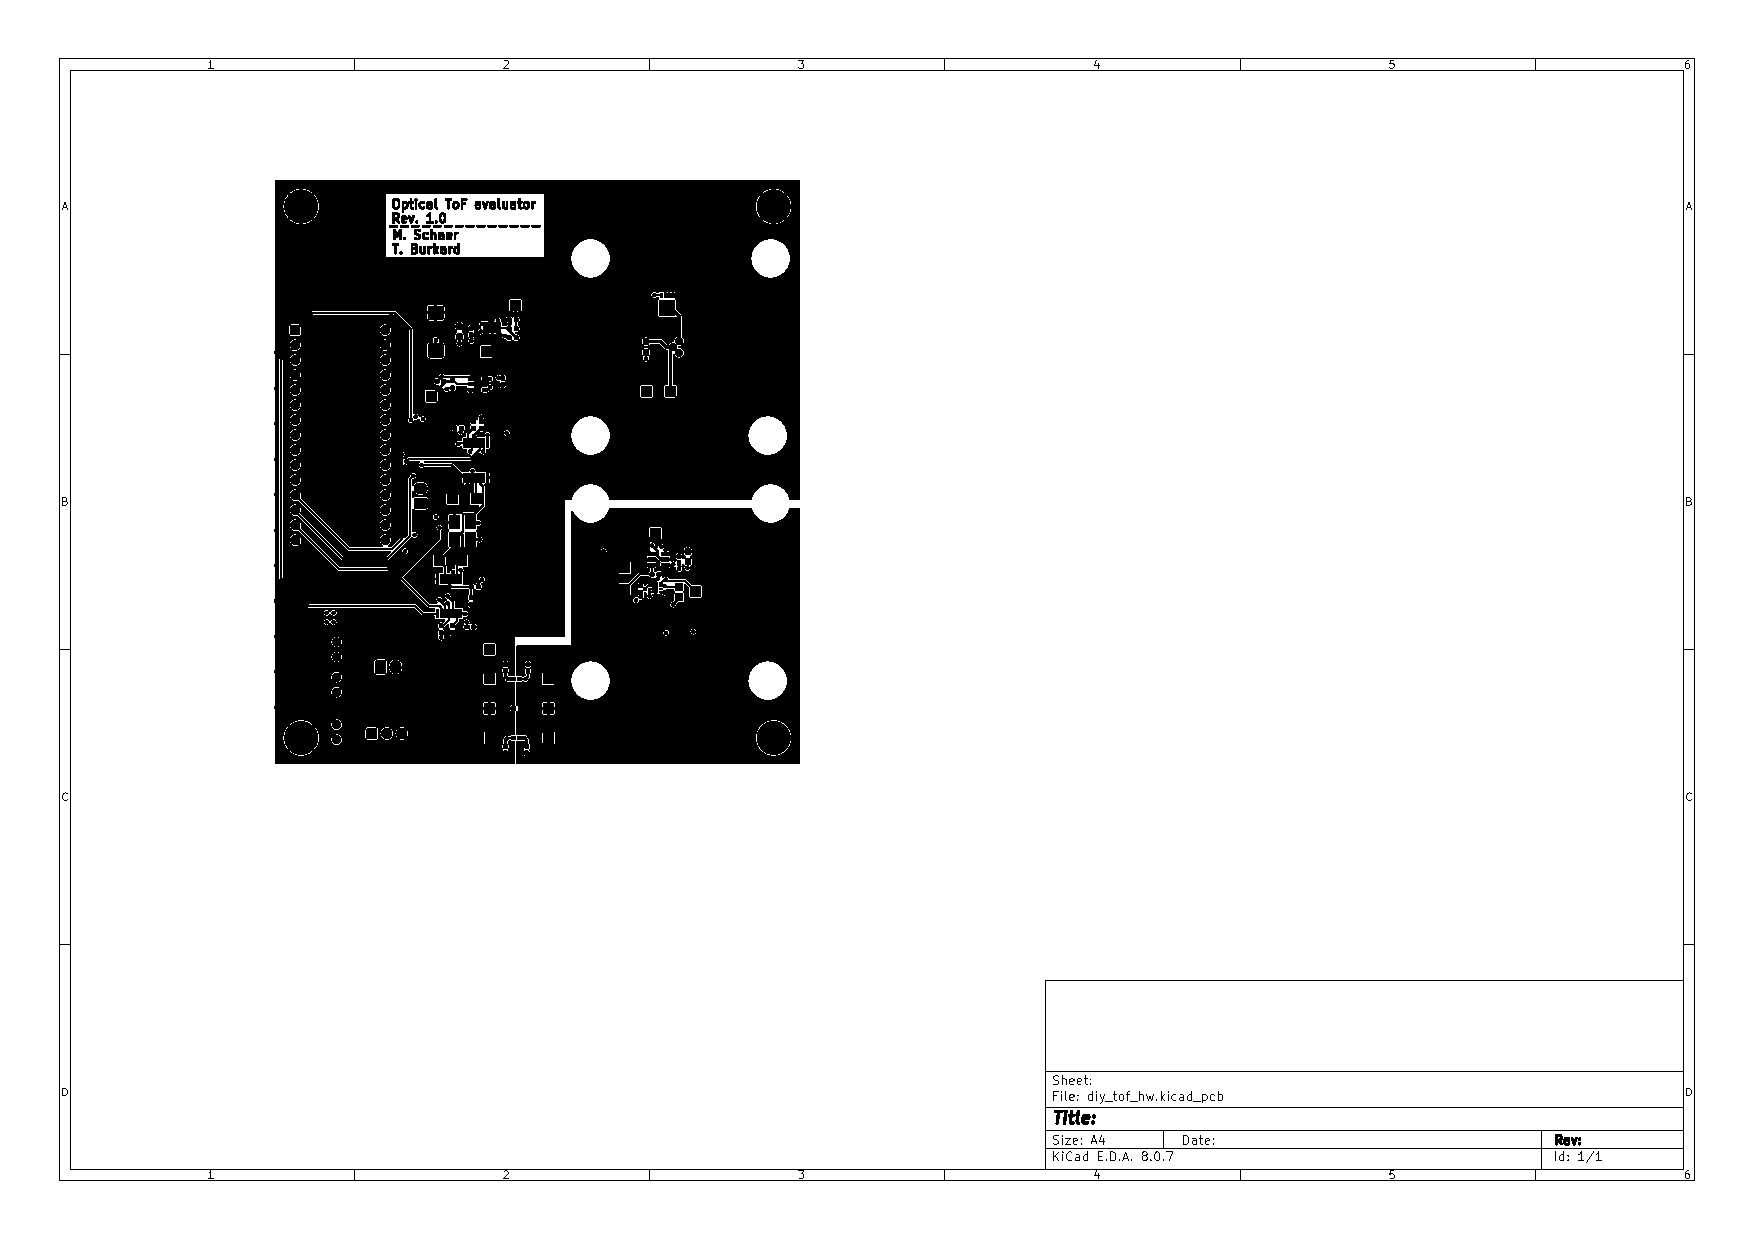
\includegraphics[trim=130 220 450 80, clip, width=0.6\textwidth]{attachments/pcb_F_Cu.pdf}
    \caption{PCB Layout Top}\label{fig:pcb_f_cu}
\end{figure}

\begin{figure}[H]
    \centering
    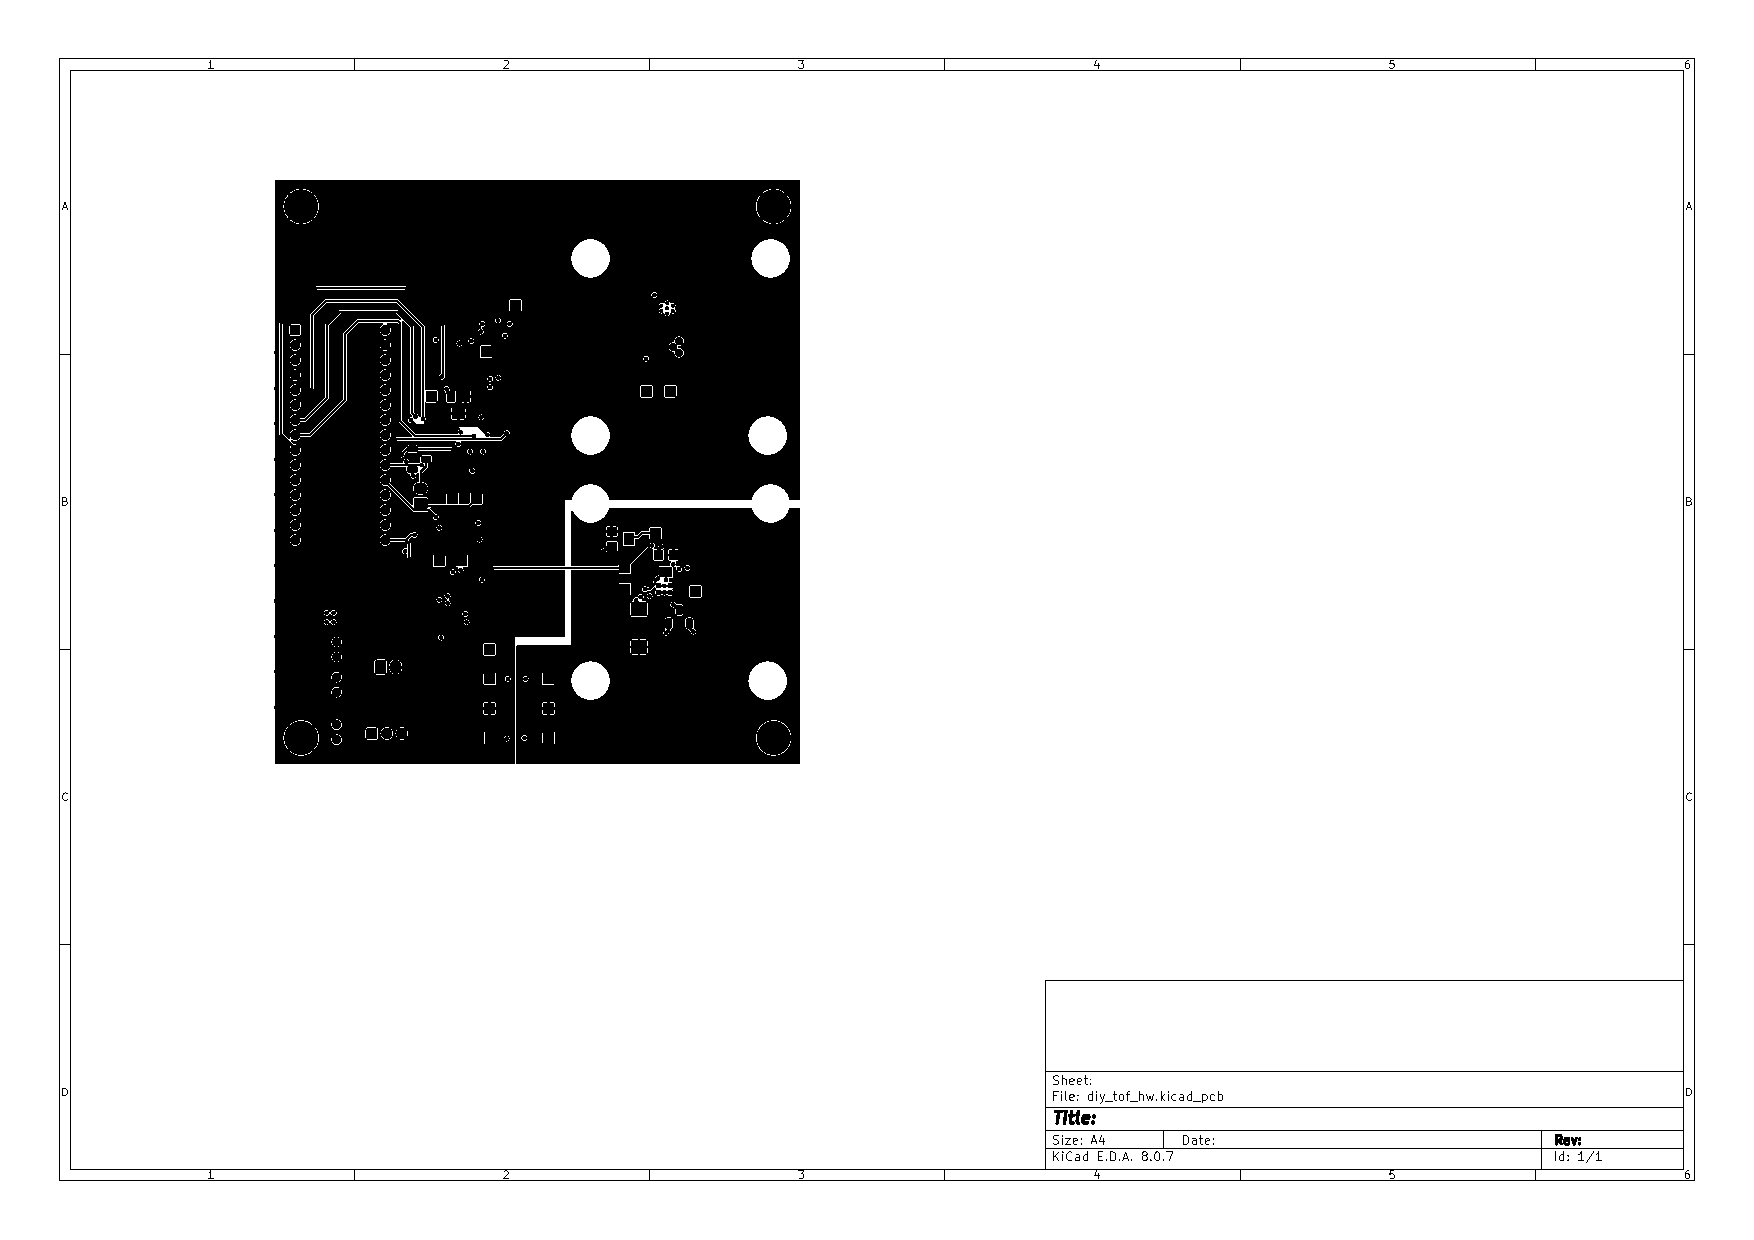
\includegraphics[trim=130 220 450 80, clip, width=0.6\textwidth]{attachments/pcb_B_Cu.pdf}
    \caption{PCB Layout Bottom}\label{fig:pcb_b_cu}
\end{figure}

\begin{figure}[H]
    \centering
    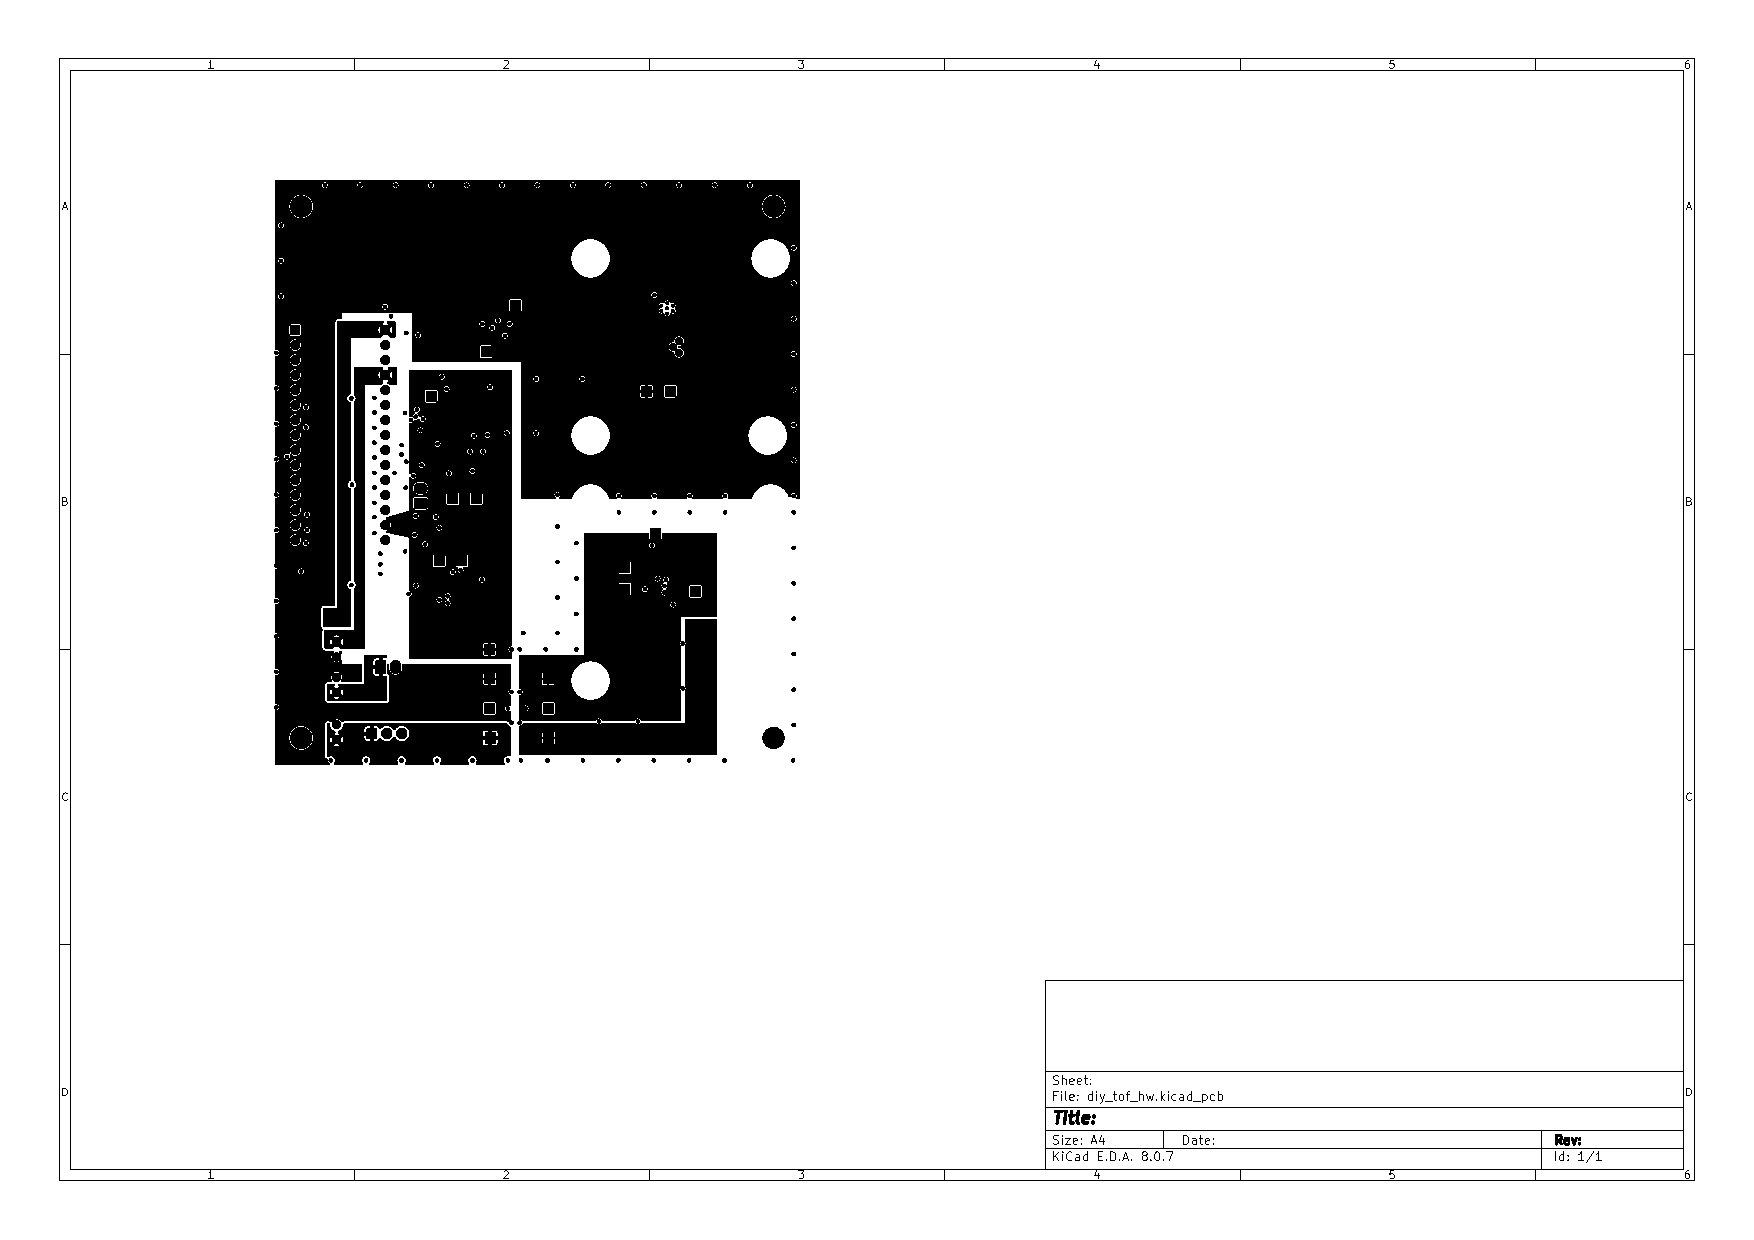
\includegraphics[trim=130 220 450 80, clip, width=0.6\textwidth]{attachments/pcb_In1_Cu.pdf}
    \caption{PCB Layout Innen 1}\label{fig:pcb_in1_cu}
\end{figure}

\begin{figure}[H]
    \centering
    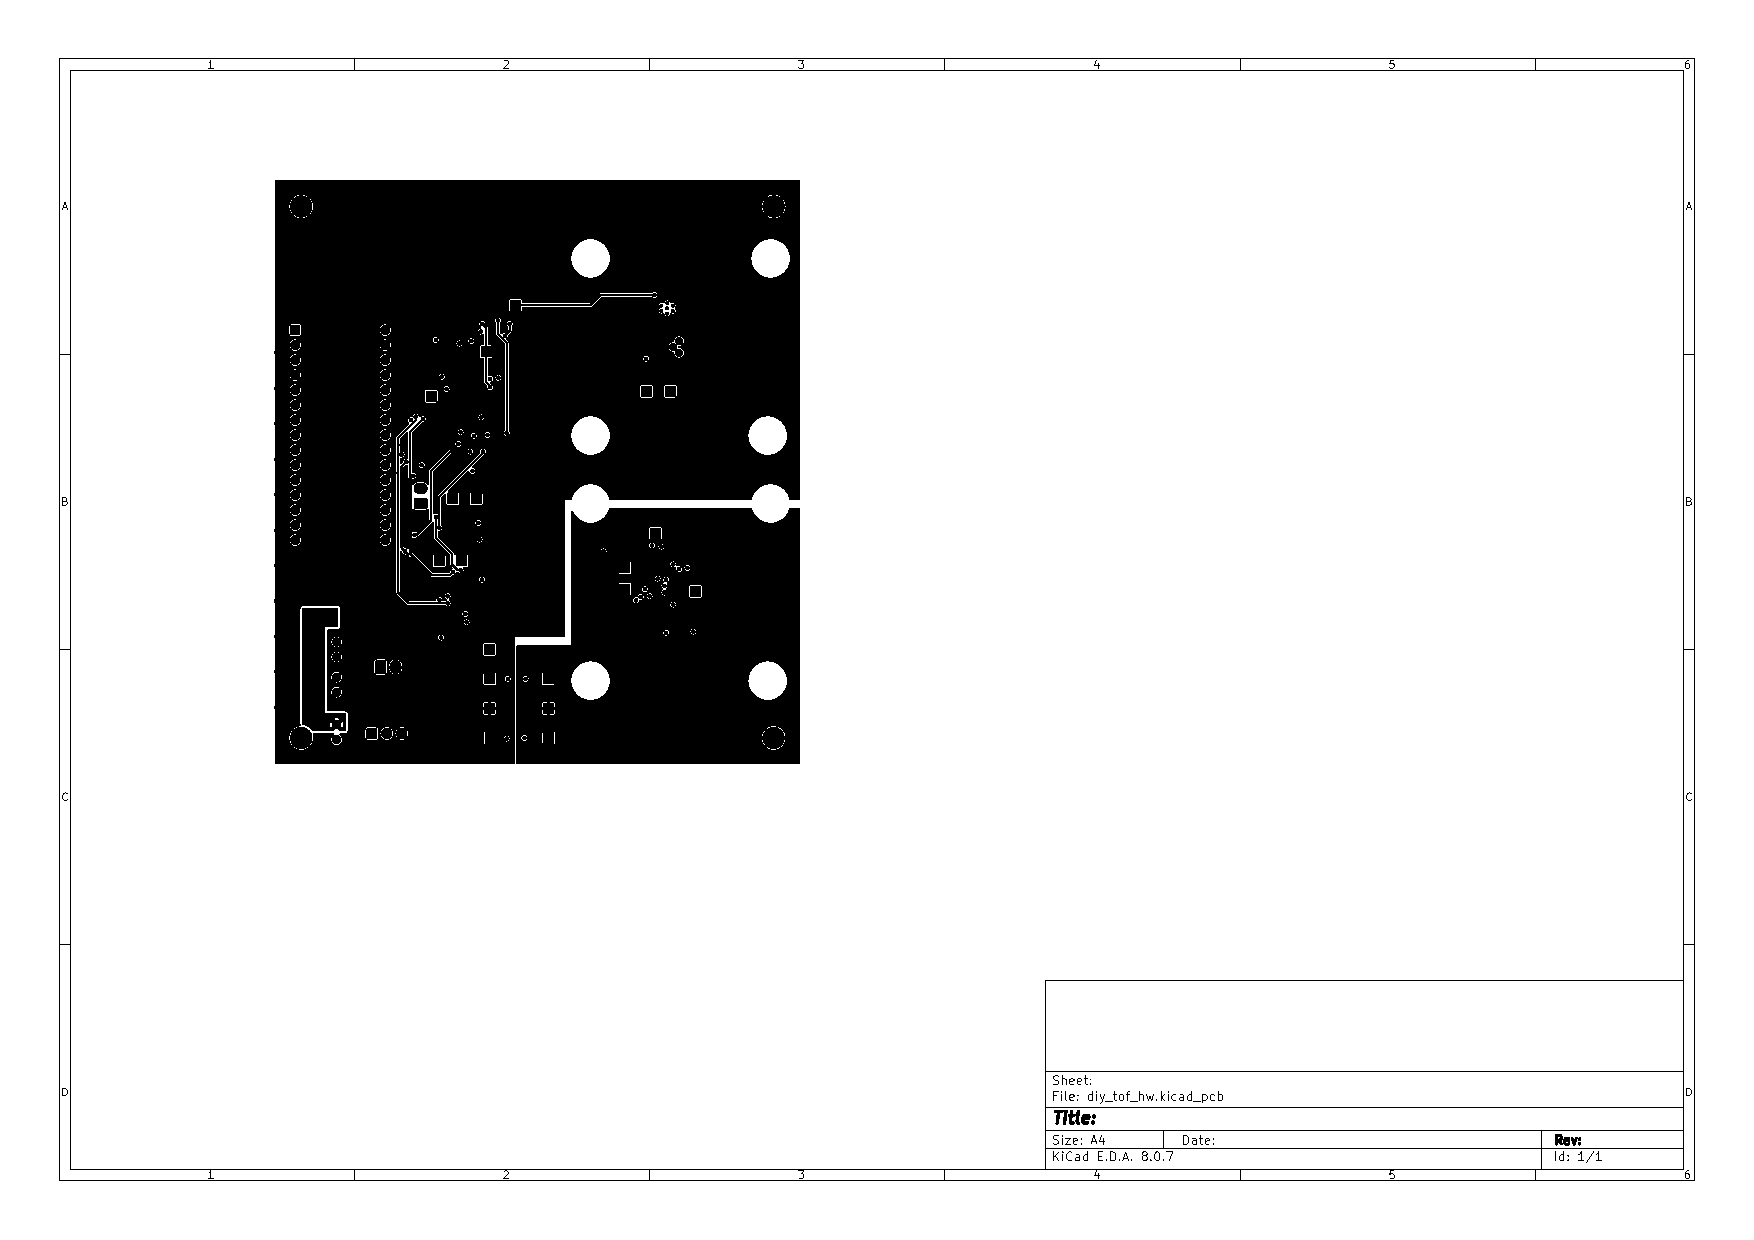
\includegraphics[trim=130 220 450 80, clip, width=0.6\textwidth]{attachments/pcb_In2_Cu.pdf}
    \caption{PCB Layout Innen 2}\label{fig:pcb_in2_cu}
\end{figure}

\subsubsection{Komponenten-Platzierung}

\begin{figure}[H]
    \centering
    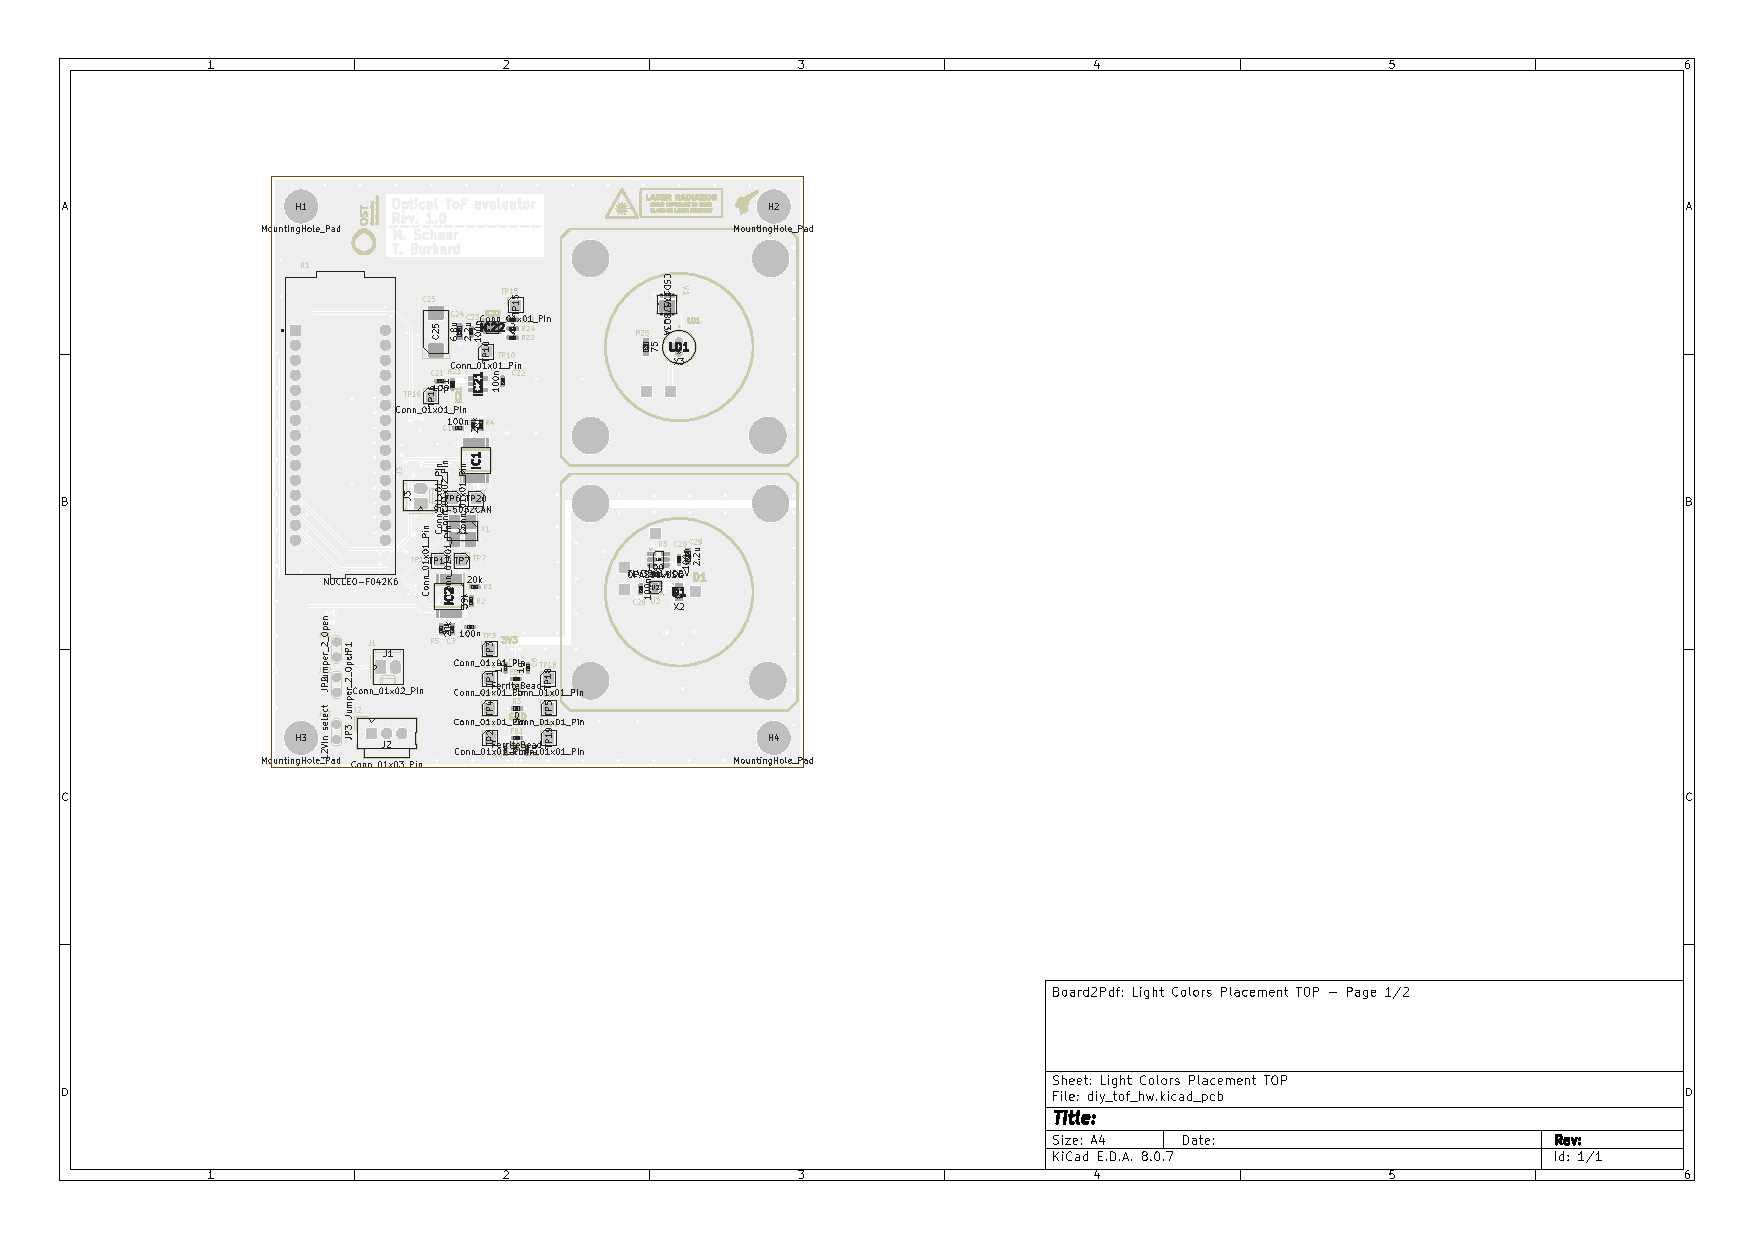
\includegraphics[page=1, trim=120 220 450 80, clip, width=0.6\textwidth]{attachments/pcb_placement.pdf}
    \caption{PCB Komponenten-Platzierung Top}\label{fig:pcb_placement_1}
\end{figure}

\begin{figure}[H]
    \centering
    \includegraphics[page=2, trim=450 220 120 80, clip, width=0.6\textwidth]{attachments/pcb_placement.pdf}
    \caption{PCB Komponenten-Platzierung Bottom}\label{fig:pcb_placement_2}
\end{figure}

\pagebreak

\subsection{3D View}

\begin{figure}[H]
    \centering
    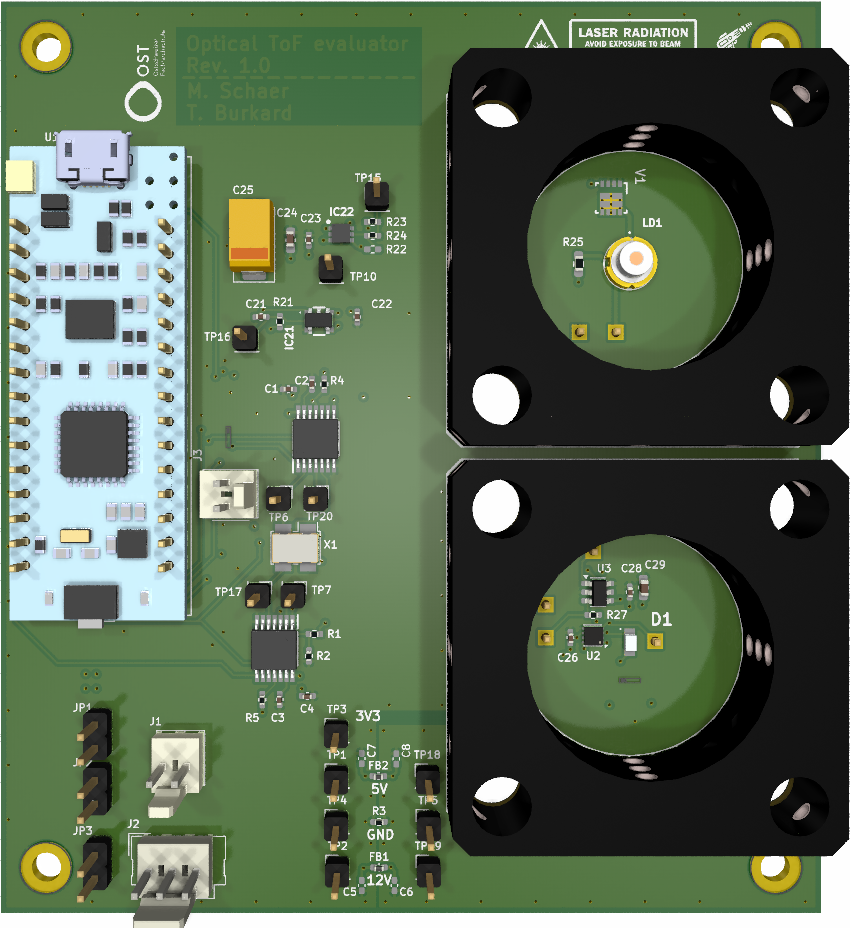
\includegraphics[width=0.6\textwidth]{graphics/3d_top.png}
    \caption{3D View Top}\label{fig:3d_top}
\end{figure}

\begin{figure}[H]
    \centering
    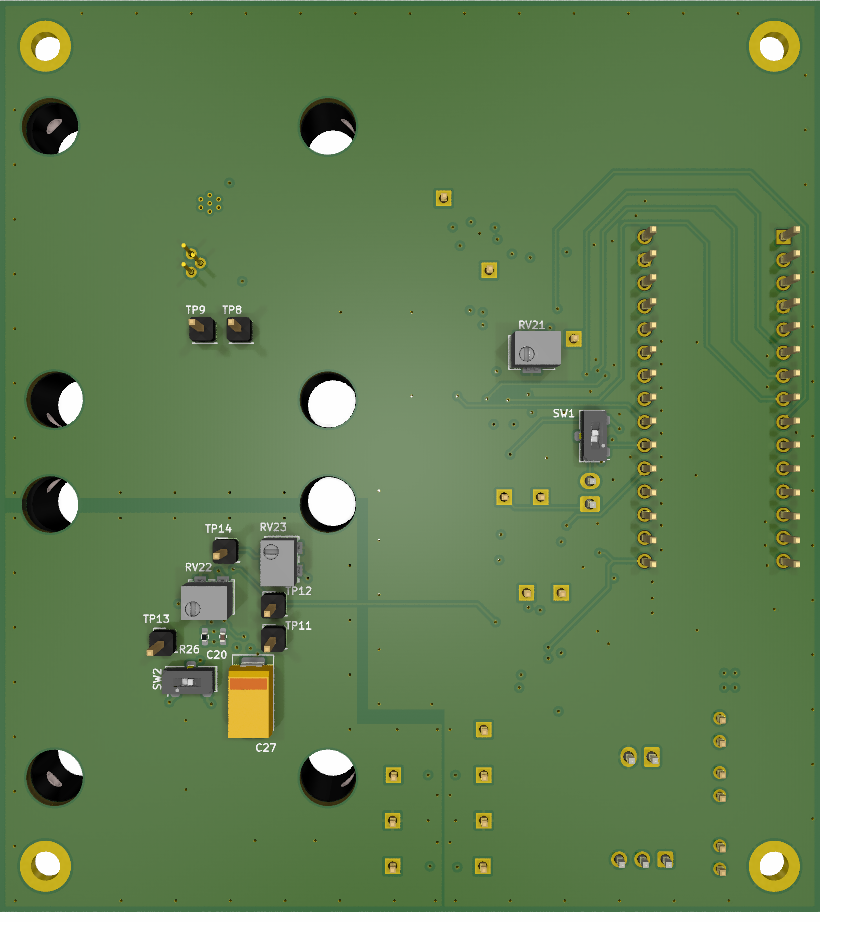
\includegraphics[width=0.6\textwidth]{graphics/3d_bottom.png}
    \caption{3D View Bottom}\label{fig:3d_bottom}
\end{figure}

\pagebreak

\section{Resultate}\label{sec:results}
\subsection{Elektrische Resultate}

\begin{frame}{Unterschiedliche Kabellängen}
    \begin{figure}
        \includesvg[width=0.8\textwidth]{../documentation/graphics/different_cable_lengths_with_dso_tdc.svg}
    \end{figure}
\end{frame}

\begin{frame}{Unterschiedliche Kabellängen: Resultate}
    \begin{table}
        \mytable
            {|l|l|l|l|}
            {\textbf{Länge} & \textbf{Mittelwert} & \textbf{Standardabweichung} & \textbf{$\Delta$ zu 0~m}}
            {\length & \mean & \stddev & \diff}
            {../documentation/tables/different_cable_lengths_with_dso_tdc.csv}
    \end{table}
\end{frame}

\begin{frame}{Unterschiedliche Kabellängen: Zurückgerechnet}
    \begin{table}
        \mytable
            {|l|l|}
            {\textbf{Länge} & \textbf{TDC zurückgerechnet mit 0.9~c}}
            {\length & \tdcgemtheoriemc}
            {../documentation/tables/different_cable_lengths_with_dso_theorie09_vs_tdc_m.csv}
    \end{table}
\end{frame}

\subsection{Optische Resultate}

\begin{frame}{Signalpfad Sender}
    \begin{figure}
        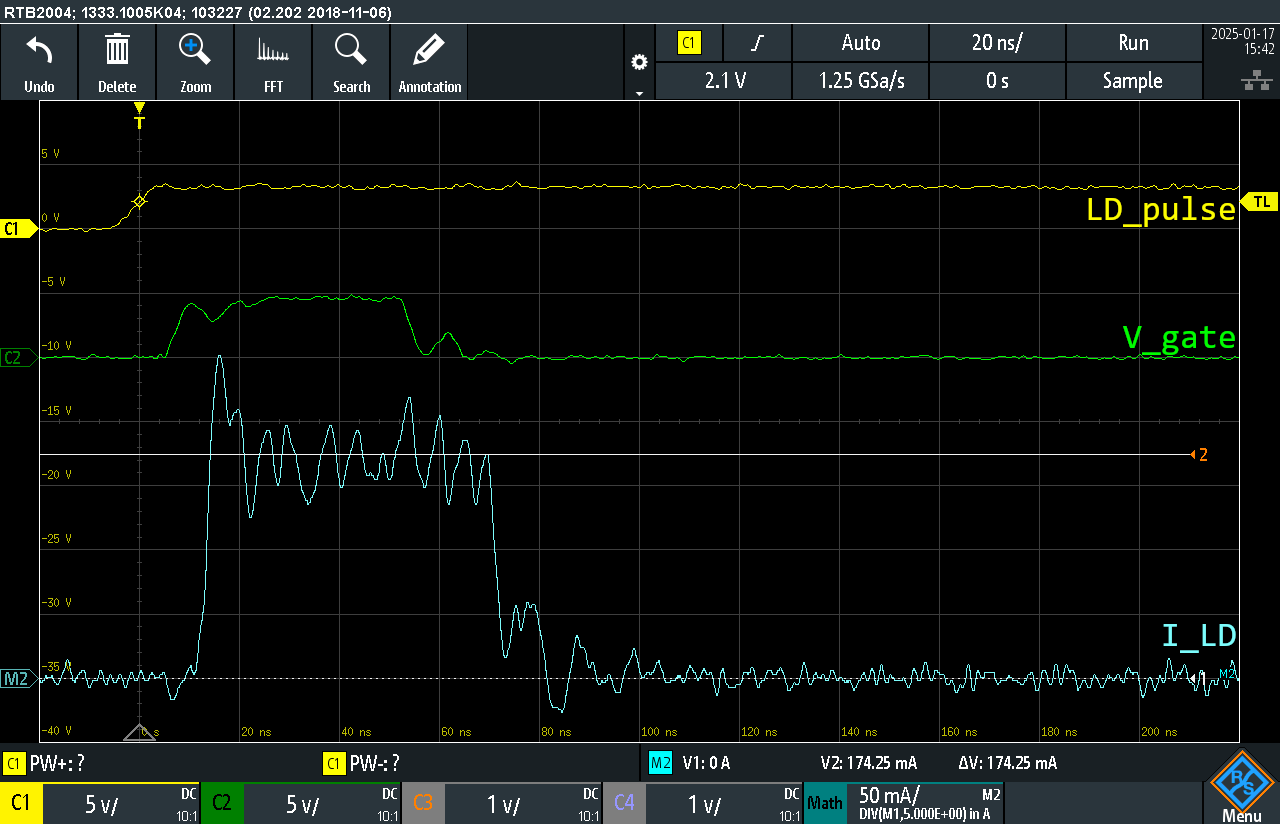
\includegraphics[width=0.7\textwidth]{../documentation/graphics/signalpfad_sender_ld_strom.png}
    \end{figure}
\end{frame}

\begin{frame}{ToF-Messungen via Spiegel}
    \begin{figure}
        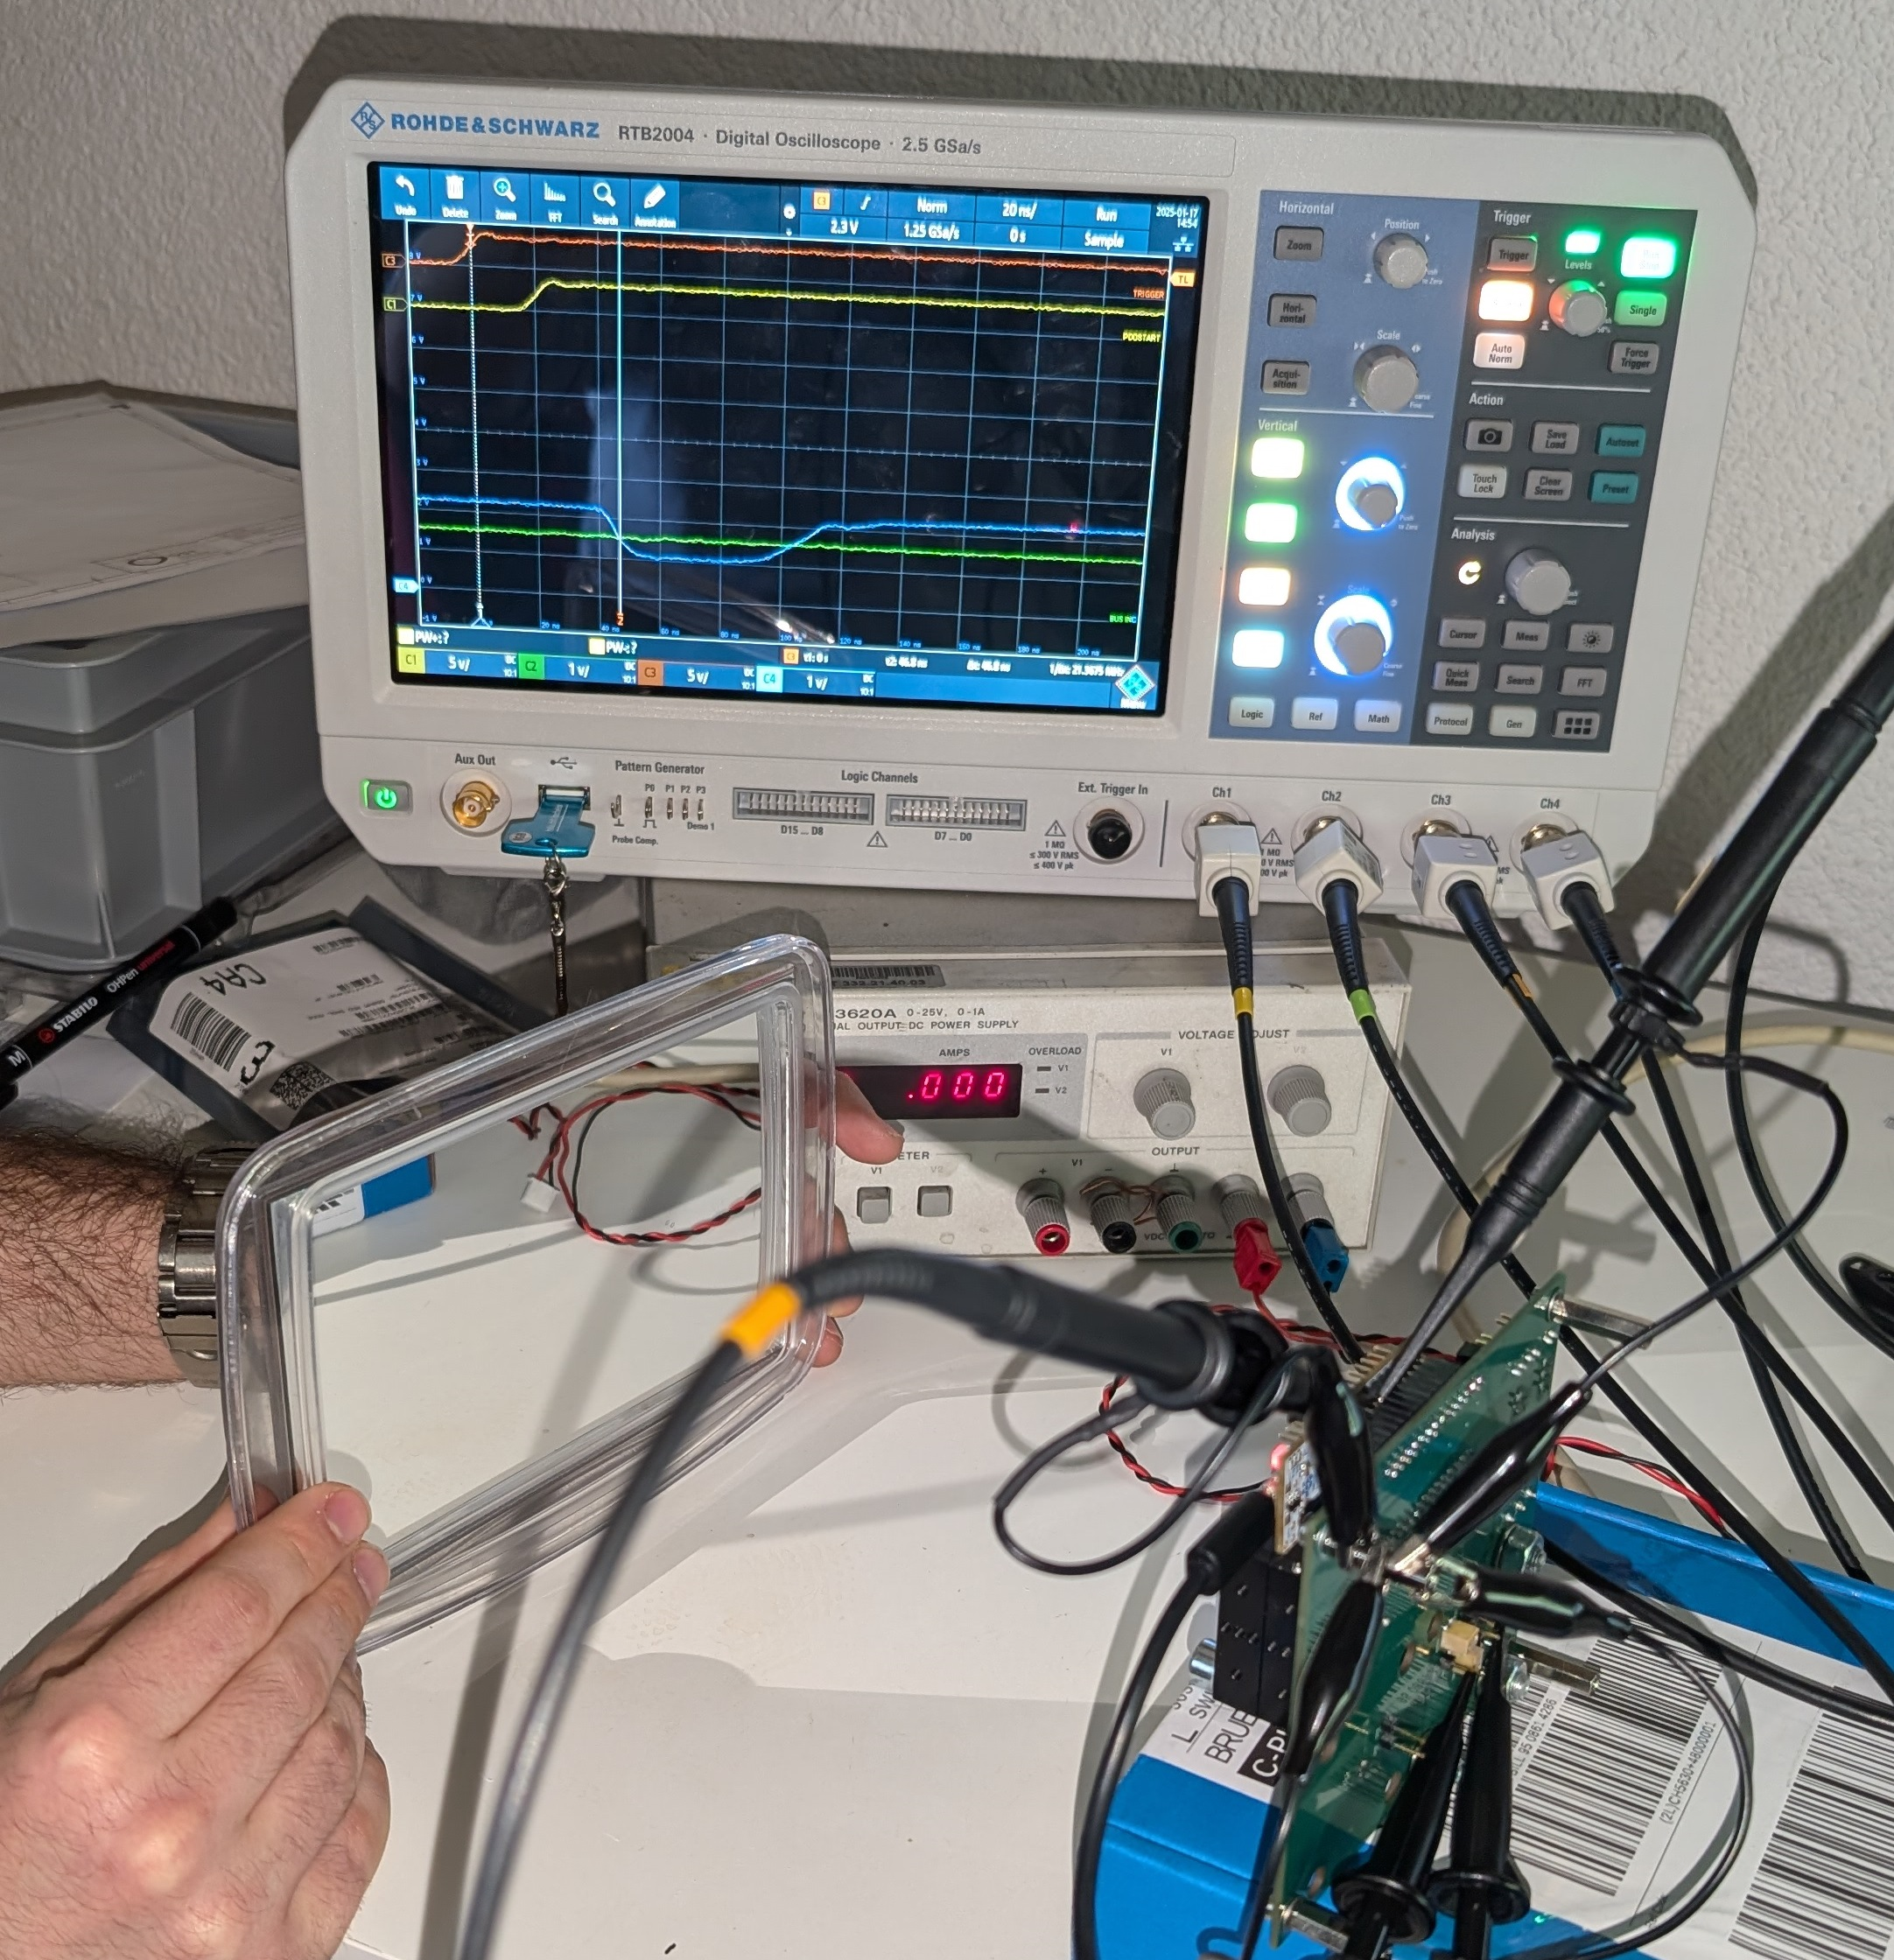
\includegraphics[width=0.45\textwidth]{../documentation/graphics/spiegel_setup.jpg}
    \end{figure}
\end{frame}

\begin{frame}{ToF-Messungen via Spiegel: DSO}
    \begin{figure}
        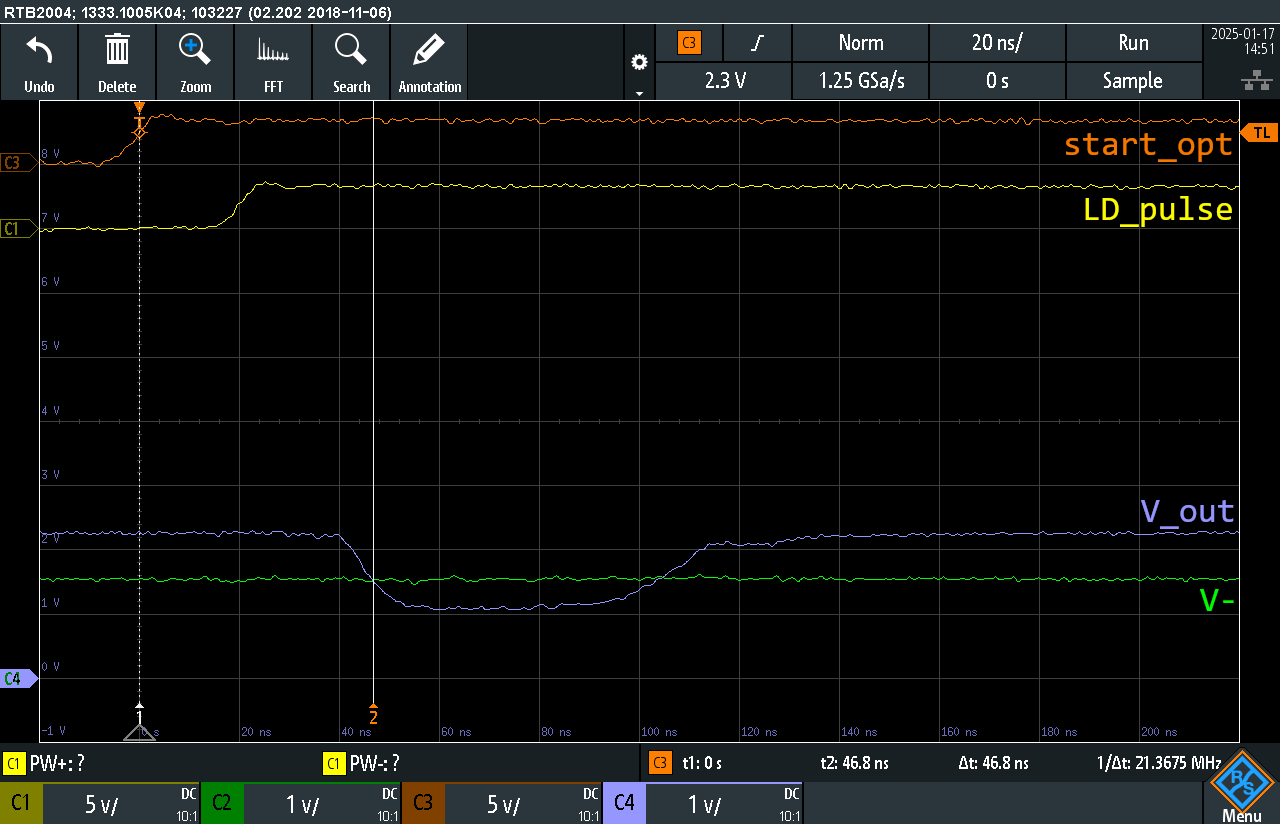
\includegraphics[width=0.7\textwidth]{../documentation/graphics/spiegel_12cm_dso_ok.png}
    \end{figure}
\end{frame}

\begin{frame}{ToF-Messungen via Spiegel: Resultate}
    \begin{figure}
        \includesvg[width=0.8\textwidth]{../documentation/graphics/spiegel_unterschiedliche_distanzen.svg}
    \end{figure}
\end{frame}

\begin{frame}{ToF-Messungen via Spiegel: Auswertung}
    \begin{table}
        \mytable
            {|l|l|l|}
            {\textbf{Distanz zum Spiegel} & \textbf{Mittelwert} & \textbf{Standardabweichung}}
            {\distance & \mean & \stddev}
            {../documentation/tables/spiegel_unterschiedliche_distanzen.csv}
    \end{table}

    \onslide<2->{
        \begin{equation*}
            \begin{split}
                \Delta ToF_{meas} &\approx 0.6~ns\\
                \Delta ToF_{calc} &= \frac{\Delta L}{c} = \frac{10~cm}{3 \cdot 10^8~m/s} = 0.33~ns
            \end{split}
        \end{equation*}
    }
\end{frame}

\begin{frame}{ToF-Messungen via Spiegel: Drift}
    \begin{figure}
        \includesvg[width=0.8\textwidth]{../documentation/graphics/spiegel_unterschiedliche_distanzen_linear.svg}
    \end{figure}
\end{frame}

\begin{frame}{ToF-Messungen via Spiegel: $>$30 cm}
    \begin{figure}
        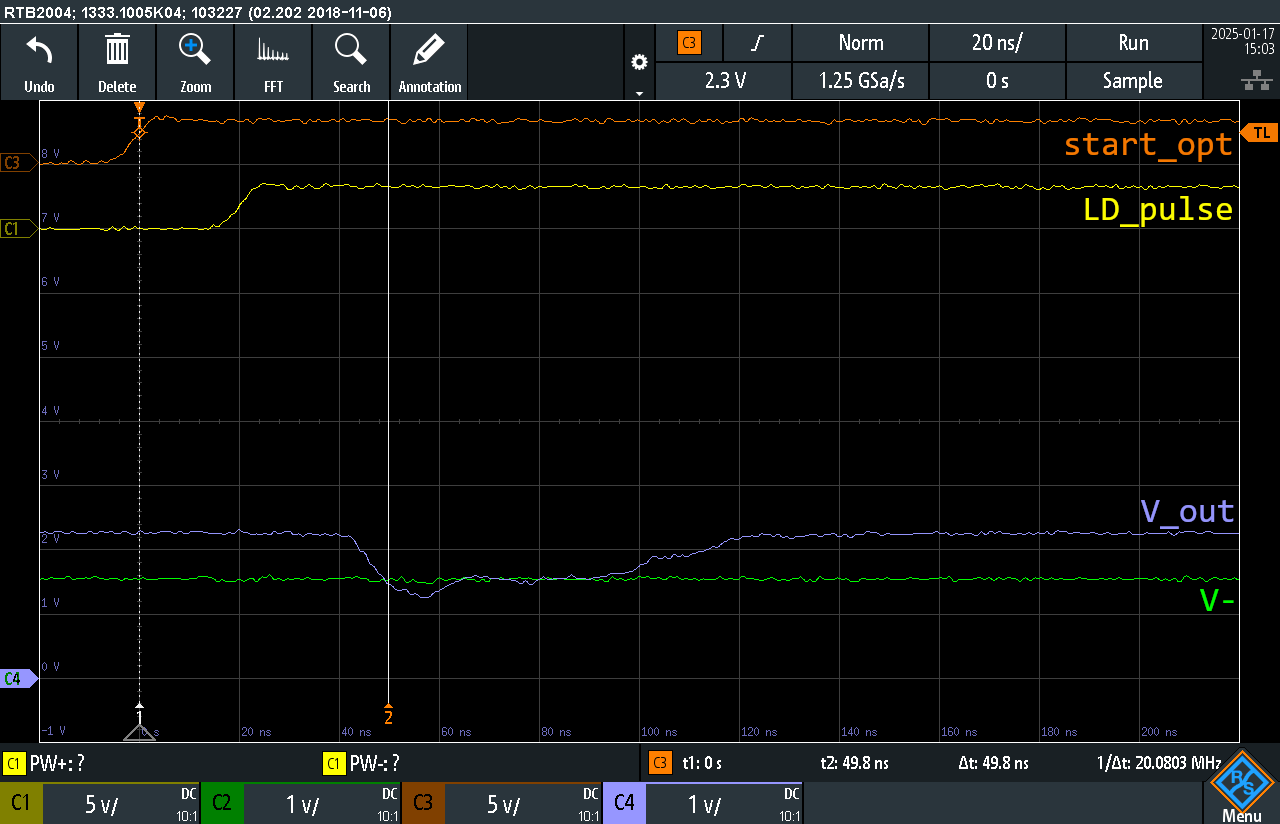
\includegraphics[width=0.7\textwidth]{../documentation/graphics/spiegel_30cm_dso_nok.png}
    \end{figure}
\end{frame}

\begin{frame}{ToF-Messungen via Wand}
    \begin{itemize}
        \item Leider keine brauchbaren Messresultate bis jetzt
    \end{itemize}
\end{frame}

\pagebreak

\section{Fazit}\label{sec:conclusion}
In diesem Kapitel werden abschliessende Gedanken gesammelt. Es soll dazu dienen einen Ausblick zu geben für mögliche,
weiterführende Arbeiten. Es sollen auch einige Punkte aufzuzählen, die gut gelaufen sind, aber auch jene bei denen
Verbesserungspotential identifiziert wurde.

\subsection{Ausblick}\label{sec:ausblick}

Grundsätzlich kann bestätigt werden, dass sich ein \acrshort{tof}-System, so wie es sich die Studierenden vorstellen,
entwickeln und betreiben lässt. Nachfolgend werden ein paar mögliche Verbesserungen und weiterführende Messungen
aufgelistet.

\begin{enumerate}
    \item Die Optik besser aufeinander abstimmen. Dies würde es zum einen erlauben, über weitere Distanzen hinweg
          Messungen machen zu können. Des weiteren sollte es ebenfalls möglich sein, auch Targets mit nicht oder schwach
          reflektierenden Oberflächen-Beschaffenheiten zu detektieren.
    \item Für die Messungen mit dem Spiegel würde es Sinn machen mit einer Linse mit grösserer Brennweite (oder mit
          derselben Linse mit etwas weniger Distanz zum \acrshort{pcb}) auszuprobieren. Dies hätte den Vorteil, dass der
          Spiegel nicht ganz so genau ausgerichtet werden muss. Der Nachteil wäre etwas weniger Photostrom bei parallel
          einfallendem Licht.
    \item Bei der Ansteuerung der \acrshort{tdc}s gibt es Verbesserungspotential. So könnte beispielsweise mit einer
          schneller getakteten \acrshort{mcu} der Jitter bei \lstinline|START|- und \lstinline|STOP|-Signal minimiert
          werden, was zu Messresultaten mit noch weniger Streuung führen wird.
    \item Eine andere Möglichkeit um die Streuung zu senken, wäre es eine externe Clock-Quelle zu verwenden.
    \item Eventuell ist es möglich auf die künstlich eingefügte Verzögerungszeit von einem Taktzyklus zu verzichten.
          Dies wäre der Fall, falls im Messpfad bereits genug Verzögerung entsteht, um die minimale Messdauer von 12~ns
          zu überschreiten. Falls nicht, könnte die künstliche Verzögerung anstatt von der \acrshort{mcu} auch mittels
          separater Schaltung (mit möglichst tiefem Jitter) umgesetzt werden.
    \item Beim verwendeten Nucleo gibt es die Möglichkeit, die Anstiegszeit der \acrshort{gpio} zu konfigurieren. Mit
          schnellerer Anstiegszeit lassen sich evtl. die Messresultate verbessern.
    \item Optischer Empfangspfad: Es sollten Messungen mit unterschiedlichen Verstärkungen des \acrshort{tia}
          durchgeführt werden, um die Distanz mit Spiegel zu erhöhen und Messungen gegen die Wand oder andere Targets zu
          ermöglichen. Damit zusammenhängend sollte die Schaltschwelle des Komparators genauer ausgetestet und
          feinjustiert werden.
    \item Optischer Sendepfad: Es lohnt sich mit höherer Sendeleistung zu experimentieren. Aufgrund der 5~V Speisung
          der Laser-Diode sind wir mit dem $5~\Omega$ Vorwiderstand schon fast am Limit. In einer nächsten
          \acrshort{pcb}-Version würde es sich lohnen mit einem Schalter die Möglichkeit zur 12~V Speisung vorzusehen,
          analog dazu wie dies für die Photodiode bereits umgesetzt ist.
    \item Optische Messungen: Es lohnt sich zu analysieren, weshalb die Messresultate in zwei Clustern (ca. 2~ns
          auseinander liegend) verteilt sind.
    \item Für weitere Messungen mit einem Spiegel lohnt es sich einen präzisen, mechanischen Versuchsaufbau zu
          konstruieren. Bei diesem könnte der Spiegel besser fixiert und eingestellt werden. Von Hand ist es schwierig
          reproduzierbare Ergebnisse zu erzielen.
\end{enumerate}

Abschliessend kann gesagt werden, dass es durchaus möglich ist, mit einem TDC7200 eine \acrshort{tof}-Messung zu machen,
bei welcher die zeitliche Auflösung des Mess-\acrshort{ic}s selber die limitierende Grösse ist.

\subsection{Lessons Learned}

Wie die Messresultate und auch der Ausblick bereits vermuten lassen, hätte primär beim Auslegen der Optoelektronik etwas
mehr Zeit investiert werden können. Die initialen, überschlags-mässigen Schätzungen und Rechnungen bezüglich der gewünschten
Limitierungen des Systems hätten kritischer hinterfragt werden sollen. Initial war es das Ziel der Studenten, Messungen
auf Distanzen von bis zu 10~m mit einer Auflösung von etwa 10~cm zu machen. Herausgestellt hat sich am Ende jedoch, dass
nicht die zeitliche Auflösung, sondern vielmehr die Distanz, resp. die Stärke des Messsignals problematisch ist.

Mit der Fabrikation des \acrshort{tof}-Demonstrators ist das Studenten-Team zufrieden. Beim erneuten Einsatz so kleiner
SMD-Komponenten, wie beispielsweise beim \acrshort{tia} lohnt es sich jedoch darüber zu sinnieren, ob nicht eine
maschinelle Bestückung der händischen Bestückung vorzuziehen ist. Durch die manuelle Bestückung wurde wohl keine Zeit
eingespart, da diese auch einige Stunden über mehrere Abende verteilt in Anspruch nahm.

\subsection{Danksagung}

Wir möchten uns an dieser Stelle herzlich bei den beiden Dozenten Prof. Guido Keel und Michael Lehmann bedanken. Während
der Laufzeit des Projekts sind sie uns jederzeit mit Rat und Tat zur Seite gestanden und haben das Projekt mit grossem
Interesse verfolgt. Auch für das optische Leihmaterial bedanken wir uns. Dieses hat uns ermöglicht, bei der optischen
Messung einen Teilerfolg erzielen zu können.

Weiter bedanken wir uns bei Robin Burkard, der für uns ein Layout-Review durchgeführt hat. Dank seinen wertvollen Tipps
konnte das \acrshort{pcb} so störfrei wie möglich in Betrieb genommen werden.

\pagebreak

\section{Anhang}\label{sec:appendix}
\subsection{TDC Treiber}\label{sec:tdc_driver}

In Code~\ref{code:tdc_driver_header} und \ref{code:tdc_driver_source} ist der selbst entwickelte Firmware-Treiber für
den \acrshort{tdc} dargestellt.

\lstinputlisting[language={c}, label={code:tdc_driver_header}, caption={\acrshort{tdc} Driver (Header)}]{../firmware/Core/TDC/TDC.h}
\lstinputlisting[language={c}, label={code:tdc_driver_source}, caption={\acrshort{tdc} Driver (Source)}]{../firmware/Core/TDC/TDC.c}

\subsection{Python Analyse}\label{sec:python_analyze}

In Code \ref{code:python_analyze} ist das Python-Skript zur Berechnung des arithmetischen Mittelwerts und der
Standardabweichung sowie zum Plotten des Histogramms und des Boxplots dargestellt.

\lstinputlisting[language={python}, label={code:python_analyze}, caption={Python Analyse}]{../utilities/analyze-tof.py}

In Code \ref{code:python_analyze_multi} ist das Python-Skript zur Berechnung des arithmetischen Mittelwerts und der
Standardabweichung sowie zum Plotten der Werte für mehrere Messungen dargestellt.

\lstinputlisting[language={python}, label={code:python_analyze_multi}, caption={Python Analyse (Multi)}]{../utilities/analyze-tofs.py}

\pagebreak

\begin{landscape}

    \subsection{Schema}\label{sec:schematic_apdx}
    \global\pdfpageattr\expandafter{\the\pdfpageattr/Rotate 90}
    \begin{figure}[H]
        \centering
        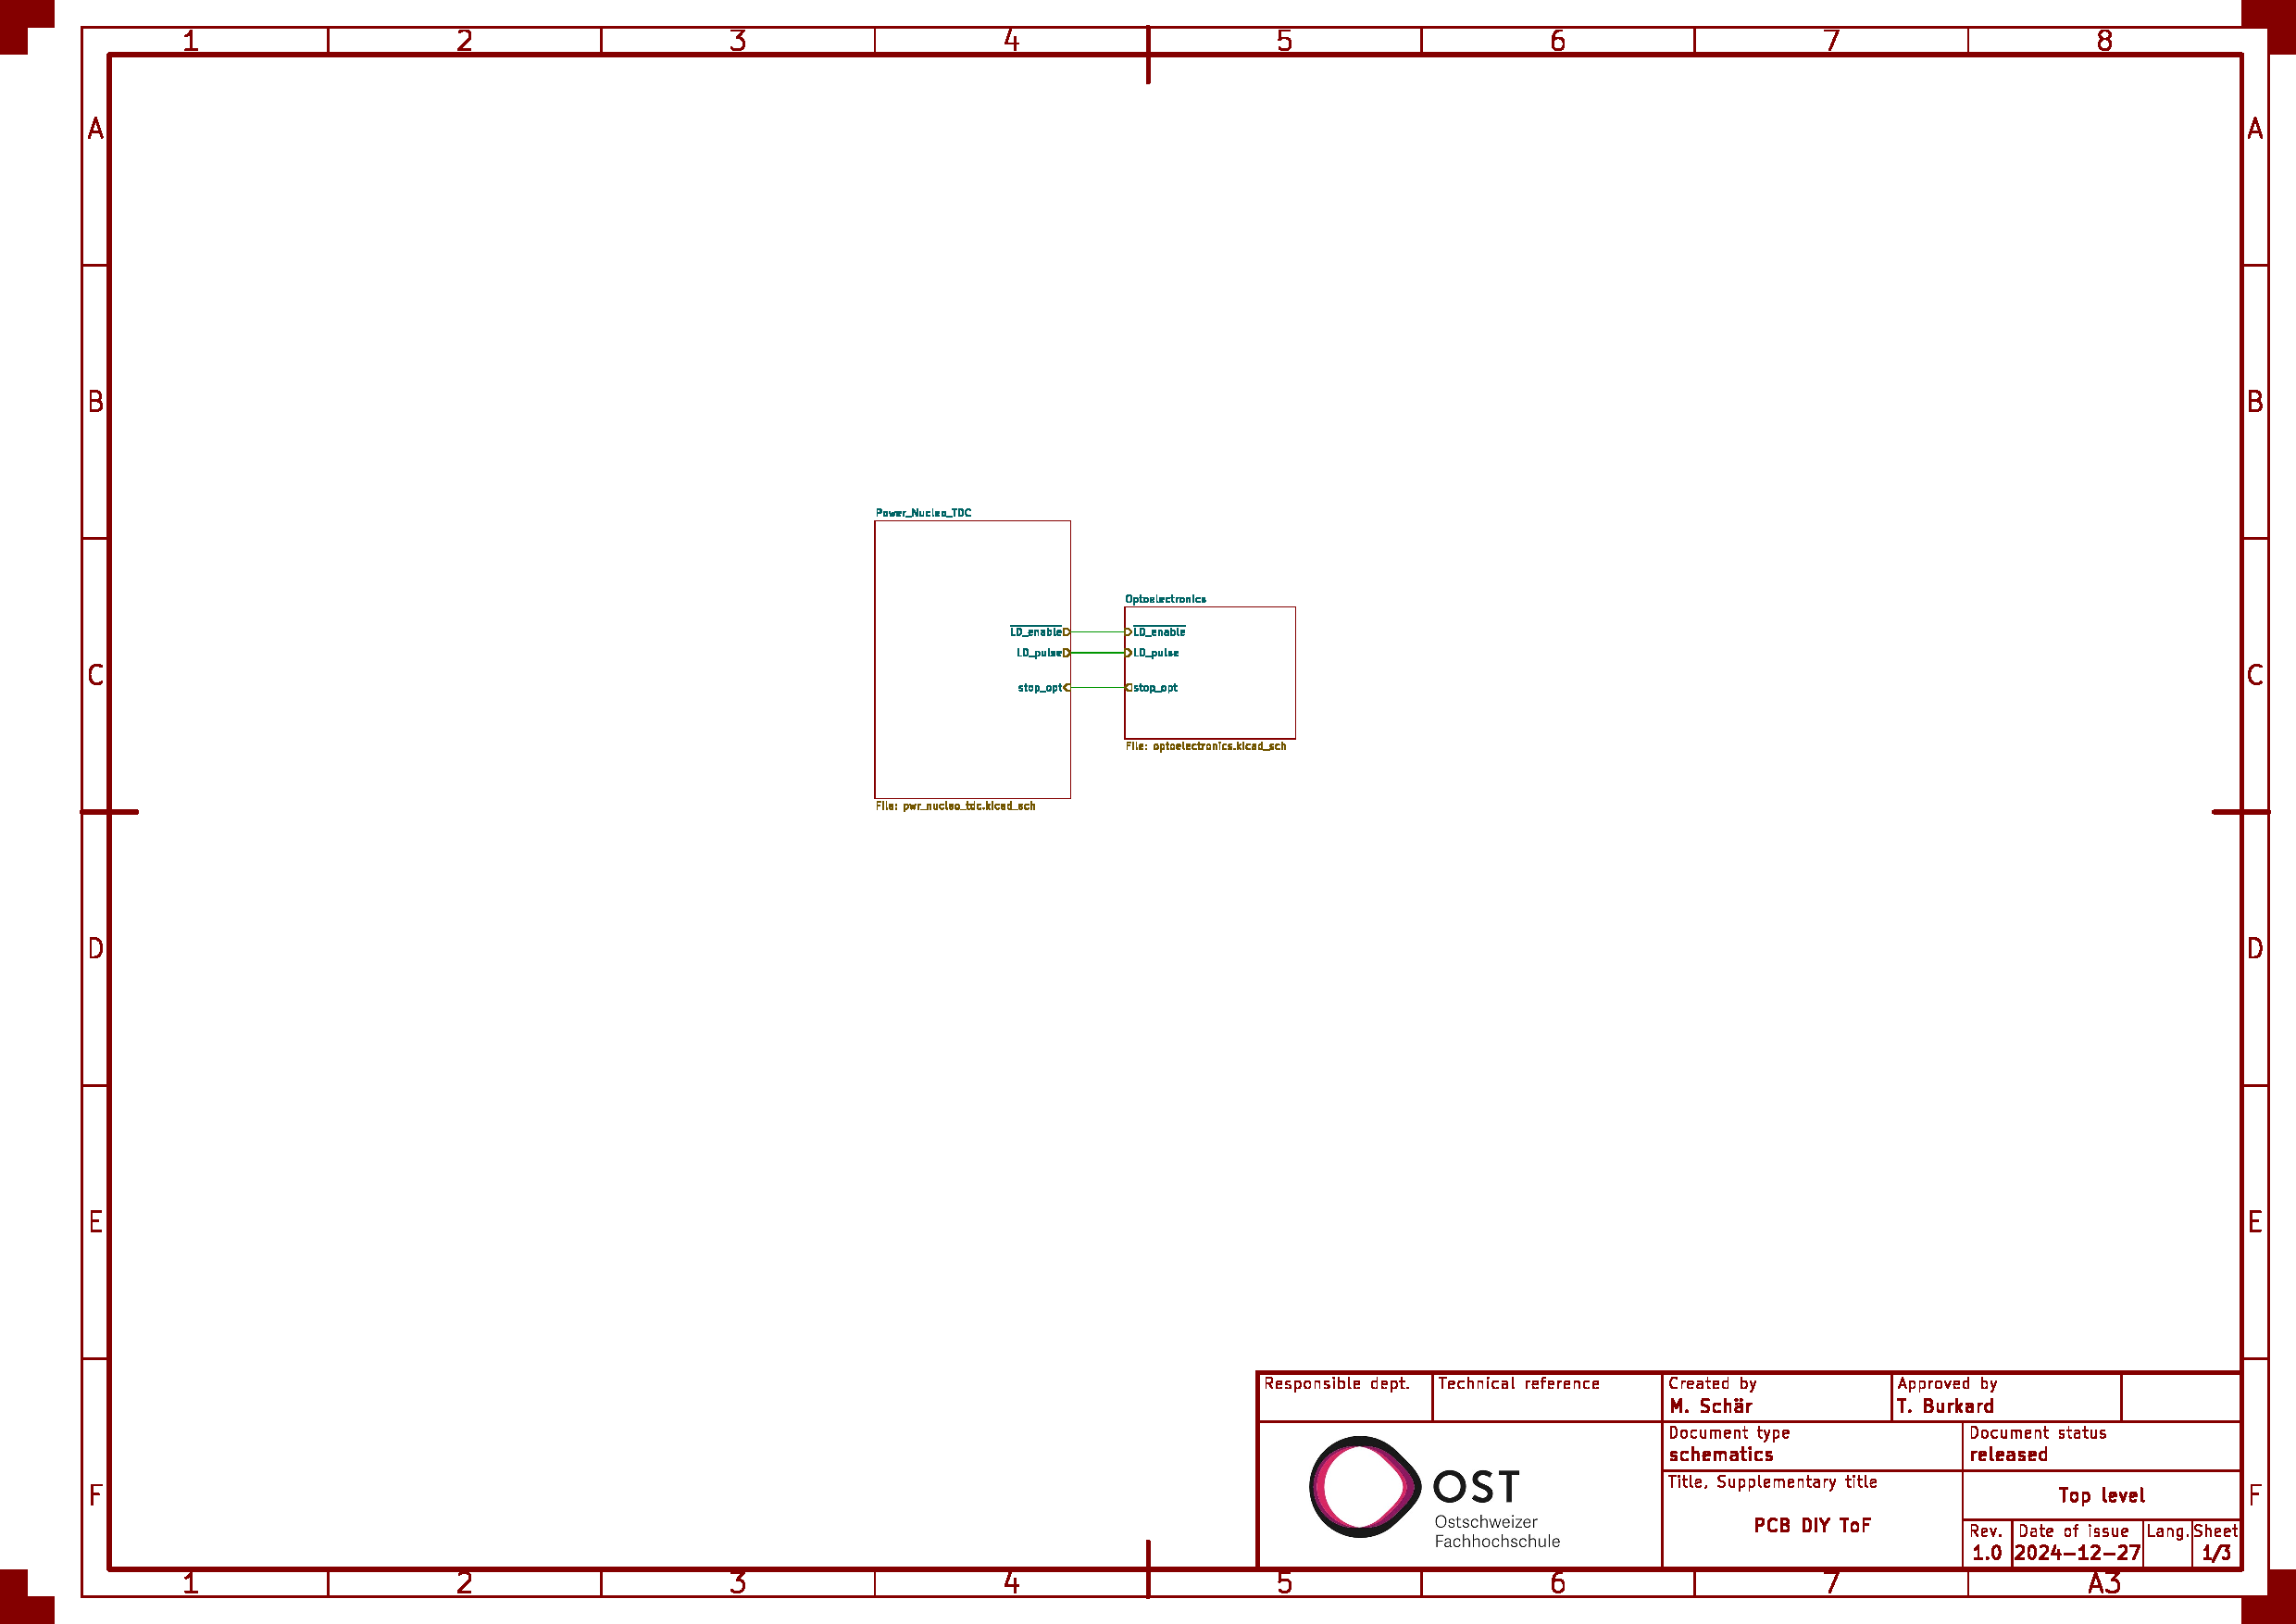
\includegraphics[page=1, width=1.2\textwidth]{attachments/schematic.pdf}
        \caption{Schema S.1/3}\label{fig:schematics_1}
    \end{figure}
    \pagebreak

    \global\pdfpageattr\expandafter{\the\pdfpageattr/Rotate 90}
    \begin{figure}[H]
        \centering
        \includegraphics[page=2, width=1.2\textwidth]{attachments/schematic.pdf}
        \caption{Schema S.2/3}\label{fig:schematics_2}
    \end{figure}
    \pagebreak

    \global\pdfpageattr\expandafter{\the\pdfpageattr/Rotate 90}
    \begin{figure}[H]
        \centering
        \includegraphics[page=3, width=1.2\textwidth]{attachments/schematic.pdf}
        \caption{Schema S.3/3}\label{fig:schematics_3}
    \end{figure}
    \pagebreak


    \subsection{Stückliste}

    \begin{table}[H]
        \scriptsize
        \mytable
            {|l|l|l|l|l|l|}
            {\textbf{Reference} & \textbf{Value} & \textbf{Datasheet} & \textbf{Footprint} & \textbf{Qty} & \textbf{DNP}}
            {\Reference & \Value & \Datasheet & \Footprint & \Qty & \DNP}
            {tables/bom.csv}
        \caption{Bill of Material}\label{tab:bom}
    \end{table}

\end{landscape}
\global\pdfpageattr\expandafter{\the\pdfpageattr/Rotate 0}

\subsection{Layout}\label{sec:apdx_layout}

\begin{figure}[H]
    \centering
    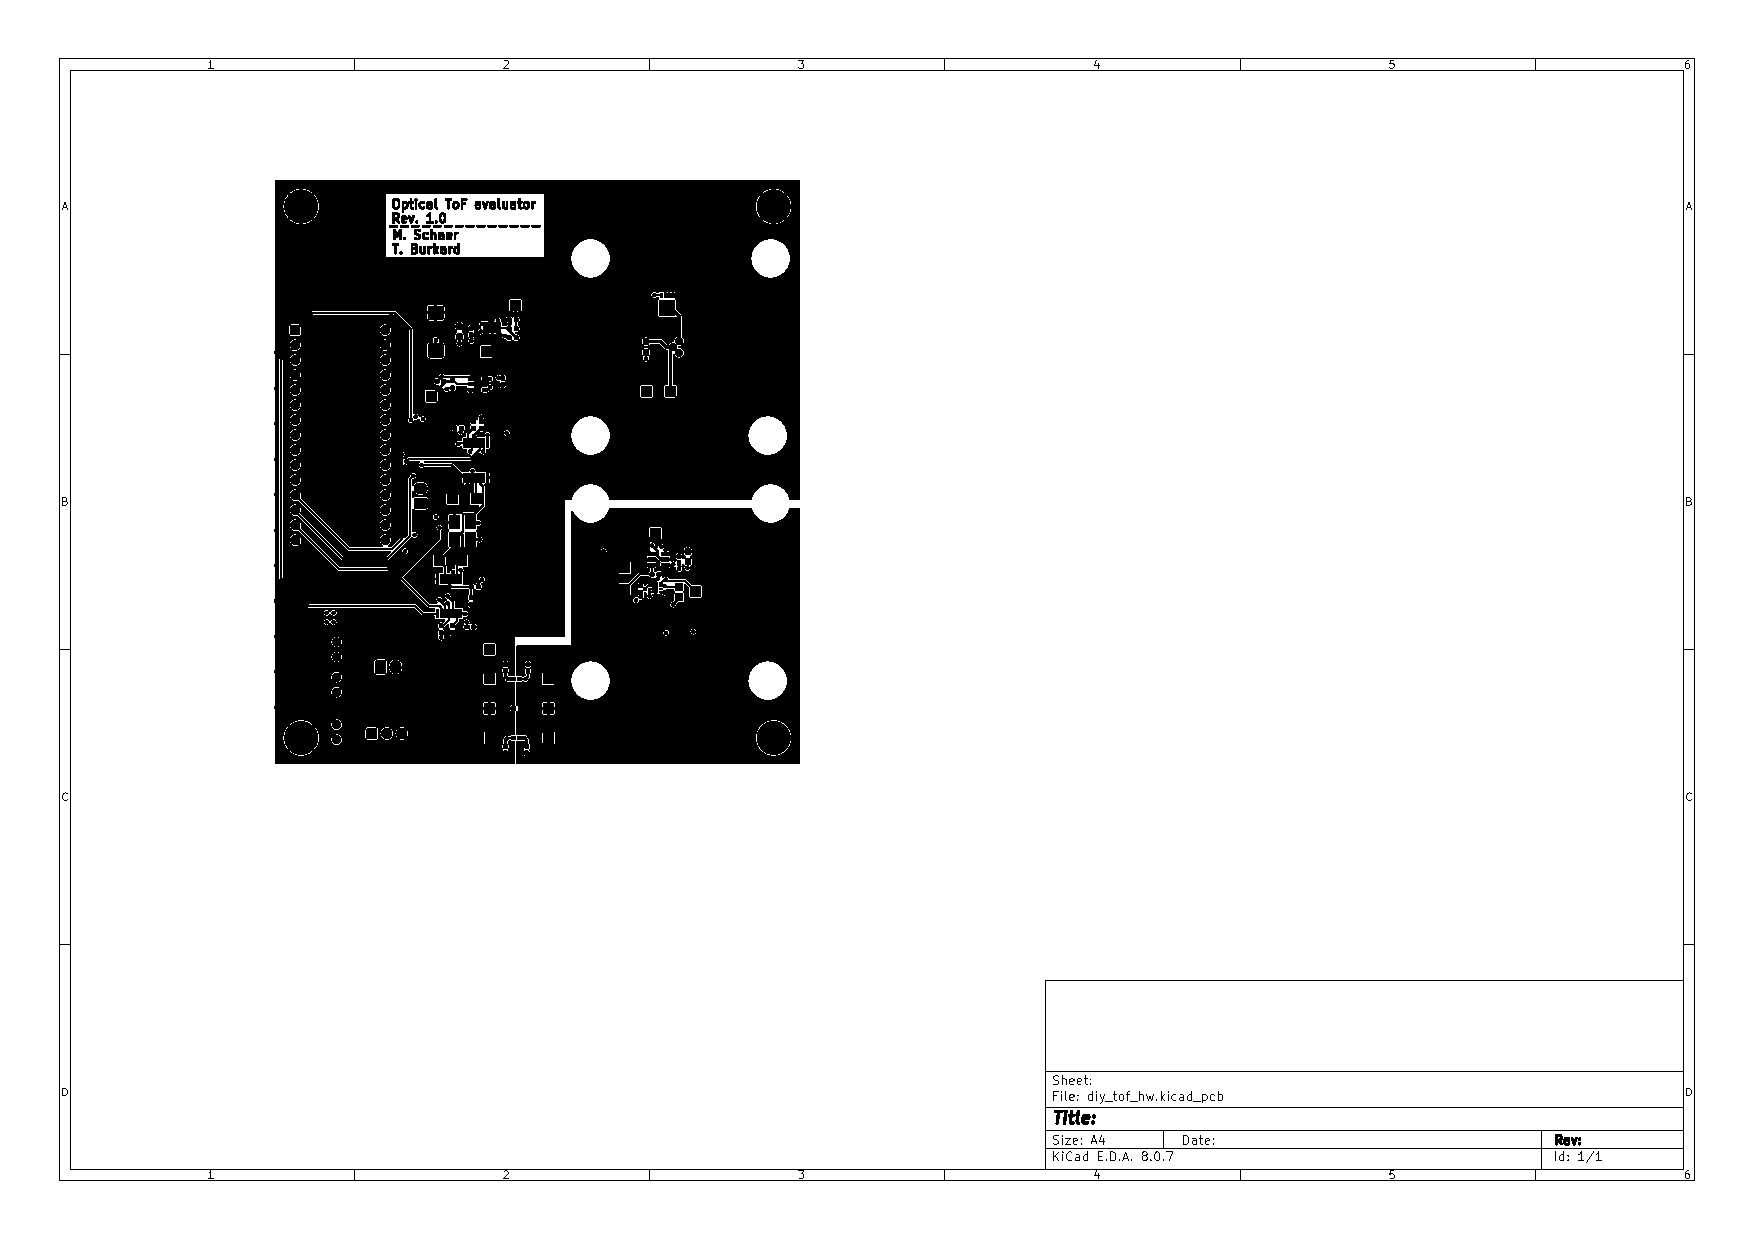
\includegraphics[trim=130 220 450 80, clip, width=0.6\textwidth]{attachments/pcb_F_Cu.pdf}
    \caption{PCB Layout Top}\label{fig:apdx_pcb_f_cu}
\end{figure}

\begin{figure}[H]
    \centering
    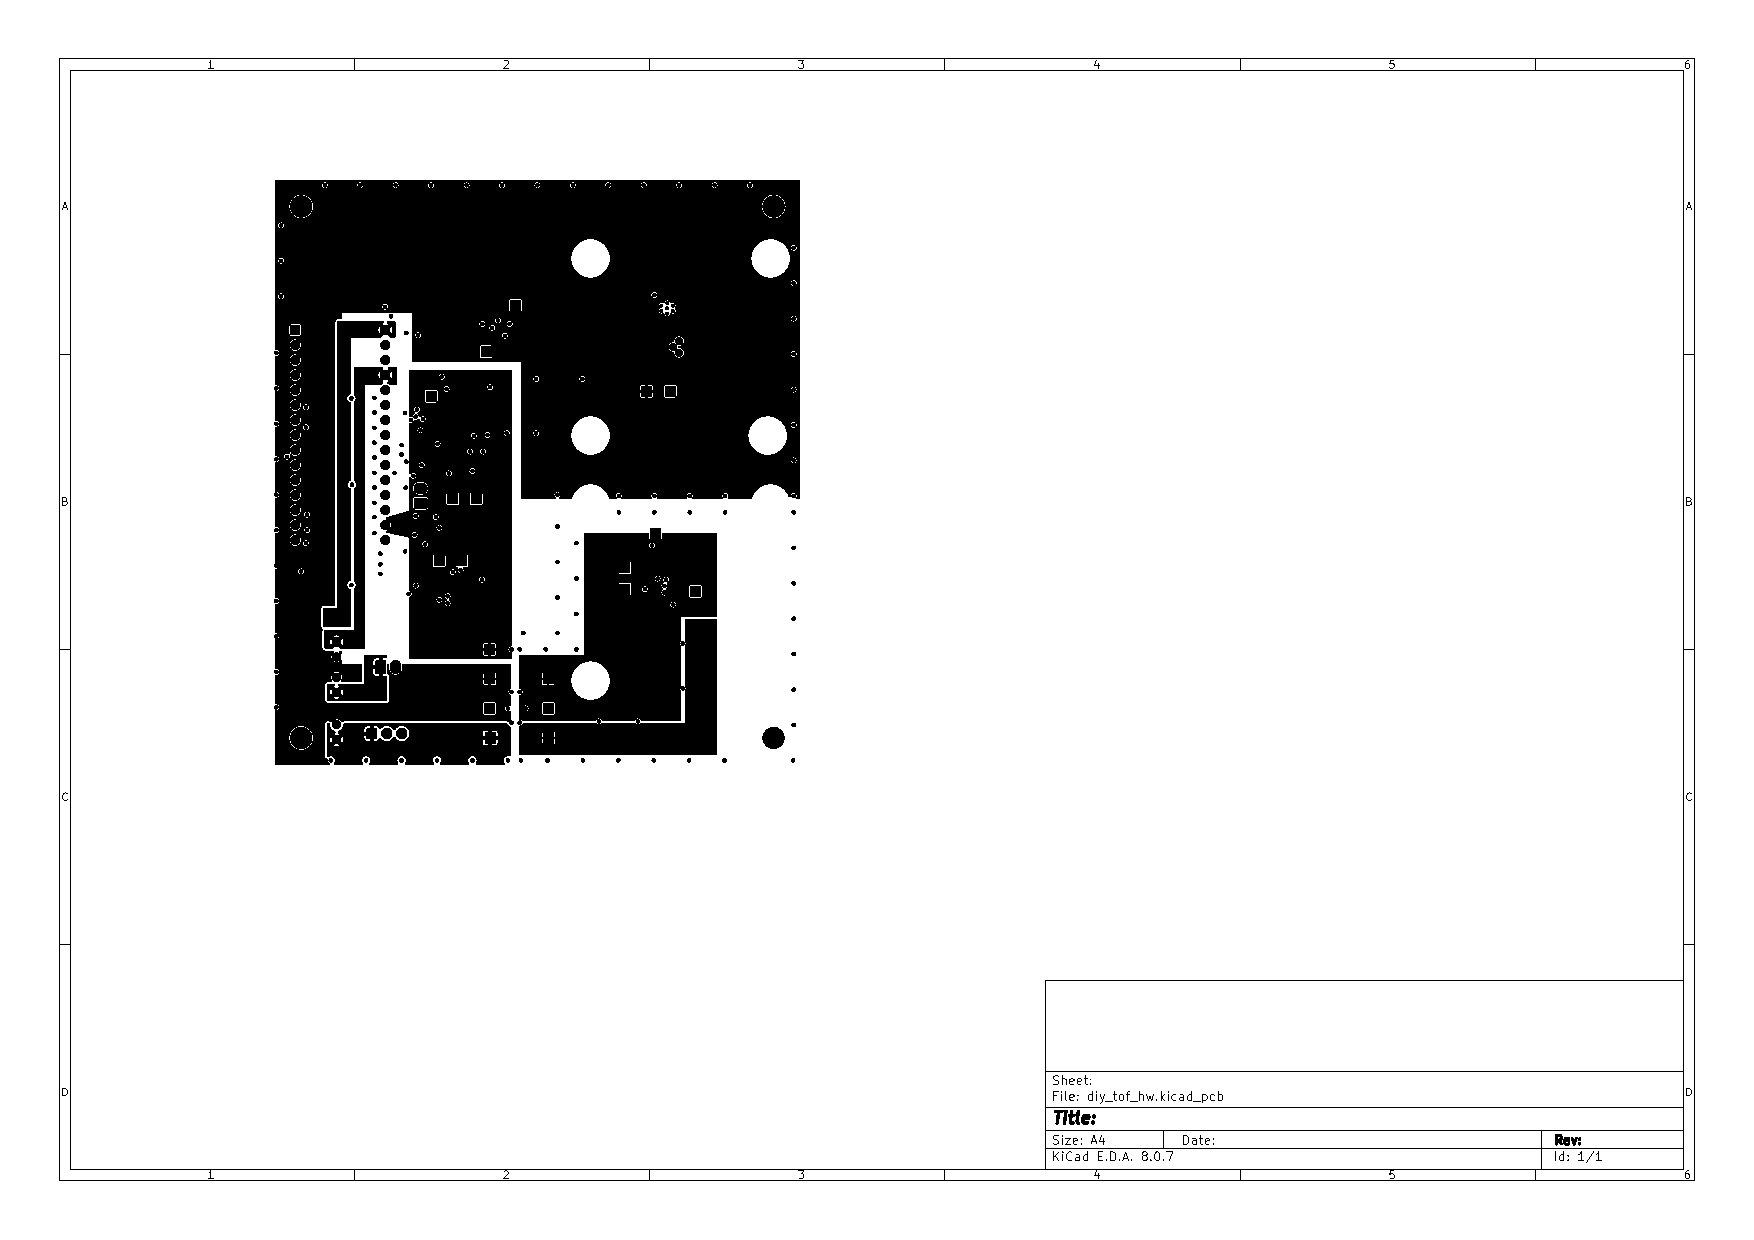
\includegraphics[trim=130 220 450 80, clip, width=0.6\textwidth]{attachments/pcb_In1_Cu.pdf}
    \caption{PCB Layout Innen 1}\label{fig:apdx_pcb_in1_cu}
\end{figure}

\begin{figure}[H]
    \centering
    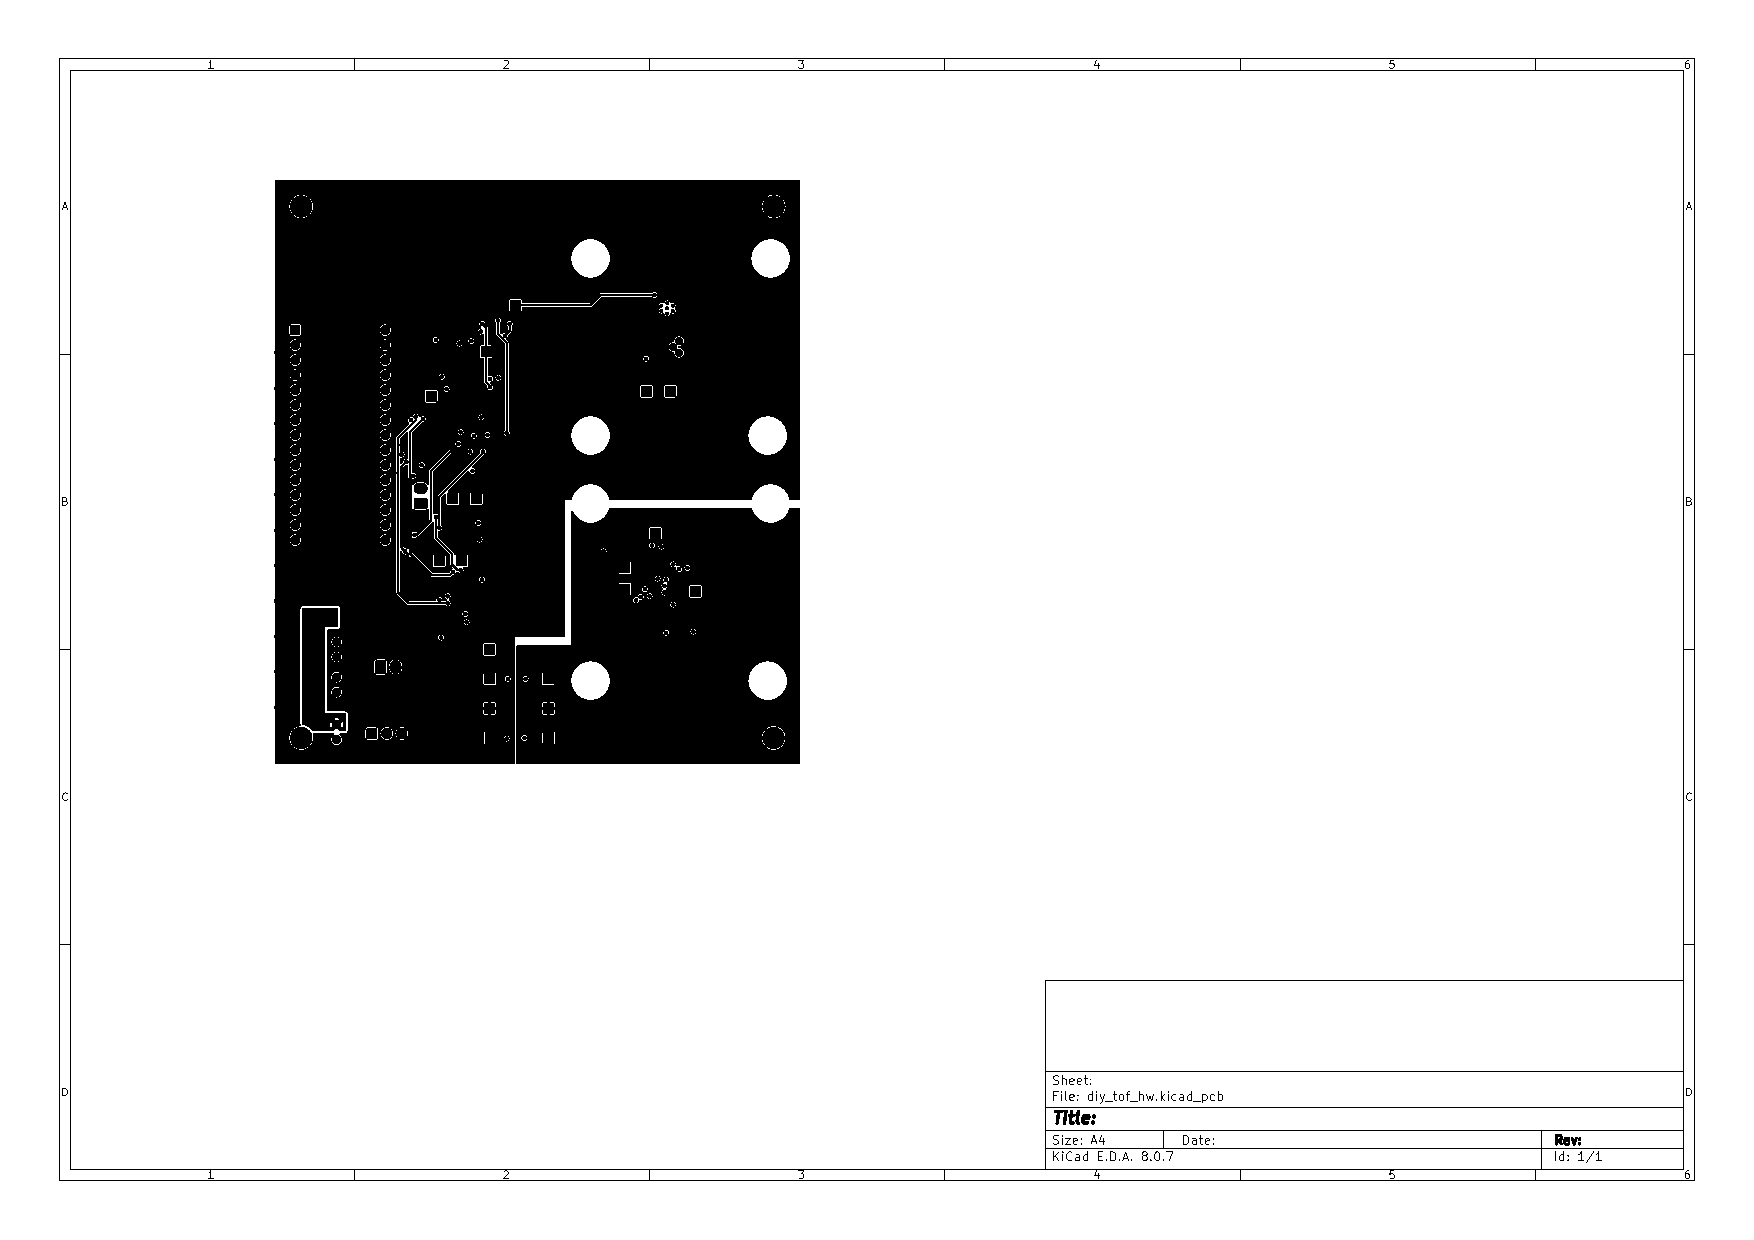
\includegraphics[trim=130 220 450 80, clip, width=0.6\textwidth]{attachments/pcb_In2_Cu.pdf}
    \caption{PCB Layout Innen 2}\label{fig:apdx_pcb_in2_cu}
\end{figure}

\begin{figure}[H]
    \centering
    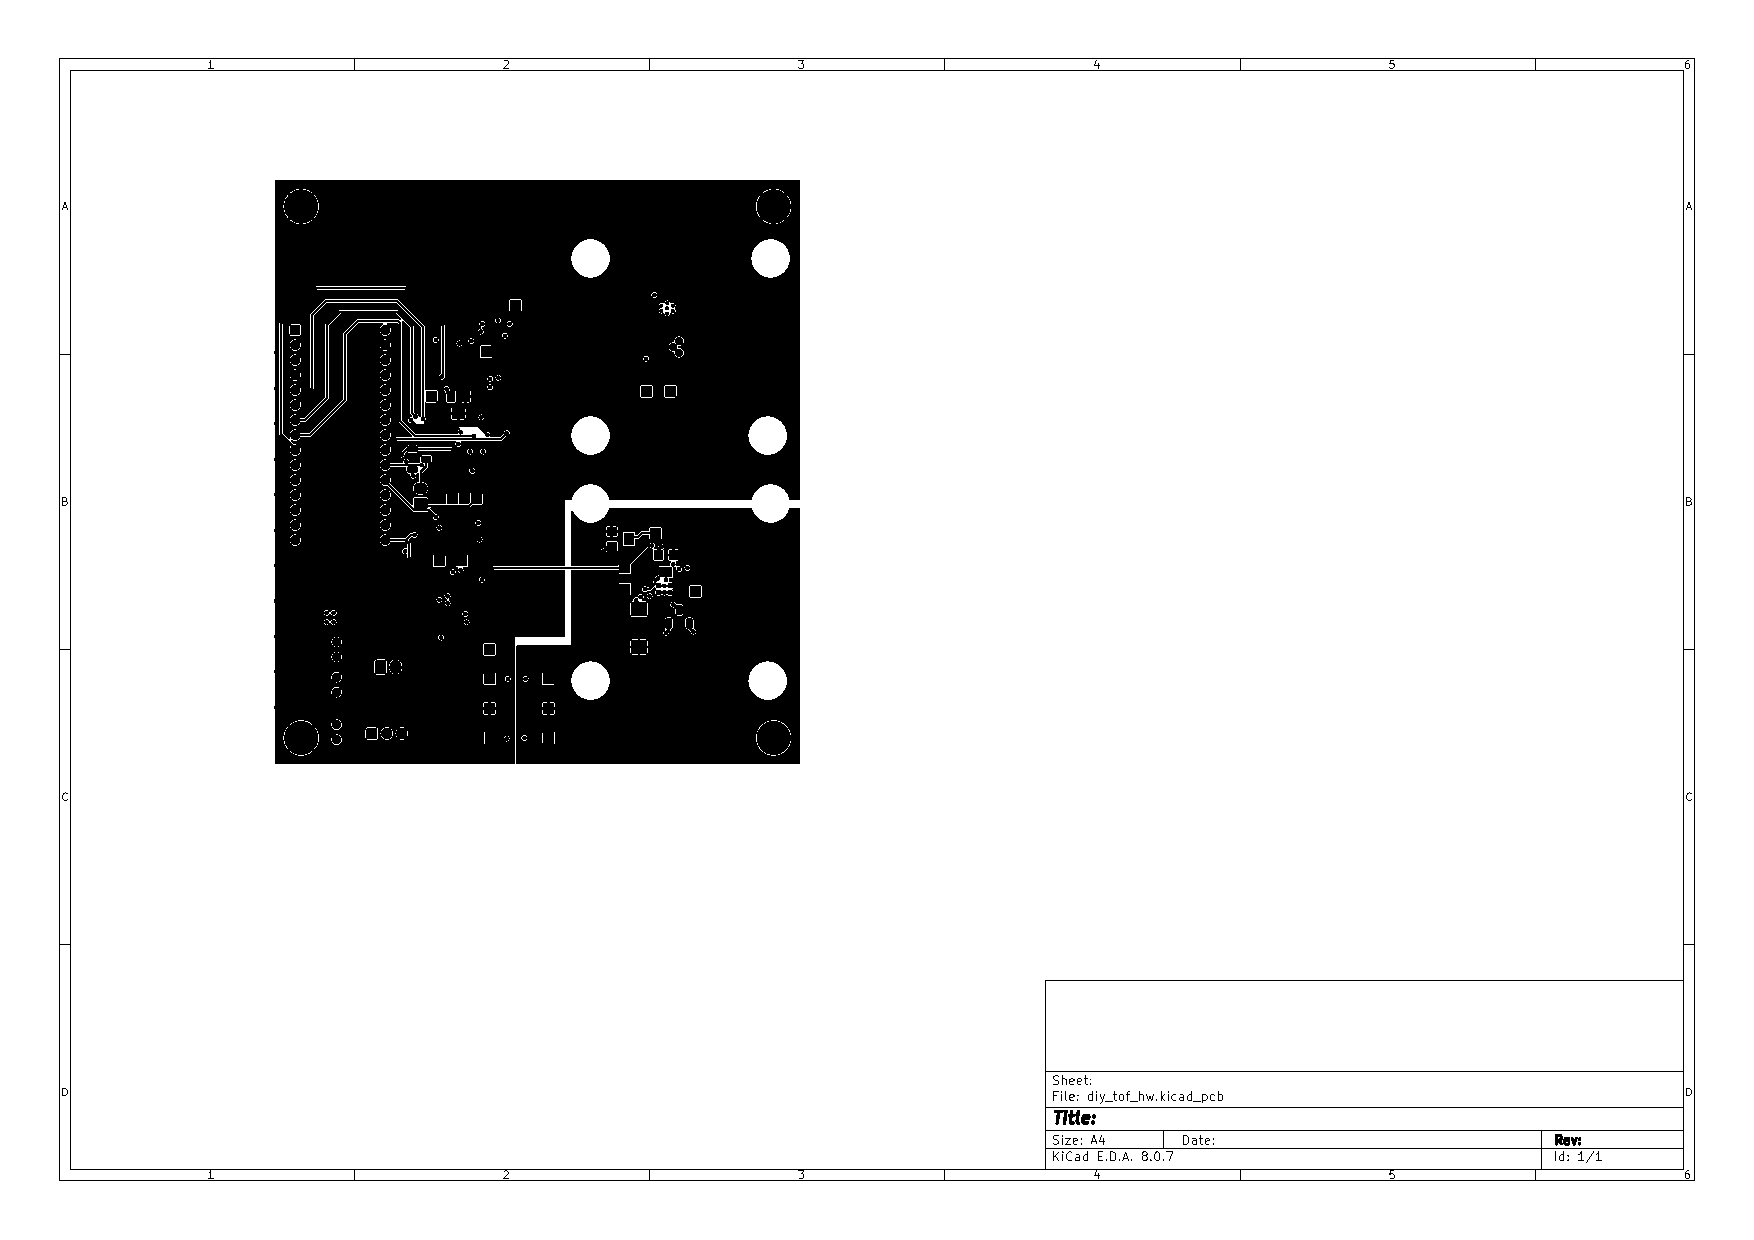
\includegraphics[trim=130 220 450 80, clip, width=0.6\textwidth]{attachments/pcb_B_Cu.pdf}
    \caption{PCB Layout Bottom}\label{fig:apdx_pcb_b_cu}
\end{figure}

\subsection{Komponenten-Platzierung}\label{sec:apdx_placement}

\begin{figure}[H]
    \centering
    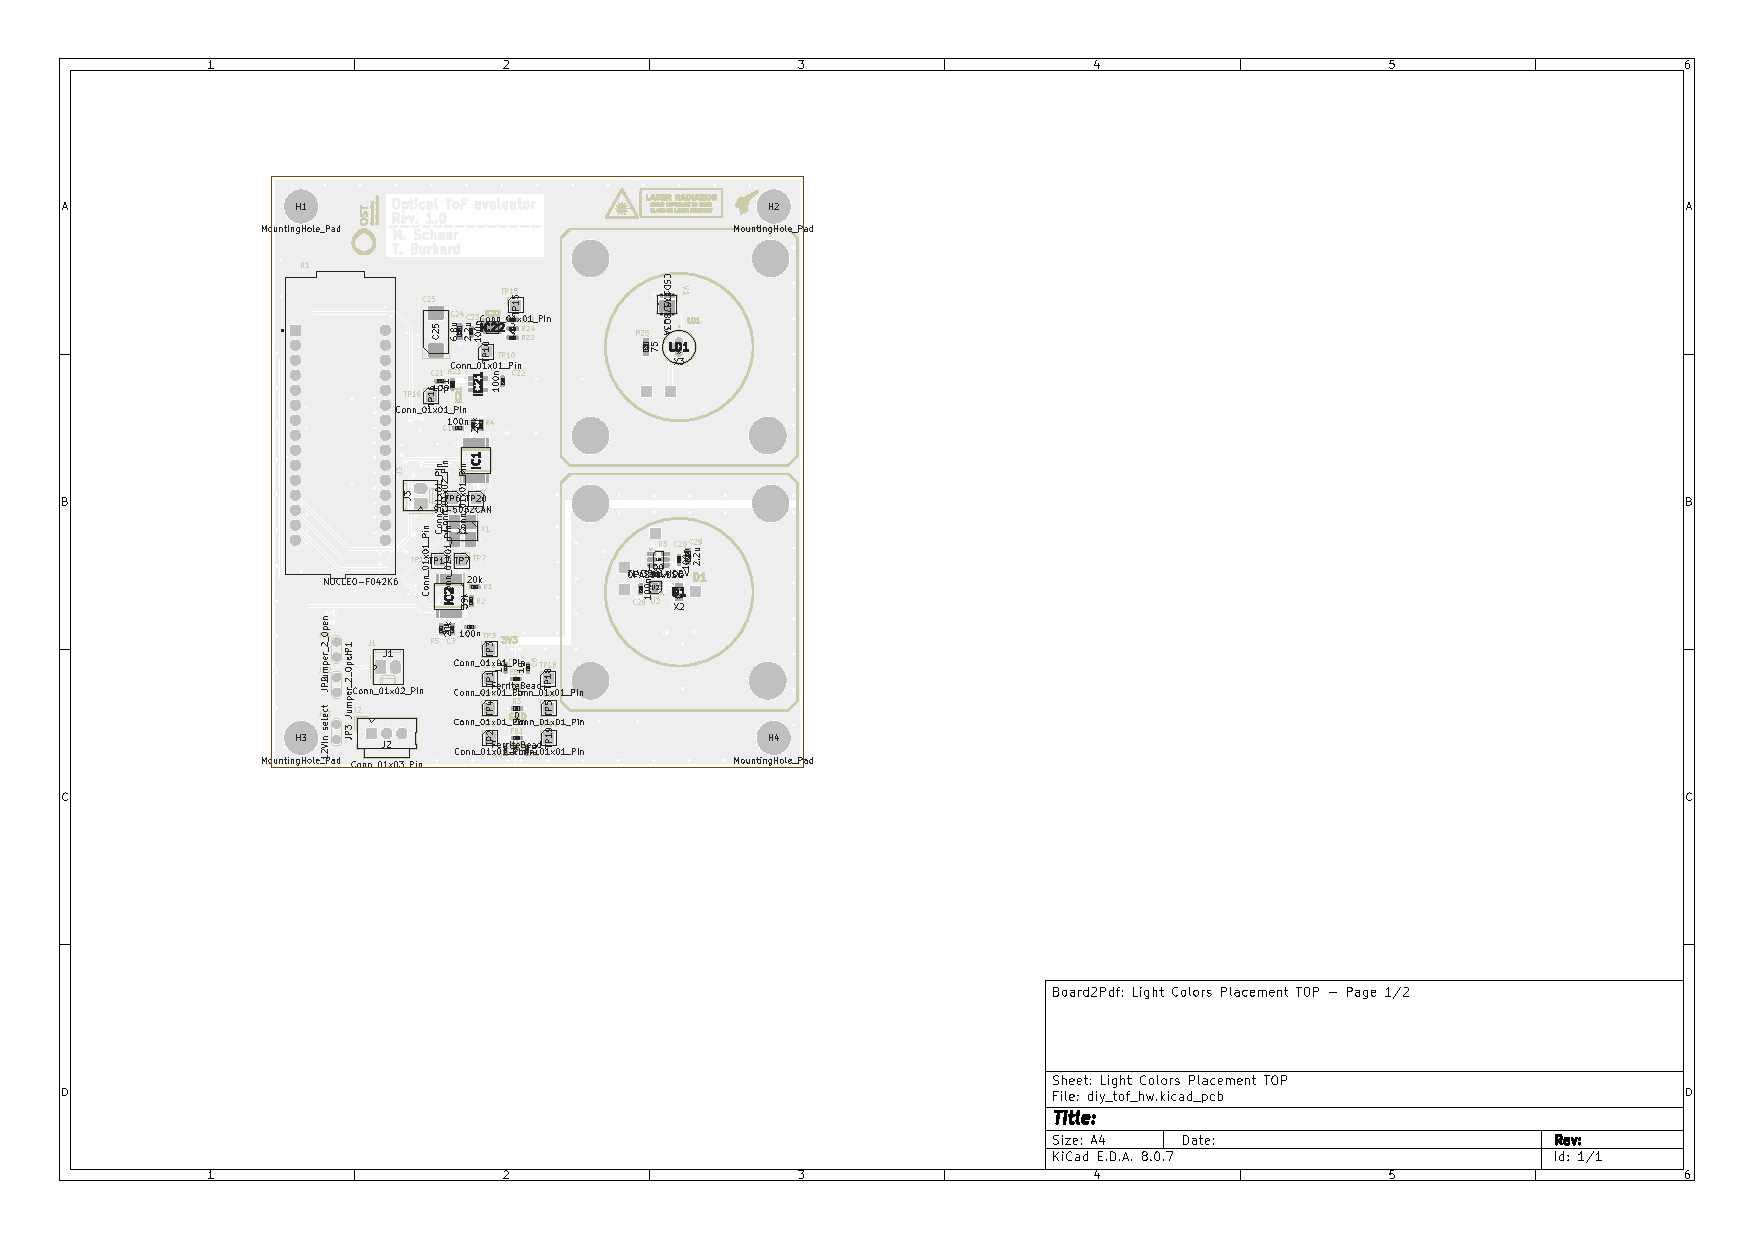
\includegraphics[page=1, trim=120 220 450 80, clip, width=0.6\textwidth]{attachments/pcb_placement.pdf}
    \caption{PCB Komponenten-Platzierung Top}\label{fig:apdx_pcb_placement_1}
\end{figure}

\begin{figure}[H]
    \centering
    \includegraphics[page=2, trim=450 220 120 80, clip, width=0.6\textwidth]{attachments/pcb_placement.pdf}
    \caption{PCB Komponenten-Platzierung Bottom}\label{fig:apdx_pcb_placement_2}
\end{figure}
\pagebreak

\subsection{3D View}\label{sec:apdx_3D_view}

\begin{figure}[H]
    \centering
    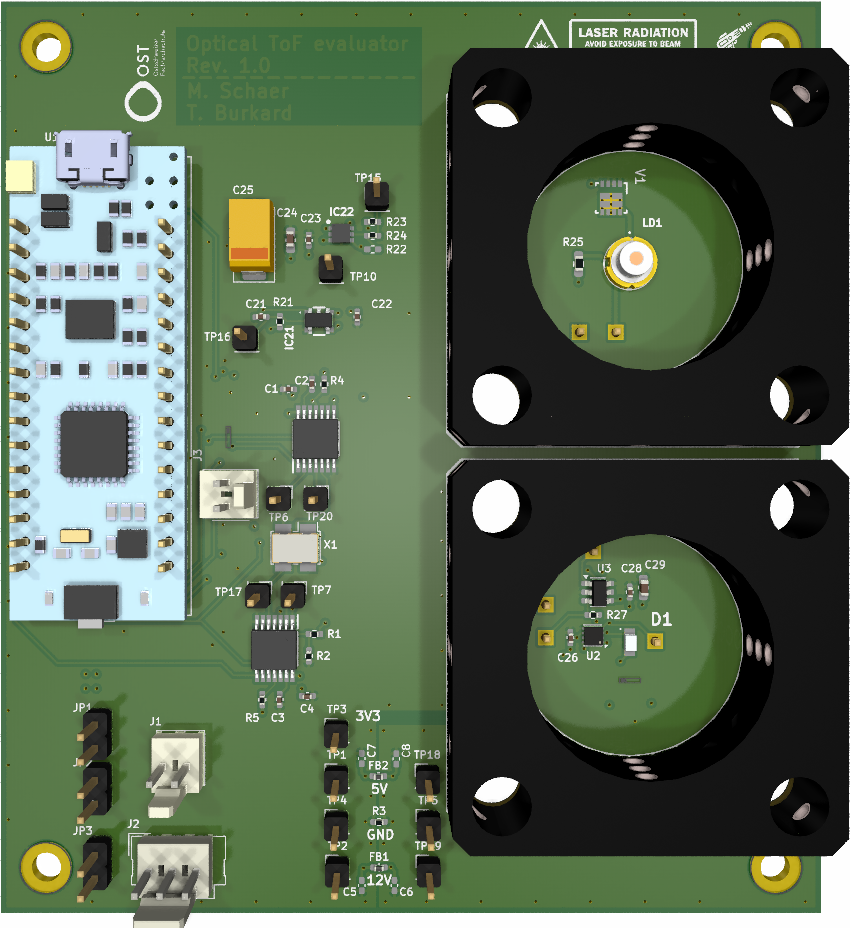
\includegraphics[width=0.5\textwidth]{graphics/3d_top.png}
    \caption{3D View Top}\label{fig:apdx_3d_top}
\end{figure}

\begin{figure}[H]
    \centering
    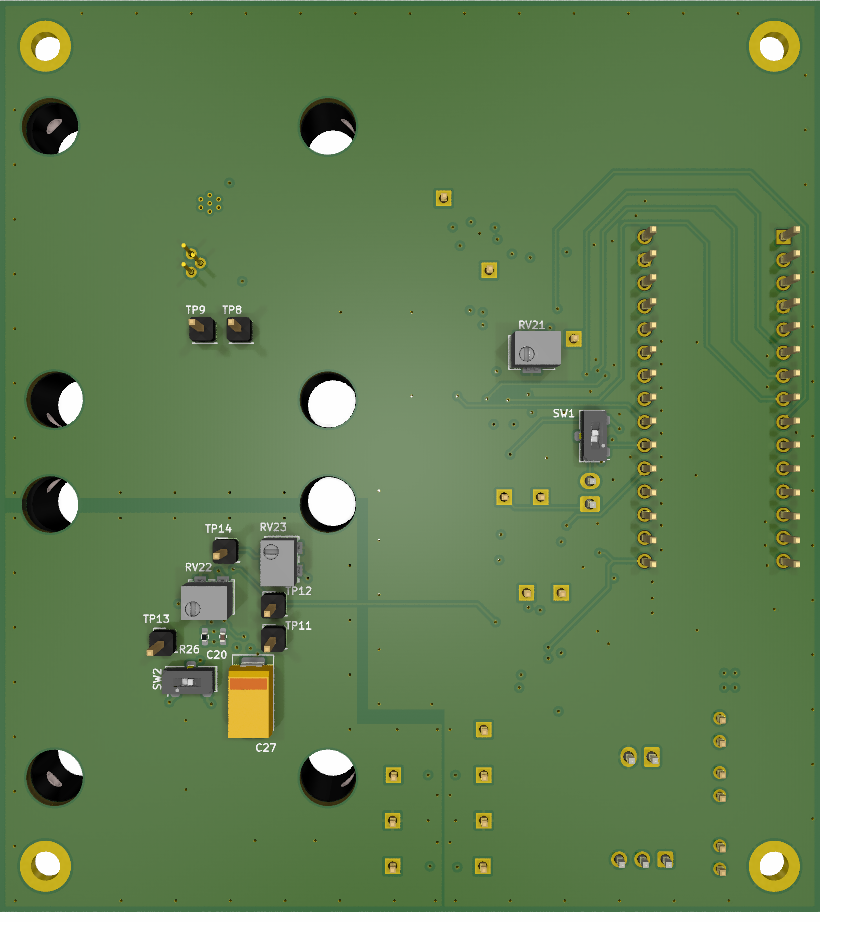
\includegraphics[width=0.5\textwidth]{graphics/3d_bottom.png}
    \caption{3D View Bottom}\label{fig:apdx_3d_bottom}
\end{figure}

\subsection{Fotos Demonstrator}\label{sec:apdx_photos_demonstrator}

\begin{figure}[H]
    \centering
    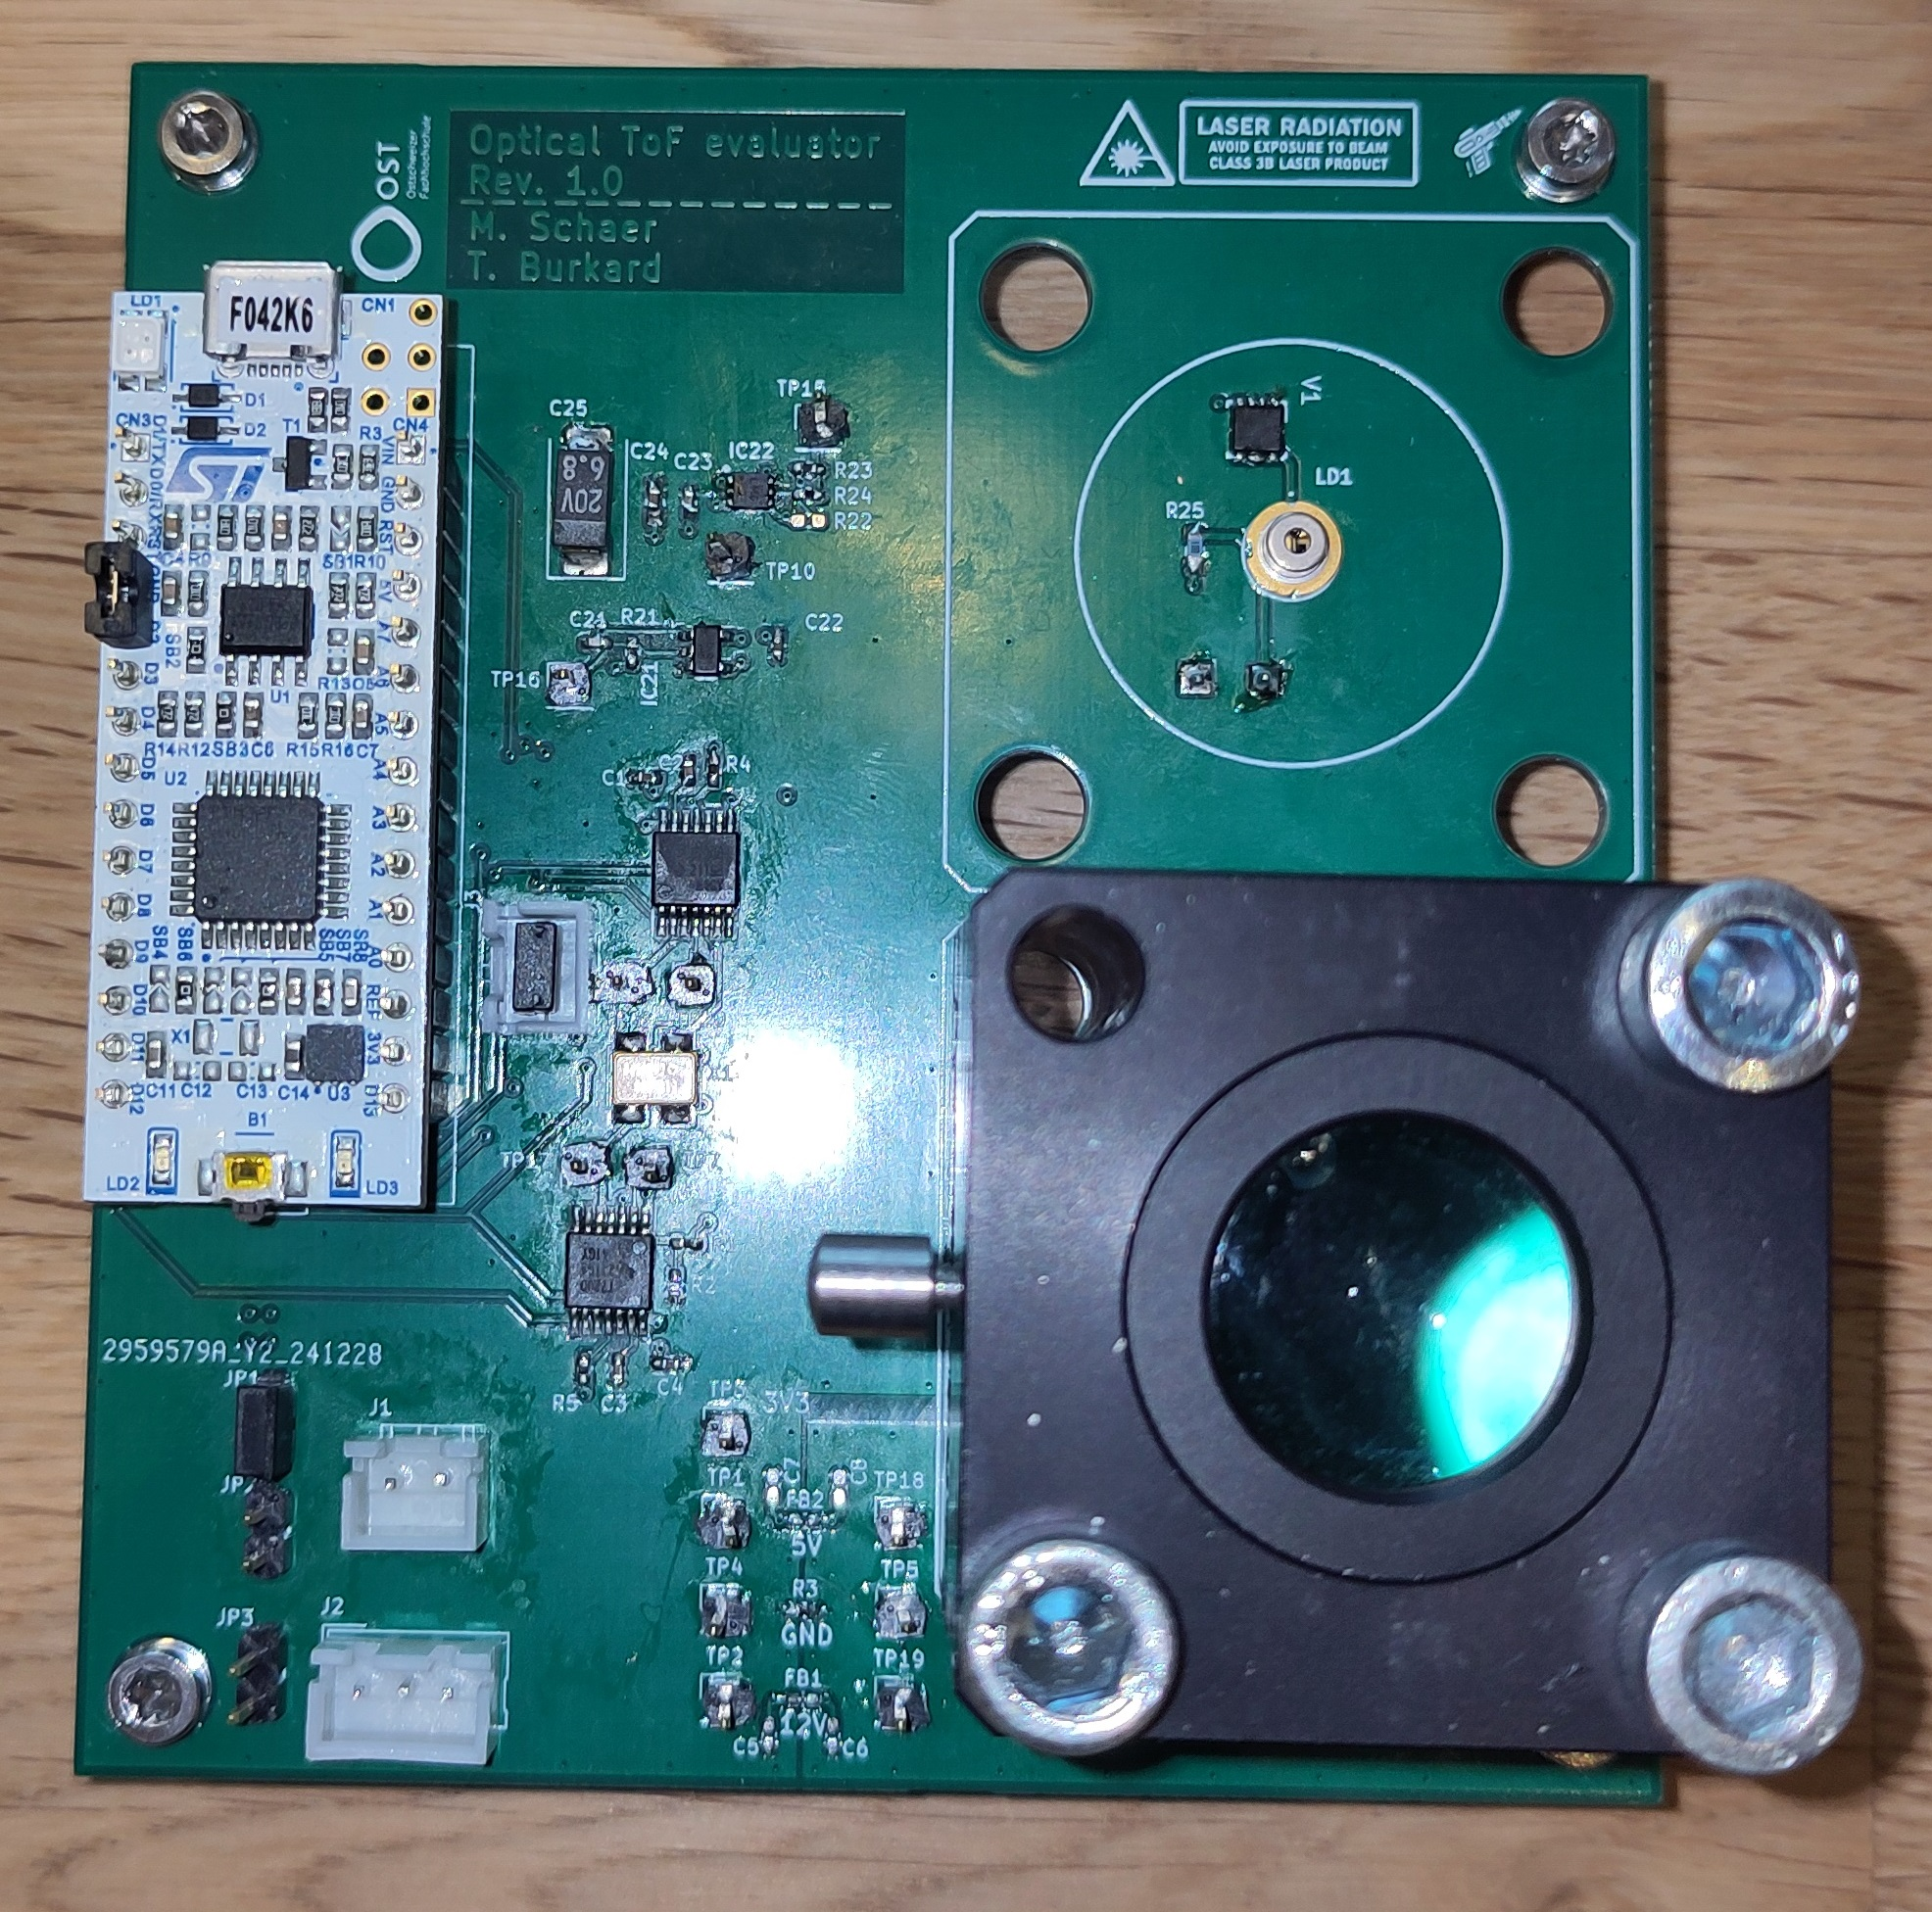
\includegraphics[width=0.6\textwidth]{graphics/photo_demonstrator_top.jpg}
    \caption{Demonstrator von oben}\label{fig:apdx_photo_demonstrator_top}
\end{figure}

\begin{figure}[H]
    \centering
    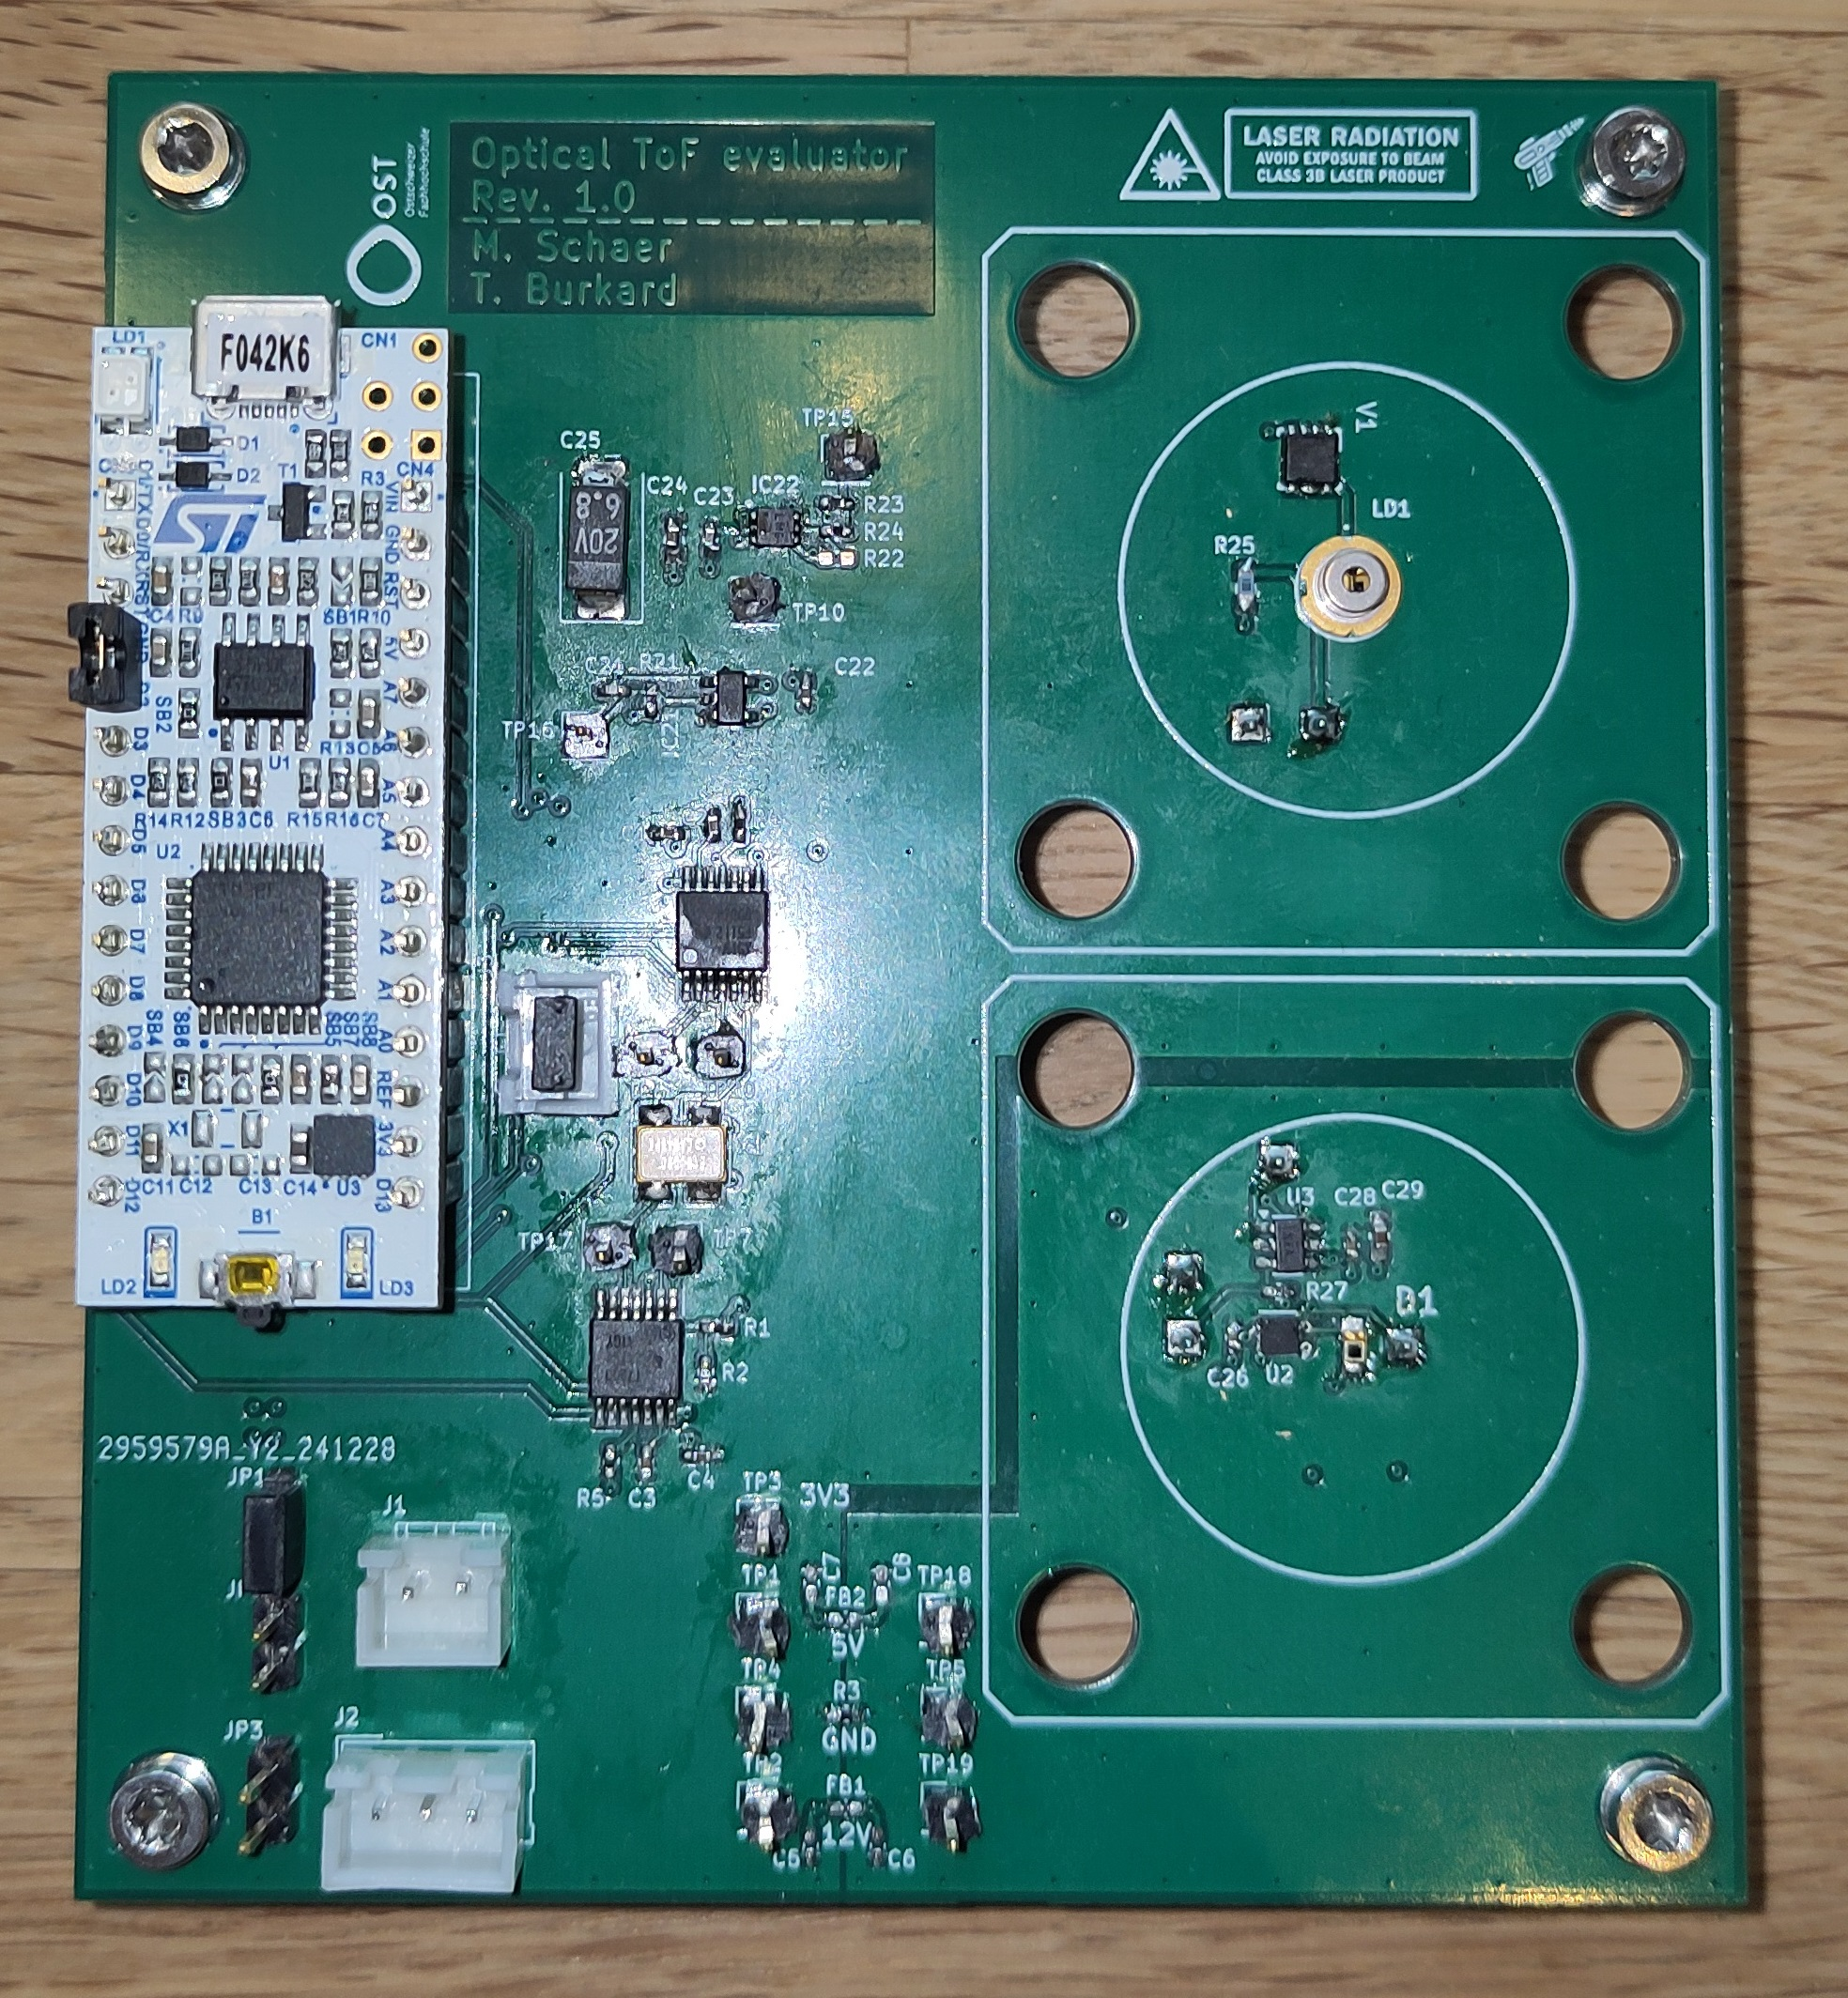
\includegraphics[width=0.6\textwidth]{graphics/photo_demonstrator_top_wo_lens.jpg}
    \caption{Demonstrator von oben ohne Linse}\label{fig:apdx_photo_demonstrator_top_wo_lens}
\end{figure}

\begin{figure}[H]
    \centering
    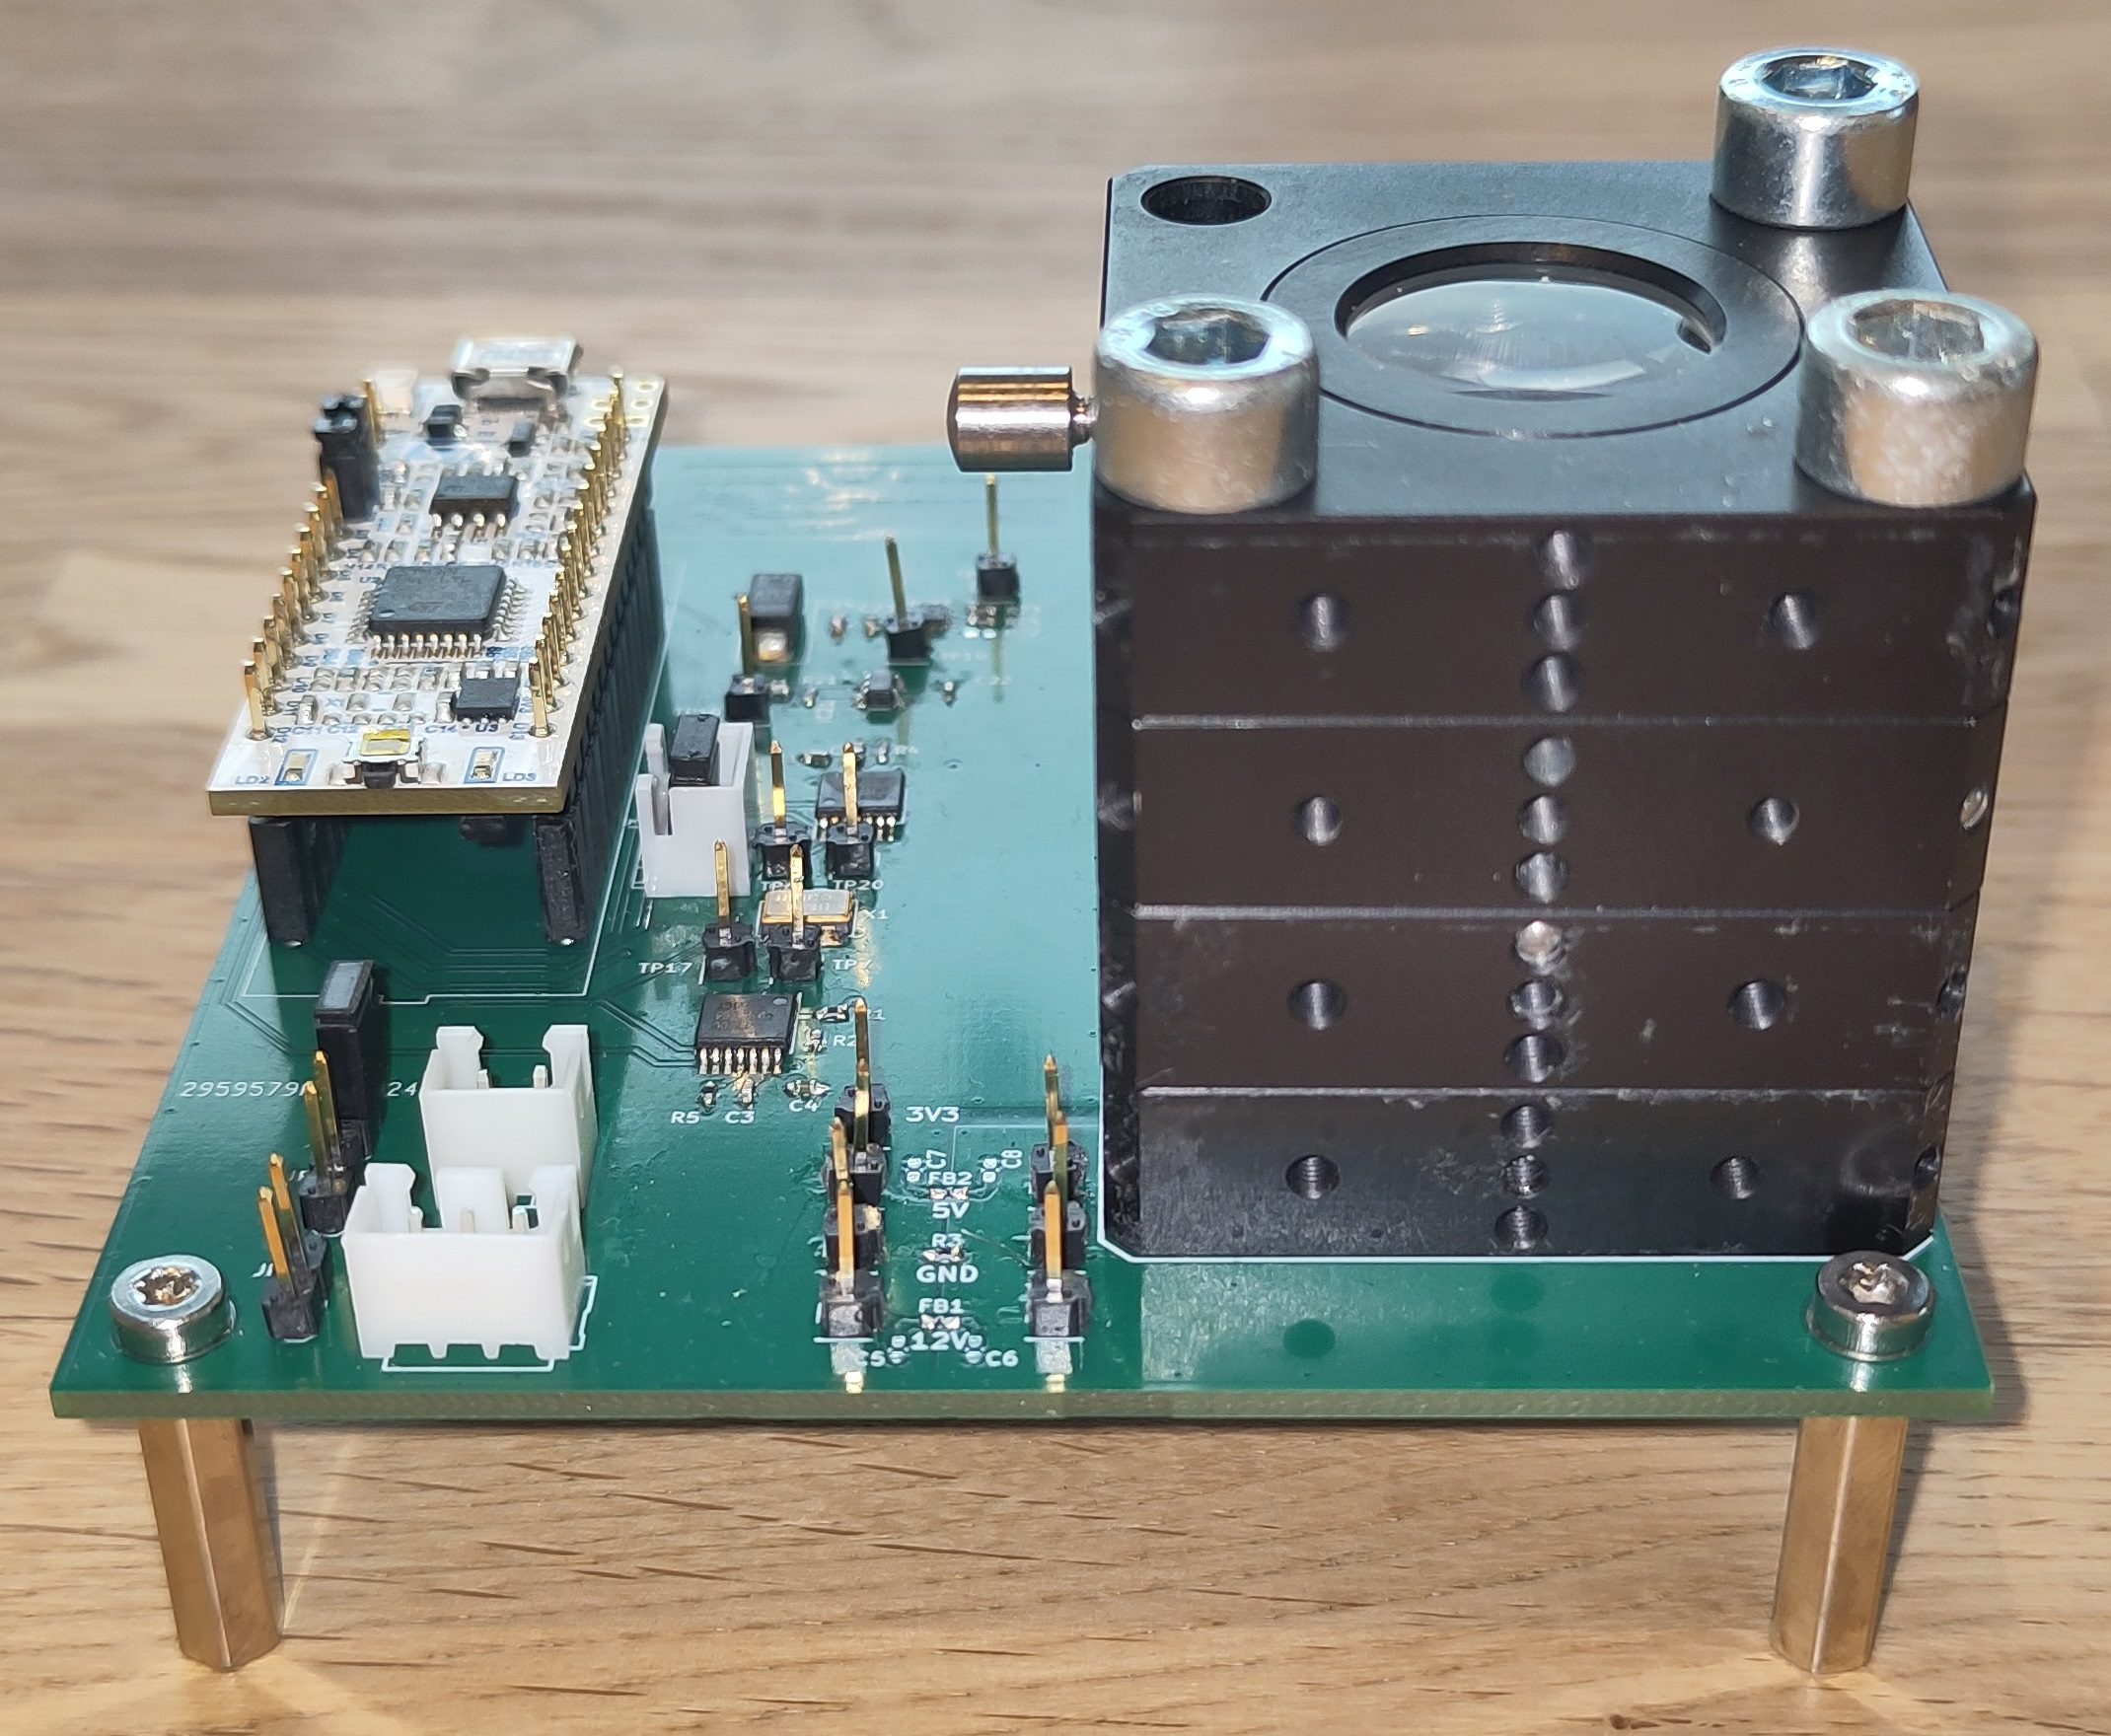
\includegraphics[width=0.6\textwidth]{graphics/photo_demonstrator_front.jpg}
    \caption{Demonstrator von vorne}\label{fig:apdx_photo_demonstrator_front}
\end{figure}

\begin{figure}[H]
    \centering
    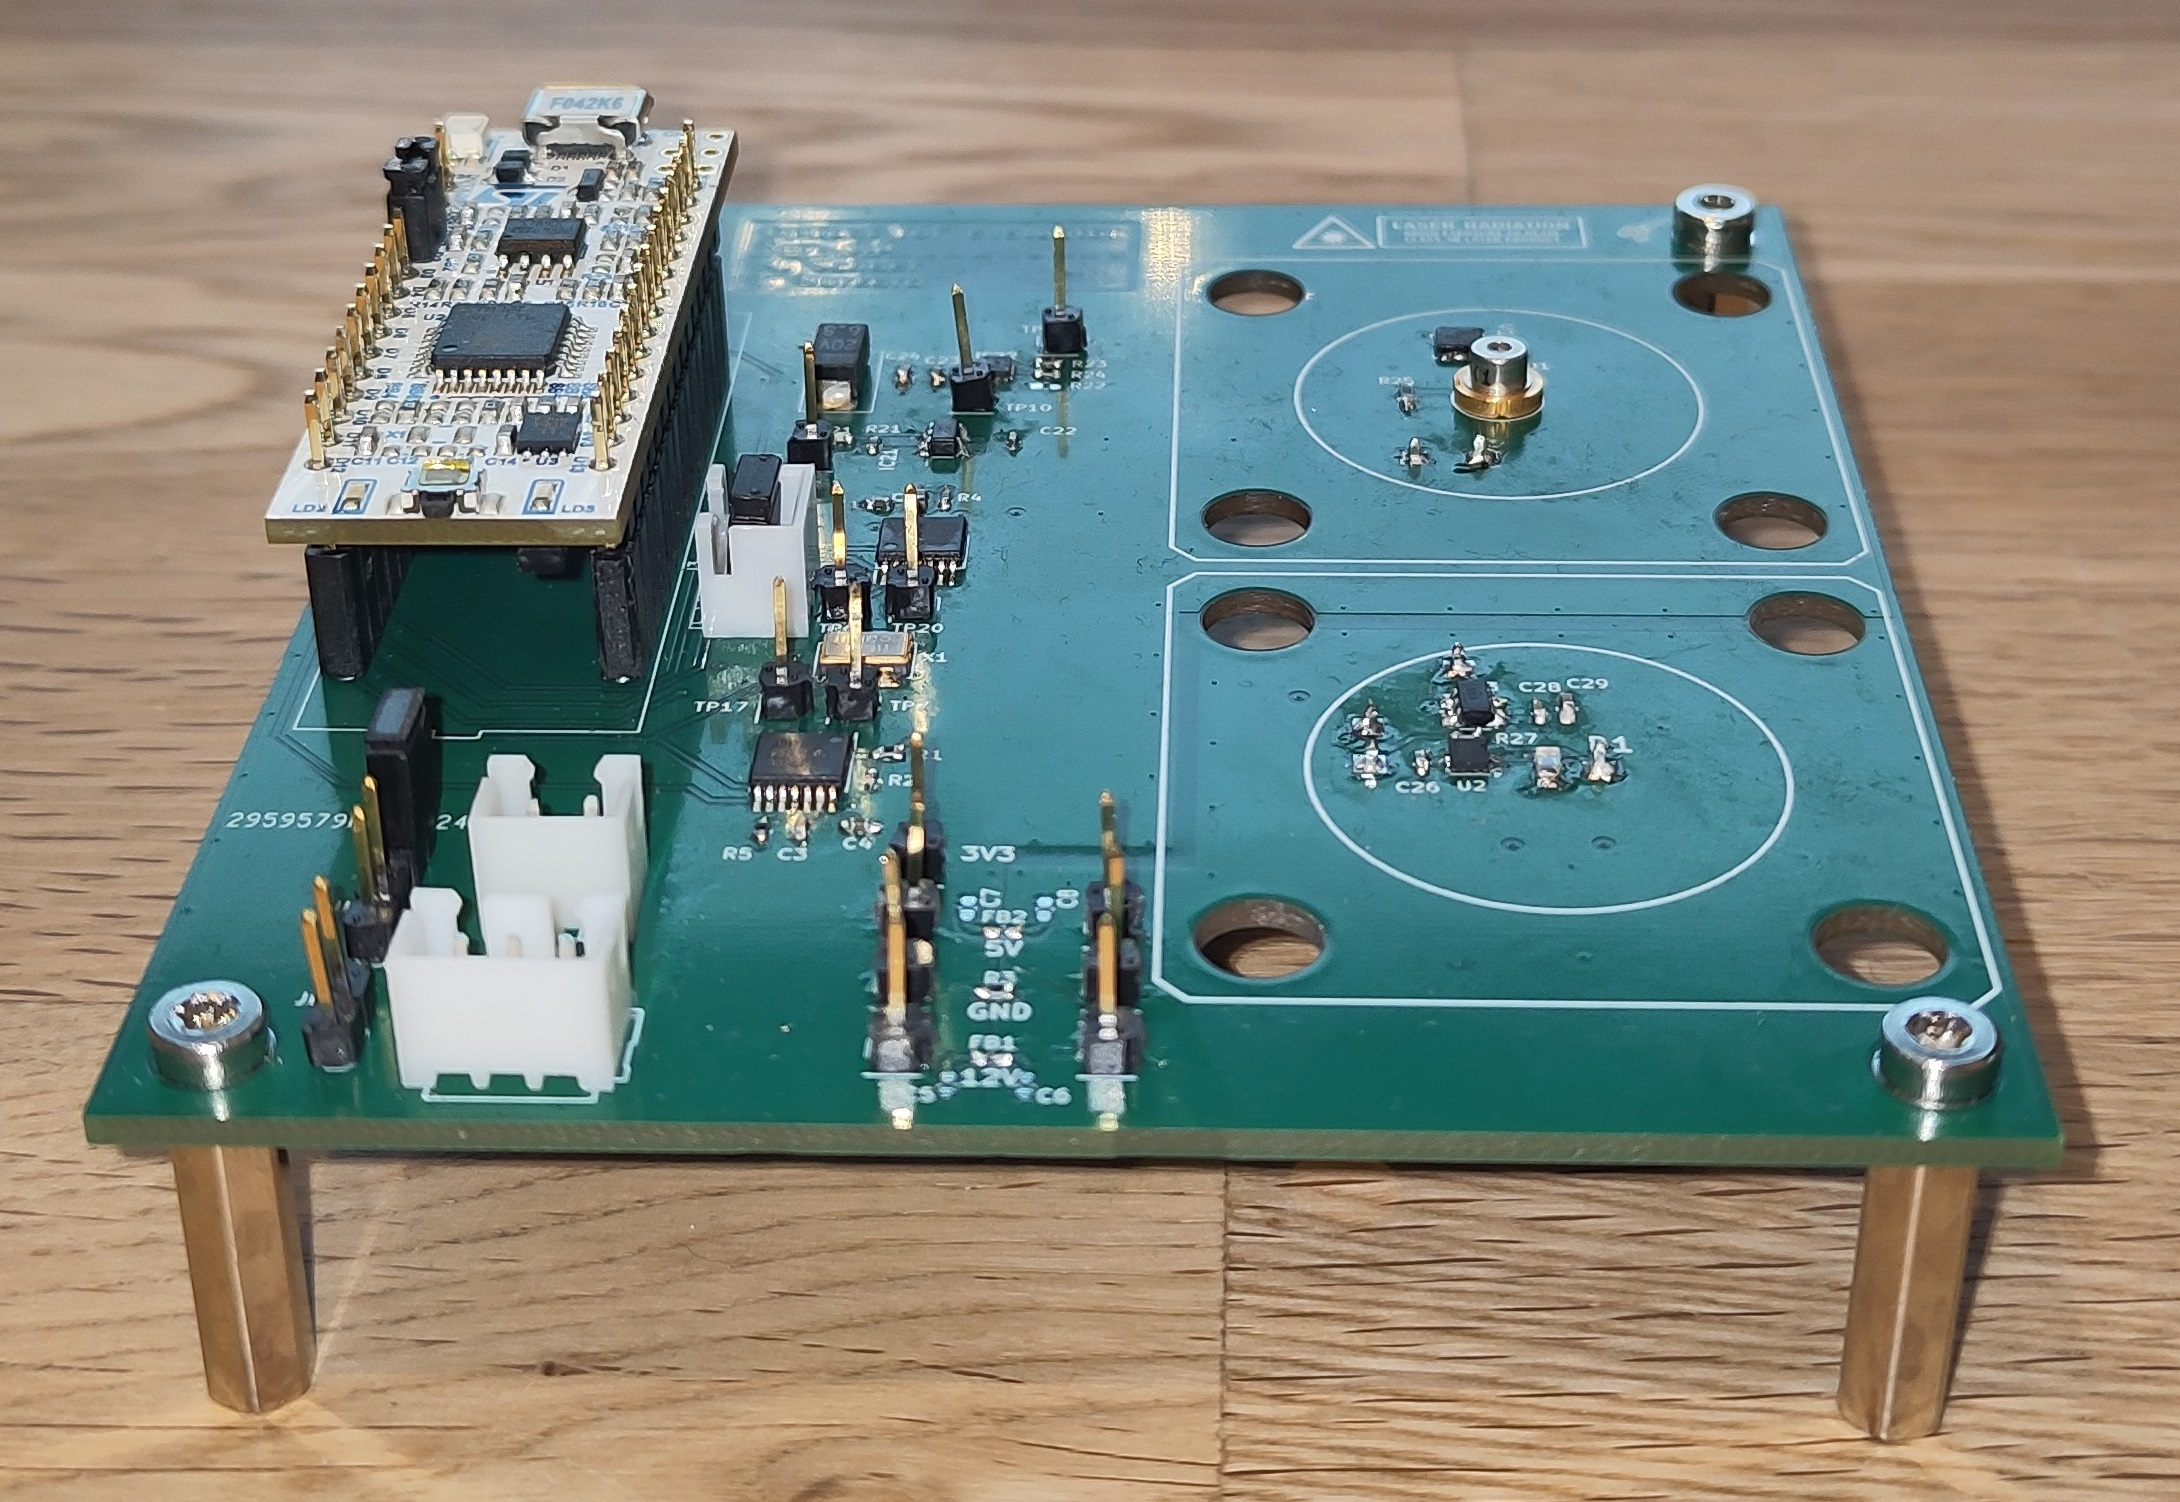
\includegraphics[width=0.6\textwidth]{graphics/photo_demonstrator_front_wo_lens.jpg}
    \caption{Demonstrator von vorne ohne Linse}\label{fig:apdx_photo_demonstrator_front_wo_lens}
\end{figure}

\begin{figure}[H]
    \centering
    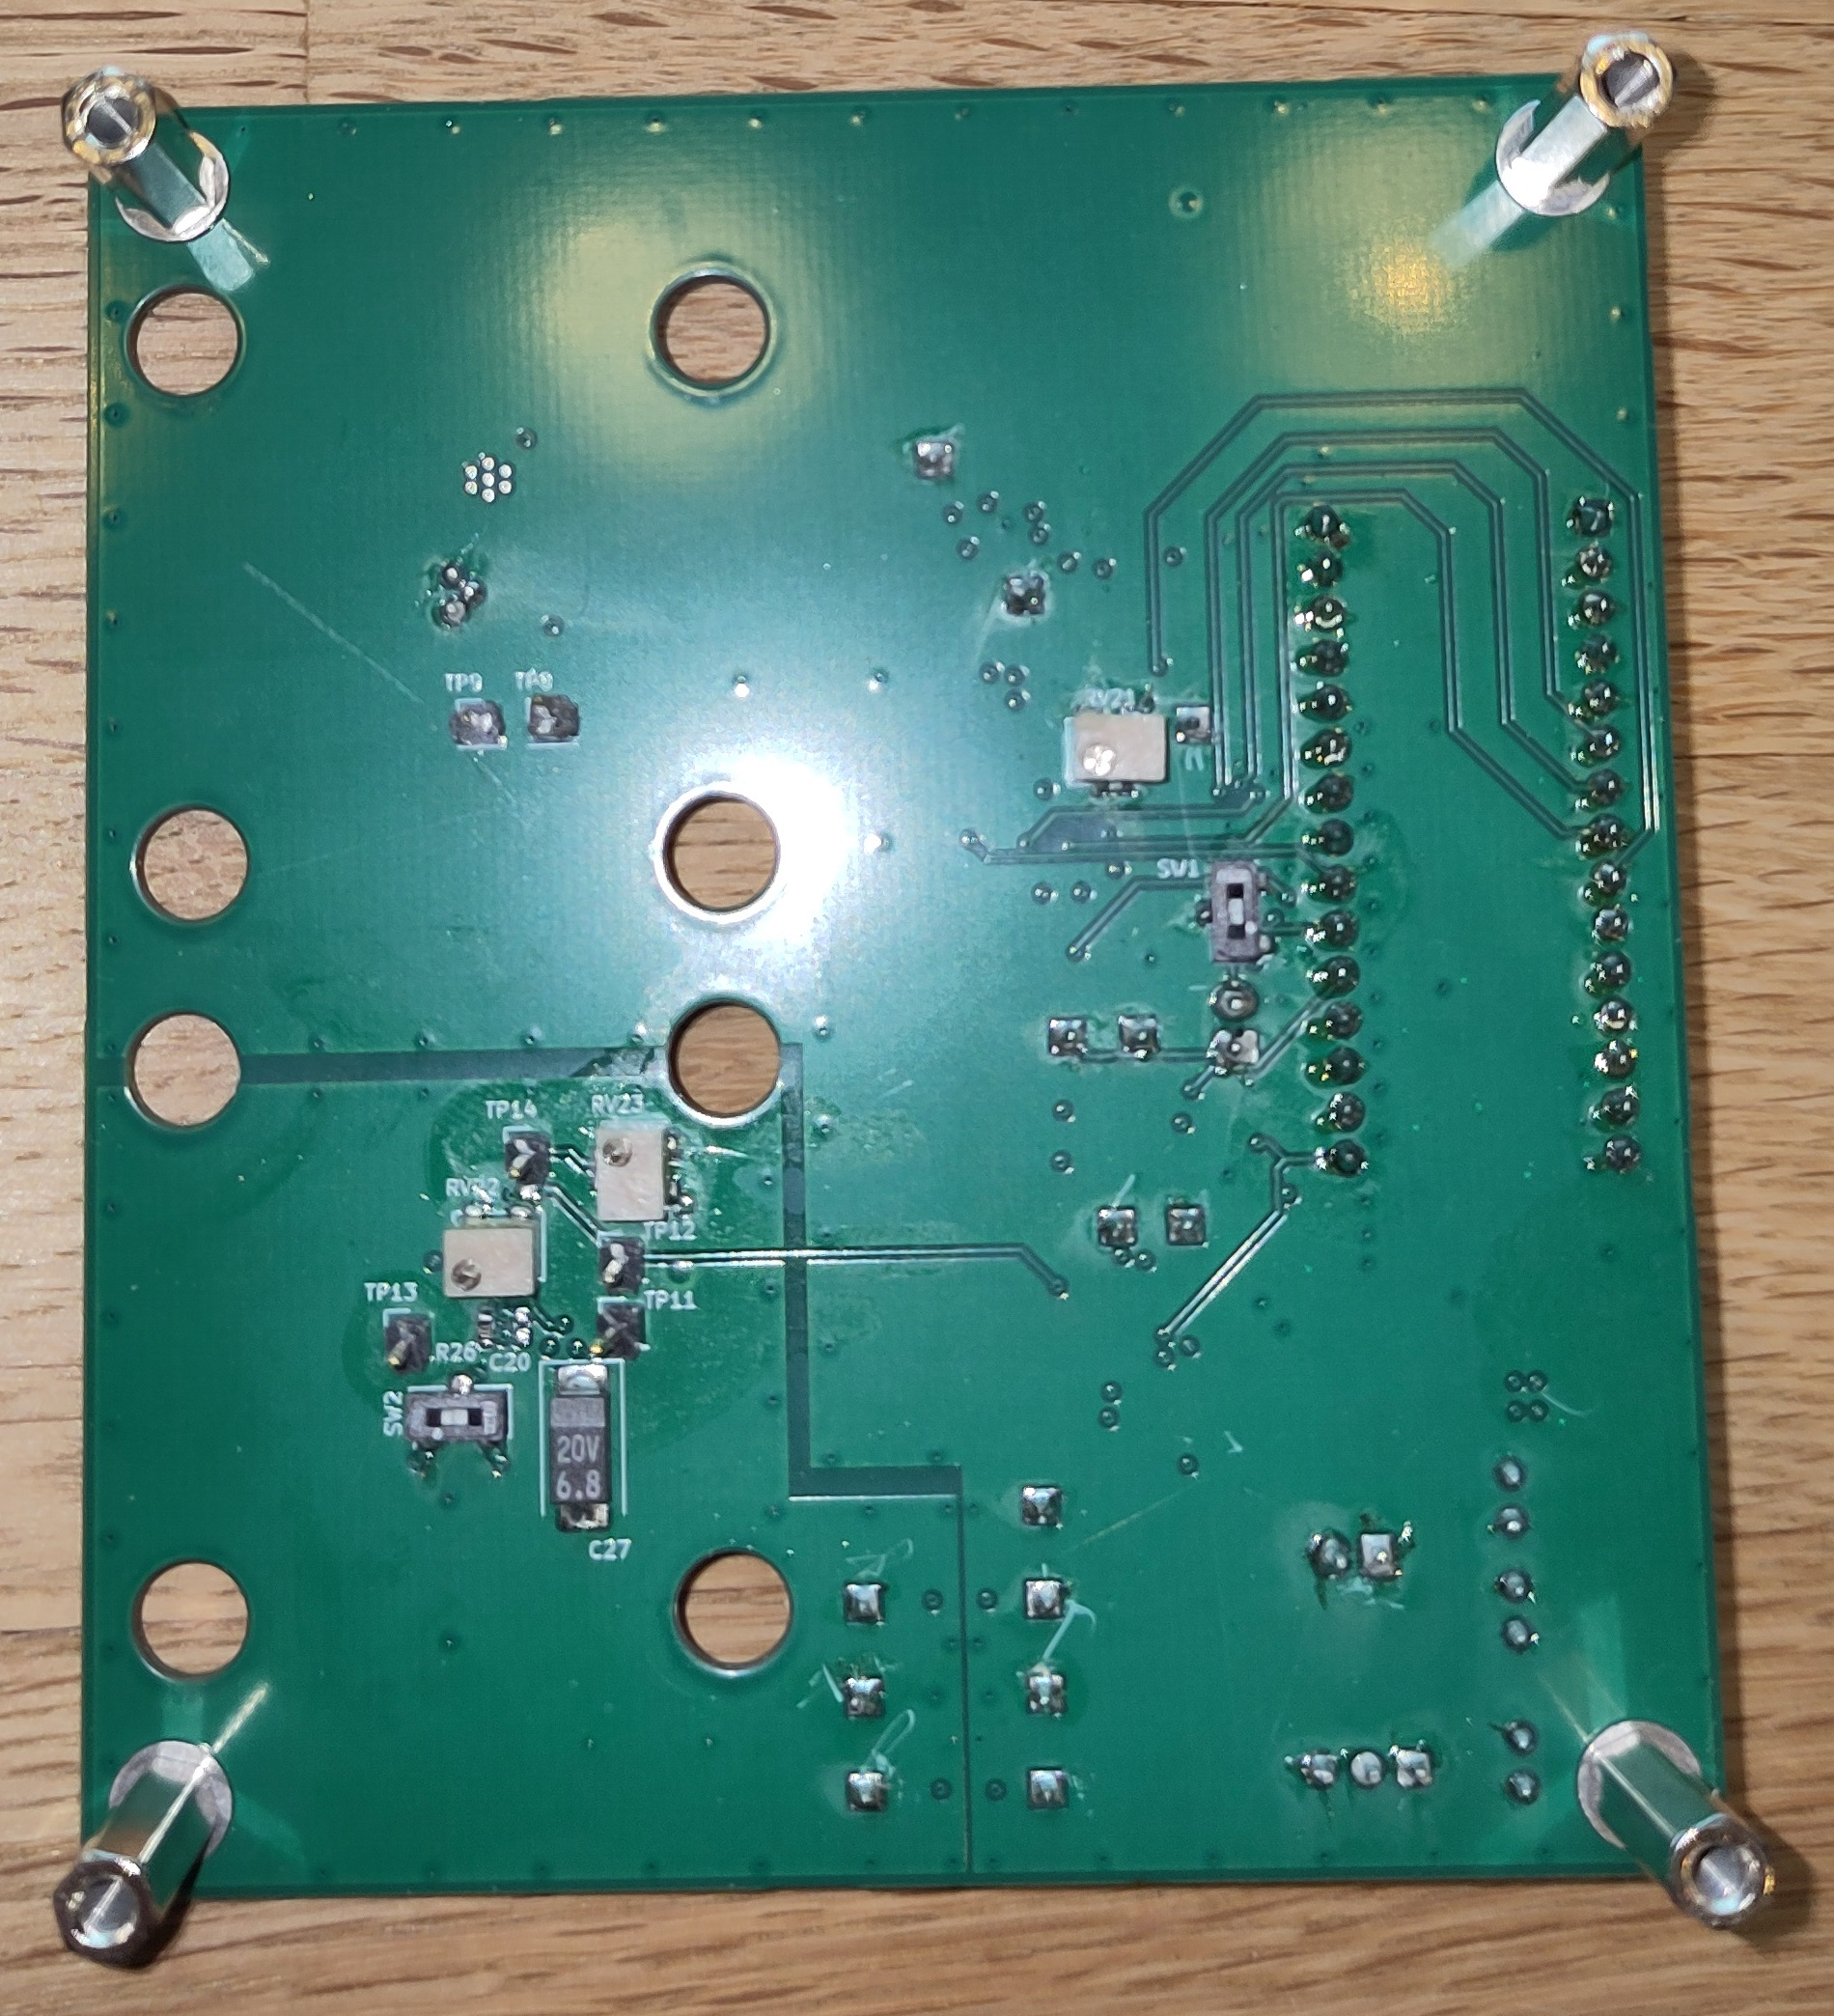
\includegraphics[width=0.6\textwidth]{graphics/photo_demonstrator_bottom.jpg}
    \caption{Demonstrator von unten}\label{fig:apdx_photo_demonstrator_bottom}
\end{figure}


%%%%%%%%%%%%%%%%%%%%%% CONTENT END %%%%%%%%%%%%%%%%%%%%%%

\pagebreak

\section*{Quellenverzeichnis}
\begin{flushleft}
\begingroup
\vspace{-25pt}
\renewcommand\refname{}
\renewcommand{\addcontentsline}[3]{} % Do not add bibliography to table of contents, as there is a separate subsection "Quellenverzeichnis"
\bibliography{references}
\endgroup
\end{flushleft}


\end{document}
